\documentclass[algorithmlist, figurelist,tablelist, nomlist, engineering, AutoFakeBold]{config/seuthesiY}
\usepackage{amsmath}
\usepackage{enumitem}
\usepackage{graphicx}
\usepackage{booktabs}
\usepackage{multirow}
\usepackage{listings}
\usepackage{xcolor}
\usepackage{enumitem}
\usepackage{array}
\usepackage{graphicx}
\usepackage{makecell}
\usepackage{subcaption}

\lstset{
    basicstyle=\ttfamily,        % 代码字体
    keywordstyle=\bfseries,      % 关键词加粗
    columns=fullflexible,        % 适应文本宽度
    frame=single,                % 加框
    breaklines=true,             % 自动换行
    postbreak=\hbox{$\hookrightarrow$}, % 换行符
    xleftmargin=10pt,            % 左边距
    float=false
}

%===============================================================================
% 采用的编译方式为  XELATEX -→  BIBER -→    XELATEX -→    XELATEX
% 为了加快字体的缓存效率 需要在命令行运行 fc-cache
% 对于学位论文需要标注【硕博】
%===============================================================================

% %biblatex宏包的参考文献数据源加载方式
\addbibresource[location=local]{config/seuthesiY.bib}

\begin{document}
%===============================================================================
\categorynumber{000} % 分类采用《中国图书资料分类法》
\UDC{000}            %《国际十进分类法UDC》的类号
\secretlevel{公开}    %学位论文密级分为"公开"、"内部"、"秘密"和"机密"四种
\studentid{222171}   %学号要完整,前面的零不能省略。
\title{积木世界VQA中的}{积木世界VQA中的}{空间推理问答技术研究与实现}{空间推理问答技术研究与实现}{Research and Implementation of Spatial Reasoning Questioning Answering Techniques }{in the Block World VQA}
\author{贾梁}{Jia Liang}
\advisor{张志政}{}{Zhang Zhizheng}{}
% \coadvisor{张志政}{副教授}{Zhang Zhizheng}{Associate Prof.} % 没有% 可以不填
\degreetype{工程硕士}{Master of Engineering} % 详细学位名称
\thesisform{应用研究} % 包括应用研究、调研报告、规划、产品开发、案例分析、项目管理、文学艺术作品、其它。非专业型硕士可忽略
\major{电子信息}
\submajor{计算机技术}
\defenddate{2025年5月30日}
\authorizedate{2025年6月20日}
\committeechair{翟玉庆}
\reviewer{倪庆剑}{张祥}
\department{东南大学计算机科学与工程学院}{School of Computer Science and Engineering}
\makebigcover
\makecover
\begin{abstract}{回答集编程,视觉问答,空间推理,神经符号方法}
积木世界是人工智能研究、教学、实验、评估的重要场景,能够模拟实际应用中物体间的空间关系。
积木世界VQA要求视觉语言模型(Visual Language Model, VLM)具备空间推理能力,但已有研究表明,当面对部分可见场景时,
其回答准确率显著下降。目前,通过结合神经网络和符号推理形成的神经符号模型,利用深度学习将视觉信息转化为逻辑符号,
再利用符号推理进行问题求解问题,比单纯依赖深度学习的视觉语言模型在空间推理任务中有更优异的表现。
由于回答集程序(Answer Set Program, ASP)是一种具备非单调推理和高效推理机的符号推理方法,
神经符号模型中采用ASP构建的神经符号VQA框架被寄予厚望。然而,现有框架设计中ASP规则的扩展仍依赖人工,
难以有效应对部分可见场景中基于空间推理的VQA任务。
    
针对上述问题,本文从构建积木世界部分可见场景中基于空间推理的VQA数据集、
设计规则自动补充的神经符号VQA方法、设计实现VQA课堂演示原型系统三个方面开展工作,具体如下:

\begin{enumerate}[itemsep=0pt]
\item 积木世界部分可见场景空间推理VQA数据集(Partial Observation VQA Dataset, POVQA\-D)构建。
CLEVR是空间推理的经典数据集,然而CLEVR中问题涉及的物体属性和物体间空间关系在图像中均完全可见,
通过引入部分可见性、遮挡机制与复杂空间关系模板,构建了覆盖部分场景可见问题的VQA数据集POVQAD。
该数据集将问题推理所需的平均步骤数从3提升到5,并新增了超 15\% 的空间封闭性与假设类问题,
且超过40\%的图像中包含不可见目标,比原数据集更能有效考察模型在部分可见场景中回答空间推理问题的能力。
\item 规则自动补充的神经符号VQA框架(Rule Complement Neuro-Symbolic Pipeline, RCNSP)设计。
RCNSP借鉴现有神经符号VQA框架的架构,新增规则蒸馏模块,
实现在ASP求解器进行推理前调用微调后的大语言模型自动对规则进行补充。
实验表明,在DeepSeek、LLaMA3、ChatGPT-4o三种大语言模型上,使用RCNSP比直接向VLM提问的准确率平均提升16.5\%,
比现有的神经符号VQA框架的准确率平均提升8.9\%,表明通过规则蒸馏能有效提升神经符号方法在部分可见场景中基于空间推理VQA中的效能。
\item 设计实现了一个积木世界VQA原型系统。在RCNSP框架和POVQAD数据集基础上,设计实现了一个
积木世界VQA原型系统。
该系统模拟了在自动规划课程的授课场景下,由教师向系统提出积木世界的空间推理问题,系统进行解答并展示推理的中间步骤和逻辑链条,
为教师向学生展示智能体如何理解外部环境信息并进行推理提供了便利。
初步测试表明该系统在CPU为Intel Core i9-12900K,内存128G,显卡为3张RTX 3090并联的硬件环境下,并发量为38,
90\%响应时间为6.9秒,能够满足自动规划课程教学场景下的用户需要。
\end{enumerate}

\end{abstract}

\begin{englishabstract}{Answer Set Programming, Visual Question Answering, Spatial Reasoning, Neuro-symbolic Method}
The block world is an important scenario for artificial intelligence research, education, experimentation, and evaluation, as it can simulate the spatial relationships between objects in real-world applications. Block world VQA requires Visual Language Models (VLMs) to possess spatial reasoning abilities; however, previous studies have shown that when faced with partially observable scenes, the answer accuracy significantly decreases. Currently, neuro-symbolic models that combine neural networks with symbolic reasoning—by using deep learning to transform visual information into logical symbols and then employing symbolic reasoning for problem solving—have demonstrated superior performance in spatial reasoning tasks compared to VLMs that rely solely on deep learning. Given that Answer Set Programming (ASP) is a symbolic reasoning method characterized by non-monotonic inference and efficient solvers, ASP-based neuro-symbolic VQA frameworks are highly anticipated. Nevertheless, the current framework designs still rely on manually expanded ASP rules, making it challenging to effectively address spatial reasoning VQA tasks in partially observable scenes.

To tackle the above issues, this work is conducted from three aspects: constructing a VQA dataset for spatial reasoning in partially observable block worlds, designing a neuro-symbolic VQA approach with automatic rule supplementation, and developing a prototype VQA classroom demonstration system. The specific contributions are as follows:
\begin{enumerate}[itemsep=0pt, parsep=0pt]
\item Construction of Partial Observation VQA Dataset (POVQAD).
CLEVR is a classical dataset for spatial reasoning; however, in CLEVR, 
all object attributes and spatial relationships are completely visible in the images. 
By introducing partial observability, occlusion mechanisms, and complex spatial relation templates, 
the VQA dataset POVQAD is constructed to cover partially observable scenarios. 
This dataset increases the average number of reasoning steps required per question from 3 to 5, 
adds more than 15\% of spatial closure and hypothetical reasoning questions, 
and includes over 40\% of images with invisible targets, 
thereby more effectively evaluating a model’s ability to answer spatial reasoning questions in partially observable scenes.
\item Design of the Rule Complement Neuro-Symbolic Pipeline (RCNSP).
The RCNSP framework builds on the architecture of existing neuro-symbolic VQA frameworks by introducing 
a rule distillation module. This module automatically supplements the rules using a fine-tuned large language 
model before the ASP solver performs reasoning. Experiments show that, across three large language models—DeepSeek, 
LLaMA3, and ChatGPT-4o—RCNSP achieves an average accuracy improvement 
of 16.5\% over directly querying VLMs and an 8.9\% increase over existing neuro-symbolic VQA frameworks. 
These results indicate that rule distillation can effectively enhance the performance of neuro-symbolic methods 
in spatial reasoning VQA tasks under partial observability.
\item Implementation of a VQA Classroom Demonstration Prototype System. 
Based on the RCNSP framework and the POVQAD dataset, a VQA prototype system is developed. 
This system supports the display of intermediate reasoning steps and logical chains when performing spatial reasoning
 tasks in response to user queries, thereby providing assistance for related research experiments and artificial 
 intelligence classroom instruction. Preliminary tests indicate that, under a hardware configuration of 
 an Intel Core i9-11900K CPU, 128 GB memory, and three RTX 3090 GPUs running in parallel, 
 with a concurrency level of 38 and a 90th percentile response time of 6.9 seconds, 
 the system meets the requirements of classroom teaching scenarios.
\end{enumerate}
\end{englishabstract}

\setnomname{术语与符号约定}
\tableofcontents
\listofothers
%===============================================================================


\mainmatter

\chapter{绪论}
\section{研究背景}
随着计算机视觉(Computer Vision)
和自然语言处理(Natural Language Processing)技术的迅猛发展,
跨模态智能理解成为人工智能研究的重要方向之一。
其中,视觉问答(Visual Question Answering, VQA)\cite{goyal2017making}任务因其广泛的应用前景和挑战性,
受到了学术界和工业界的广泛关注。例如,给定一幅包含动物的图片,
系统需要能够回答“这只动物是什么颜色?”或“图片中有几只猫?”等问题。
这一任务的核心在于多模态信息的深度融合,即如何在视觉特征和语言信息之间建立有效的联系。
积木世界\cite{hogg1983block}是人工智能研究、教学、实验、评估的重要场景,能够模拟实际应用中物体间的空间关系。
研究积木世界VQA任务,能够有效考察智能体在空间推理方面的能力。
积木世界可通过对不同复杂度的场景的模拟,能够作为范例方便用于大语言模型、自动规划、自然语言处理、模式识别等
不同方向的研究和课程的教学中\cite{chiyahgarcia2024repairsblockworldnew}\cite{silver2023generalizedplanningpddldomains}。
研究积木世界VQA任务,通过不同的积木摆放、堆叠、遮挡等空间布局的积木世界数据,
能够有效地用于研究和考察智能体在空间推理方面的能力\cite{johnson2017clevr}。

多年以来,有多种方法被提出用于解决VQA任务,其中
视觉语言模型(Visual Language Model, VLM)因其强大的多模态理解能力而备受关注。
VLM是一种多模态模型,能够同时处理图像和文本信息,并生成与图像内容相关的自然语言响应。
如图\ref{fig:vlm-example}所示为VLM的一个简单流程示例。
VLM通过将视觉编码器与大语言模型结合,赋予模型“看”与“理解”的能力。与传统的计算机视觉模型不同,VLM 不受固定
类别集或特定任务 (如分类或检测) 约束。在大量文本和图像/视频字幕对的语料上进行重新训练,
VLM 可以用自然语言进行指导,并用于处理许多典型的视觉任务以及新的生成式 AI 任务,
例如摘要和视觉问答。如图\ref{fig:vlm-architecture}所示为VLM的通用架构,包括视觉编码器、投影器和大语言模型(Large Language Model, LLM)三个部分。
视觉编码器(如CLIP模型)具有图像与文本的关联能力,负责提取图像特征。投影器由一组网络层构成,负责将视觉特征转换为LLM可理解的标记(Token)。
LLM负责生成文本输出,支持对话、推理等任务,目前任何现有的LLM(如ChatGPT、LLaMA、DeepSeek等)都可以用来构建VLM。
\begin{figure}
    \centering
    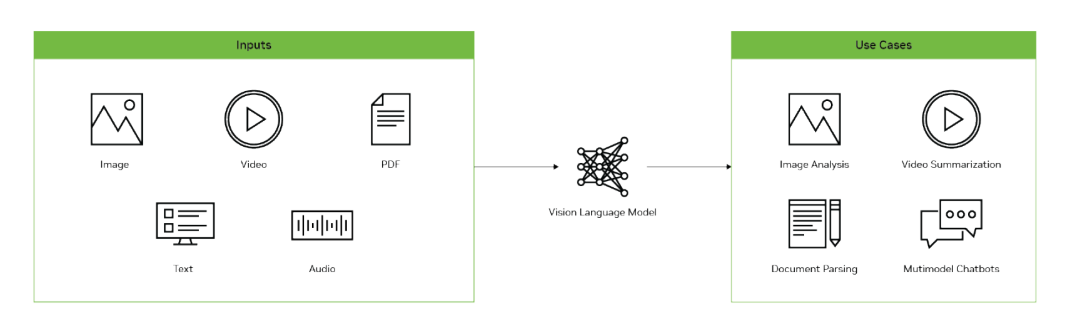
\includegraphics[width=\textwidth]{figures/VLM-example.png}
    \caption{视觉语言模型用例}
    \label{fig:vlm-example}
\end{figure}

\begin{figure}[htb]
    \centering
    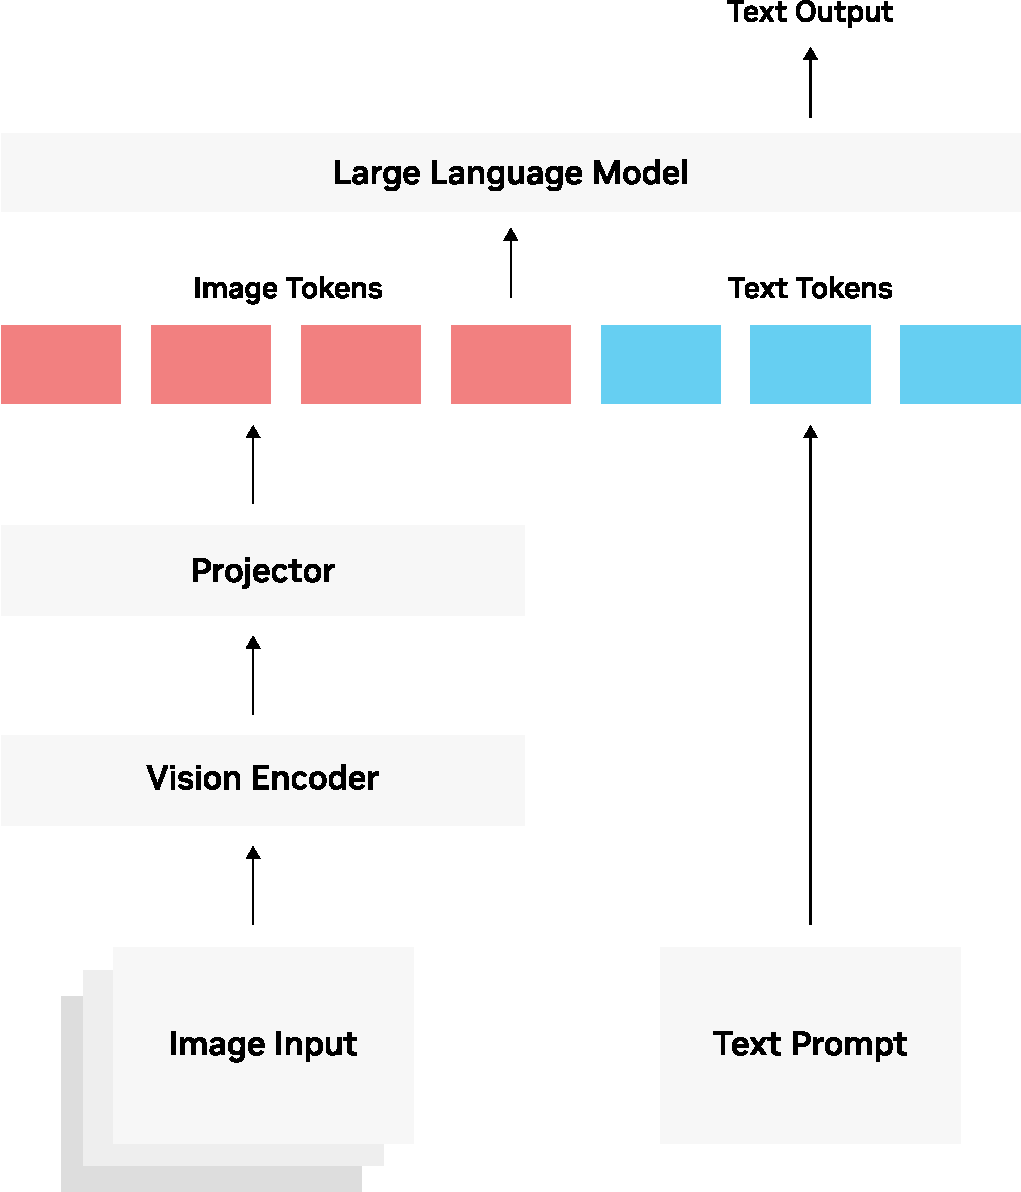
\includegraphics[scale=0.6]{figures/vlm-architecture-diagram-crop.pdf}
    \caption{视觉语言模型的通用三部分架构}
    \label{fig:vlm-architecture}
\end{figure}

尽管VLM在图像分类\cite{pratt2023does}、字幕生成\cite{alaluf2024myvlm}、
目标检测\cite{kuo2022f}、视频理解\cite{huang2024lita}和文档解析\cite{lv2023kosmos}
等各种任务中取得了良好效果,但VLM仍难以有效应对部分可见场景中基于空间推理的VQA任务。
部分可见指的是在图像中,某些物体或其特征由于遮挡、模糊、视野受限、噪声或其他原因而不可见的情况,
导致模型无法从图像中获得解决问题所需的全部信息。
现有的VLM在部分可见场景中解决VQA任务时,可能会出现幻觉\cite{vardi2025clipupclipbasedunanswerableproblem}
、空间关系推理能力下降\cite{chen2024spatialvlmendowingvisionlanguagemodels}\cite{anis2025limitationsvisionlanguagemodelsunderstanding}
,并且在对象识别和计数任务中表现不佳\cite{campbell2024understandinglimitsvisionlanguage},不能真正理解图像信息\cite{rahmanzadehgervi2025visionlanguagemodelsblind}等问题。
这类部分可见场景在现实世界中广泛存在,例如在机器人抓取、自动驾驶、安防监控等实际应用中,
系统往往需要在信息不完全的条件下对场景作出准确理解和决策。

因此,研究能够在部分可见场景中进行准确空间推理的VQA方法,不仅具有理论挑战性,也具有重要的工程价值。
一方面,它有助于提升人工智能系统在复杂环境中的稳健性和泛化能力;
另一方面,也为智能机器人\cite{gao2024physically}\cite{nasiriany2024pivot}、
AR/VR交互系统\cite{konenkov2024vr}等场景中的感知与决策提供了新的技术路径。

为了解决多模态模型在空间推理方面的问题,研究者们提出了一些新的方法。近年来,
神经符号方法(Neuro-Symbolic Methods)得到了广泛关注。在多模态空间推理场景中,
神经符号方法使用深度学习技术进行感知,为输入的图像和问题分别生成符号表示,再使用符号系统进行推理求解,
可以有效提升多模态模型在空间推理方面的能力。

在神经符号方法中,神经网络的选择十分多样,通常包括卷积神经网络(Convolution Neural Network, CNN)、
循环神经网络(Recurrent Neural Network, RNN)及其变体、图神经网络(Graph Neural Network, GNN)和
Transformer架构及LLM。相比其它神经网络,LLM用于神经符号系统,具有以下突出优势:
\begin{enumerate}[itemsep=0pt,parsep=0pt]
    \item 丰富的预训练知识库。LLM在大规模语料上进行预训练,具备广泛的世界知识和语言理解能力,这使得它们在处理涉及常识推理和多领域知识整合时,比专门针对单一任务训练的网络更具优势。
    \item 自然语言理解与生成能力。LLM能够将符号系统产生的抽象逻辑或规则,用自然语言进行解释和反馈,从而降低了人机交互的门槛,并使得系统的推理过程更易于理解和验证。
    \item 零样本/少样本学习能力。由于在大规模数据上学习到了通用的语言模式,LLM在面对新领域或数据较少的任务时,往往能够直接发挥作用,从而提高神经符号系统的泛化能力。
    \item 灵活的上下文建模。LLM能够捕捉长距离依赖和上下文信息,这对于将符号系统中离散的知识点进行有机整合,以及在复杂场景中实现动态推理具有重要意义。
\end{enumerate}
结合以上各项理由,将LLM作为神经符号系统中的神经模块,能够与符号系统形成互补,既利用符号逻辑的严谨性,又发挥神经网络在语义理解和自然语言生成方面的优势,从而构建更强大、更灵活的智能系统。

在神经符号方法中,符号系统的选择同样多种多样,例如知识图谱嵌入(Knowledge Graph Embeddings, KGE)、逻辑神经网络(Logical
 Neural Networks, LNN)都为信息表示和推理提供了新思路。其中,回答集编程(Answer Set Programming,ASP)也被
越来越多地采用作为符号系统。ASP是一种声明式编程范式,可用于解决复杂的人工智能问题,其起源于对逻辑编程、非单调推理和知识表示的研究。
相比其它符号系统,ASP被更多用于神经符号方法中,主要是由于以下几点优势:(1)明确的逻辑语义与可解释性。ASP基于严格定义的逻辑规则,其推理过程透明、易于解释。这一特性在需要精确推理和结果可验证的任务中尤为重要\cite{gelfond1988stable};
(2)强大的非单调推理能力。ASP自然支持非单调逻辑推理,能够处理默认情况和异常情形,这使其在面对现实世界中不完全或动态变化的信息时表现出色\cite{gelfond1988stable};
(3)成熟的求解器与工具支持。像Clingo这样的ASP求解器已经经过长期验证,具有高效、稳定的特点,能够处理大规模问题,这为实际应用提供了有力保障\cite{gebser2012answer};
(4)便于与神经网络等模块整合。ASP的声明式表达方式使其易于与神经网络输出的信息对接,形成互补优势,从而提升整体系统的推理能力\cite{garcez2002neural}。
ASP的这些特性使得它作为符号系统的杰出代表,被广泛应用于神经符号方法中。

尽管神经网络采用了预训练的LLM,而符号系统部分选用了ASP,但将二者有效结合在一起仍然是一项复杂的任务。
为此,近年来出现了一些神经符号框架,试图通过模块化设计和统一接口来简化LLM与ASP的集成开发流程\cite{wang2024dspybasedneuralsymbolicpipelineenhance}。
尽管现有的框架为LLM结合ASP的开发过程提供了诸多便利,降低了使用门槛,然而其在ASP规则的自动拓展方面存在不足,
需要依赖人工干预进行规则扩充,在这一方面仍存在改进空间。

为了测试模型解决空间推理问题的能力,涌现了诸如CLEVR、GQA、COCO等数据集。
这些数据集由问题答案对(Question and Answer Pair,以下简称QA对)组成,
并且包含问题对应的场景图像。CLEVR是一种积木世界的数据集,因其高度结构化的场景构造、精确标注的物体属性及复杂的空间关系,
而被广泛用于人工智能的研究和课堂教学等重要场景。
然而,CLEVR数据集图像均基于完整场景生成,所有回答问题的信息都直接可见,缺乏现实环境中常见的部分可见性,
难以有效考察VLM在部分可见场景中的推理能力\cite{sam-abraham-etal-2024-clevr}。
因此,要考察模型在部分可见积木世界中对空间推理问题的解答能力,需要对CLEVR进行改进,以使其具备部分可见性。

自动规划作为人工智能领域的一个重要分支,其核心目标是让计算机能够像人类一样,自主地制定实现特定目标的行动计划。
对能够完成积木世界中寻找、挪动物体等任务的智能体而言,空间推理显然是其能够完成任务指令的前置要求。
目前,市面上业已出现不少人工智能课程教学的演示系统,然而很少有演示教学系统
关注自动规划课程中的积木世界空间推理,不能展示智能体运用哪些知识以完成空间推理,进而达到最终目标。
为此,设计并实现一个自动规划课堂教学演示原型系统,展示智能体如何在部分可见的积木世界场景下完成空间推理,
对启发学生理解人工智能思考过程,进一步提升自动规划课程教学的可视化水平,具有十分重要的意义。

综上所述,积木世界作为空间推理研究的重要场景,虽在可视化、可控性和评估便利性方面具备显著优势,
但现有视觉语言模型在面对部分可见或遮挡场景时,其空间推理能力仍显不足。
神经符号方法通过引入形式化的逻辑推理机制,有效弥补了深度学习在可解释性和系统性推理方面的短板,
尤其是在复杂空间关系建模中展现出潜力。然而,当前神经符号VQA框架中ASP规则的拓展仍主要依赖于人工,
难以灵活适应动态环境和多样化任务需求。为进一步提升神经符号模型在部分可见场景中的空间推理性能,
亟需构建具挑战性的高质量数据集,并探索规则自动补充机制与大语言模型的协同方式,
从而推动视觉问答系统在积木世界场景中的智能推理能力发展,为自动规划课堂中教师向学生展示智能体如何理解外部环境信息并进行推理提供了便利。
\section{相关研究现状}
基于前述背景,本文的研究目标明确为:提升神经符号方法用于部分可见的积木世界的空间推理问答的准确率。
为达成该研究目标,所需了解的
研究领域包括VQA技术、VQA数据集、ASP程序生成、空间推理、神经符号方法在空间推理中的应用等。为此,本节将对这些领域的相关研究进行综述。
\subsection{VQA技术的研究现状}
VQA是由Antol等人\cite{Antol2015VQA}提出的,是人工智能领域中一个富有挑战性的交叉研究方向,
涉及计算机视觉(CV)、自然语言处理(NLP)和机器学习(ML)等多个学科。
其核心任务是让机器能够根据给定的图像内容和相关的自然语言问题,生成准确的自然语言答案。
VQA不仅要求模型理解图像中的视觉信息(如物体、属性、关系)和问题的语义意图,还需要进行复杂的推理,
融合这两种模态的信息来找到或生成答案。近年来,随着深度学习技术的发展,VQA领域取得了显著进展,但也面临着诸多挑战。

早期的VQA模型通常采用相对简单的框架,例如使用卷积神经网络(CNN)提取图像特征,使用循环神经网络(RNN)
或长短期记忆网络(LSTM)编码问题,然后通过简单的融合策略(如元素积、拼接)结合两种模态的特征,最后输入到一个分类器中预测答案。

然而,这类方法难以有效关联问题中的关键信息和图像中的特定区域。为了解决这个问题,注意力机制
被广泛引入VQA模型中。其核心思想是让模型根据问题的指导,动态地聚焦于图像中最相关的区域。其中, Anderson等人提出的自下而上的注意力机制\cite{anderson2018bottom}
成为后续许多模型的基础。该方法首先使用Faster R-CNN等目标检测器提取图像中的显著区域,
然后根据问题生成一个查询向量,计算该查询与各个区域特征的相似度(注意力权重),最后对区域特征进行加权求和,
得到与问题高度相关的视觉特征。这种方法显著提升了模型性能,因为它能更精确地定位与问题相关的视觉证据。
后续研究进一步发展了注意力机制,如分层注意力\cite{lu2016hierarchical}和共同注意力,后者允许模型同时学习图像区域和问题词语之间的相互关联,从而实现更深层次的跨模态信息交互。

随着Transformer架构在NLP领域的巨大成功,研究者们也开始将其应用于VQA任务,以更好地捕捉长距离依赖和模态间的复杂交互。
这些模型通常利用Transformer的自注意力和交叉注意力机制。ViLBERT\cite{lu2019vilbert}和 LXMERT\cite{tan2019lxmert}是早期的代表性模型。
它们采用双流架构,分别处理视觉和文本输入,并通过跨模态Transformer层进行信息交互和融合。VL-BERT\cite{su2019vl}和 Oscar\cite{li2020oscar}则采用了单流架构,
将图像区域特征和文本词嵌入拼接在一起,输入到一个统一的Transformer编码器中进行联合建模。Oscar还引入了目标标签作为“锚点”,
连接图像区域和对应的文本描述,增强了跨模态对齐。

这些基于Transformer的视觉语言预训练(Vision-Language Pre-training, VLP)模型通常在大规模的图像-文本对数据上进行预训练,
学习通用的跨模态表示,然后在特定的VQA数据集上进行微调,取得了显著的性能提升。

近年来,LLM如GPT-3、PaLM等在自然语言处理任务上展现了惊人的能力。
研究者们迅速探索了将LLM应用于VQA领域,催生了大型多模态模型(Large Multimodal Model, LMM) 或 
VLM的研究热潮。这类模型通常利用预训练好的强大LLM作为基础,通过设计特定的接口或适配器将视觉信息“注入”到LLM中,使其能够理解图像内容并回答相关问题。
OpenAI发布的GPT-4V\cite{openai2023gpt4v}展示了前所未有的多模态理解和推理能力,
能够处理复杂的视觉问答、图像描述、图表解读等任务。虽然其具体架构和训练细节未完全公开,但它代表了当前LMM能力的顶尖水平。

基于LLM的VQA模型通常具有更强的零样本/少样本泛化能力、更自然的语言交互能力、更好的常识推理能力,
并且能够处理更开放式、更复杂的查询。它们将VQA从一个多模态分类/生成任务,转变为一个基于视觉信息的条件语言生成任务。

尽管VQA领域取得了巨大进步,但仍面临一些挑战。
第一是深度推理与组合性。模型在处理需要多步逻辑推理、精确计数或复杂空间关系的问题时仍然困难。
第二是鲁棒性与偏见。模型容易受到对抗性样本攻击,并且可能学习到数据集中的统计偏见,而非真正的视觉理解。
第三是可解释性。理解模型为何给出特定答案仍然是一个挑战,尤其对于复杂的黑箱模型。
第四是知识依赖。如何更有效地融合和利用外部世界知识或领域知识来回答专业性或常识性问题。
第五是效率与部署。大型多模态模型通常计算量巨大,如何在资源受限的设备上高效部署是一个实际问题。
\subsection{VQA数据集的研究现状}
VQA作为跨模态推理的重要任务,近年来在VQA数据集建设方面取得了显著进展。
早期的VQA v1.0与v2.0数据集主要基于真实图像,问题类型以事实性提问为主,虽然具备一定规模,
但在逻辑推理深度和场景可控性方面存在明显局限。因此,研究者逐步转向使用合成图像生成更具可控性和推理复杂度的数据集,
以更有效地评估模型的逻辑与空间推理能力。

CLEVR\cite{johnson2017clevr}是该方向中的代表性数据集,被广泛用于评估模型在属性识别、比较、空间关系理解等方面的能力。
该数据集通过精心设计的合成场景和程序化生成的问题模板,有效规避了偏差问题,同时提供了清晰的程序标注,
使其成为神经符号推理方法的标准测试平台。尤其在空间关系理解方面,CLEVR提供了诸如“左边的球是什么颜色?”、
“与红色立方体相邻的物体有多少个?”等类型的问题,涵盖了多种空间方位与拓扑关系,为开发具备空间推理能力的模型提供了重要实验基础。

本文课题以积木世界为背景,而CLEVR数据集在任务设定和场景设计上,与积木世界有高度相似性:
同样使用规则几何体组合构建三维场景,并注重问题的组合推理特性。
因此,CLEVR不仅为本文提供了可借鉴的数据构造方法,也验证了基于合成场景推动空间推理研究的有效性。

然而,CLEVR在设计上假设场景信息完全可见,即观察者可以从固定角度完整获取所有物体的属性与相对关系。
这种全可见性的假设简化了推理难度,却与现实环境中部分可见场景存在显著差异。部分可见性常见于机器人导航、现实场景感知等任务中,
在这种情况下,模型不仅要理解空间关系,还需在不完全信息下进行补全与推断。
此外,CLEVR并不要求模型在回答问题时主动使用图像场景以外的背景知识或逻辑约束,模型主要使用对图像内容的直接理解
和内部逻辑进行推理,并不能充分考察模型利用现有常识进行推理的能力。
由此看来,CLEVR虽然在空间推理研究中奠定了坚实基础,
但仍难以满足部分可见积木世界的问答任务的需求。

因此,以CLEVR数据集为基础,将部分可见性引入CLEVR数据集,对研究部分可见的积木世界中的空间推理问答任务具有重要意义。
\subsection{生成ASP程序的研究现状}
本研究旨在提升神经符号方法在部分可见的积木世界空间推理问答任务中的准确性,其中ASP程序的自动生成能力是关键组成部分之一。
积木世界中的空间问答不仅要求模型理解图像中的空间结构并生成对应的逻辑程序,还需将自然语言问题转换为逻辑形式进行推理。
在这一过程中,如何高效、准确地生成ASP代码,直接影响到神经符号系统的整体推理效果与任务完成度。
以下将对当前自动生成ASP程序的研究现状进行综述。

近年来,代码自动生成技术在学术界和工业界均得到了广泛关注与深入研究。
已有研究表明,自动合成程序具有显著的效率与准确性优势 \cite{ernst2022ai}\cite{peng2023impact}\cite{dakhel2023github},
并已广泛应用于几乎所有主流的命令式编程语言中 \cite{chen2021evaluating}。
其中,大型语言模型(LLMs)作为核心技术手段,在代码生成任务中表现出了极强的能力,并在多个基准测试中得到了系统性的评估 \cite{xu2022systematic}\cite{wang2023codet5+}。同时,也有研究指出,通过针对特定任务微调模型可以进一步提升其在命令式语言代码生成中的表现 \cite{ma2024llamoco}。

在声明式编程领域,尤其是针对答案集程序设计(Answer Set Programming, ASP)的自动生成,
同样引起了研究者的广泛关注。相关研究主要致力于构建工具,自动将自然语言规范转换为ASP程序,
以缩短自然语言表达与逻辑程序之间的语义距离 \cite{erdem2009transforming}\cite{fang2017approach}\cite{schwitter2018specifying}\cite{caruso2024cnl2asp}。早期的研究主要集中于将简化英语表述的逻辑谜题自动转化为ASP程序,通过λ演算与概率组合范畴语法等方法进行语义解析 \cite{baral2012solving}。

随后,研究者提出了“受控自然语言(Controlled Natural Languages, CNLs)”的概念,
用于在保留自然语言可读性的同时,满足逻辑编程所需的形式化表达要求 \cite{kuhn2014survey}。
Erdem等人提出了BIOQUERYCNL语言并给出了其向ASP查询语句转译的算法 \cite{erdem2009transforming};
Fang等人基于LANA注解机制,设计了一套适用于SeaLion IDE的CNL构造方案 \cite{fang2017approach};
2018年,Schwitter开发了PENGASP语言,用于ASP程序的语言化与可视化表达 \cite{schwitter2018specifying}。
近年来,Dodaro等人推出的CNL2ASP工具实现了从CNL到ASP的自动转换,并已公开发布,成为该领域的一项重要成果 \cite{caruso2024cnl2asp}。
尽管CNL显著降低了ASP的使用门槛,为非专业用户提供了更为自然的表达方式,
但其语法与词汇依然受到约束,仍然要求用户具备一定的形式化语言构造能力,限制了其普适性与灵活性。

随着大型语言模型的发展,研究者开始尝试将其与ASP系统相结合,从而在自然语言理解与逻辑推理之间建立更直接的连接。
Nye等人提出的“双系统模型” \cite{nye2021improving},利用GPT-3生成自然语言语义解析器,并与ASP推理模块进行集成,
显著提升了系统的推理能力与泛化性能。
Yang等人进一步验证了GPT-3作为少样本语义解析器的可行性,
能够在无需专门微调的情况下将自然语言问题直接转化为ASP格式的逻辑表达 \cite{yang2023coupling}。
此外,Ishay等人结合提示工程技术,基于Mitra等人的逻辑谜题数据集,构建了ASP自动求解系统 \cite{mitra2016addressing};
Rajasekharan等人则在STAR框架中系统性地实现了LLMs与ASP的结合,用于多种自然语言理解任务 \cite{rajasekharan2023reliable}。

尽管已有研究已初步展示了LLMs在ASP生成方面的潜力,但系统性面向声明式语言(特别是ASP)代码生成的研究仍较为匮乏。
2024年,Borroto等人提出并实现了NL2ASP工具 \cite{borroto2024automaticcompositionaspprograms},该工具基于两阶段架构:
首先通过神经机器翻译模型(如T5-small、Bart-base)将自然语言转换为受控自然语言形式;随后借助CNL2ASP工具生成对应的ASP程序。
该方法在图结构类问题中展现出较好效果,是将LLMs用于ASP程序自动生成的重要探索之一。

然而,NL2ASP方法仍存在诸多限制:其一,其适用范围主要集中在图相关问题,通用性较弱;
其二,采用中间表示形式(CNL)增加了系统复杂性,可能引入额外的误差与信息损失;
其三,虽然作者指出了LLMs在ASP代码生成中的低表现,但尚缺乏系统性、全面的实证分析。

综上所述,当前针对ASP程序的自动生成研究已取得初步进展,
从早期的受控自然语言设计到近年来结合大语言模型(LLMs)进行语义解析与代码合成,相关技术不断演进。
以上这些研究为进一步提升ASP程序自动生成的准确率,拓展ASP的应用范围并提升神经符号方法在积木世界空间推理问答任务中的表现提供了
研究空间与创新方向。
\subsection{空间推理的研究与现状}
空间推理涉及对物体位置、方向、距离以及相互关系的理解和处理,是计算机视觉、自然语言处理以及机器人导航等领域的核心能力。
尽管人类在空间推理上有天然优势,但当前的模型(尤其是大语言模型和视觉语言模型)在这方面仍面临不少挑战。
这一问题催生了大量针对空间推理能力提升的研究工作。

基于规则的符号推理最早被用于解决空间推理问题,其核心思想是使用几何约束(如欧氏距离、拓扑关系RCC8)和逻辑推理(如谓词逻辑)建模空间关系。
Allen等人提出了相关方法。然而,这种方法过于依赖人工规则,难以处理复杂场景和非结构化数据,实际应用价值有限。后来,有一部分研究者将概率图模型引入到空间推理问题中。
Kuipers等人提出空间语义层次模型,结合贝叶斯网络或马尔可夫随机场(MRF)建模空间关系的不确定性。

进入2010年代,深度学习方法开始快速发展,一些研究者将深度学习方法引入空间推理领域。Antol等人\cite{Antol2015VQA}提出使用CNN+LSTM直接预测
空间问题的答案,Xu等人\cite{xu2017scene}提出使用场景图生成的方法检测物体及其空间关系。这些端到端神经网络的方法,都是黑箱模型,缺乏可解释性,且易受数据偏差影响。
后来有研究者尝试使用图神经网络解决空间推理问题,将场景建模为图结构,通过消息传递捕捉空间关系。

2023年,以OpenAI的ChatGPT广受世界关注为标志,LLM得以迅速发展。以LLM为重要组成部分的VLM得以快速发展,应用于空间推理问题的解决中。
研究者致力于增强VLM的空间推理能力,取得了一系列重要成果。
例如,Google DeepMind开发的SpatialVLM\cite{chen2024spatialvlmendowingvisionlanguagemodels}项目通过生成并训练一个大规模3D空间视觉问答(VQA)数据集,
显著提升了VLM在空间推理任务中的表现。该研究利用互联网规模的真实世界图像,自动标注了约1000万张图像和20亿个VQA示例
(其中50\%为定性,50\%为定量),在二元谓词预测任务中达到了75.2\%的准确率,远超GPT-4V(68.0\%)和LLaVA-1.5(71.3\%)。
此外,SpatialVLM在定量问题中输出数字的比率达到99.0\%,其中37.2\%的答案落在[50, 200]\%的范围内,展示了其在链式思维空间推理和机器人应用中的潜力,
如为机器人任务提供密集奖励注释。

另一项研究SpatialRGPT\cite{cheng2024spatialrgptgroundedspatialreasoning}通过引入数据整理管道和灵活的“插件”模块,
整合深度信息到视觉编码器中,增强了VLM在3D空间认知中的表现。该研究提出了SpatialRGBT-Bench基准,包含室内、外和模拟环境的3D注释,
用于评估VLM在复杂环境下的空间推理能力。这些进展表明,通过大规模数据训练和多模态信息整合,VLM的空间推理能力得到了显著提升。

尽管VLM在空间推理任务中取得了一定的进展,但VLM仍在部分可见场景中存在一些局限性,主要体现在以下几个方面:
\begin{enumerate}[itemsep=0pt,parsep=0pt]
\item 幻觉现象。当视觉信息不完整时,VLM 往往会生成不正确或虚构的答案,
即“幻觉”出图像中不存在或无法从可用视觉线索中可靠推断出的细节。这种趋势在问题涉及完全缺失的对象时可能尤为明显,
尽管模型对答案充满信心,实际上却给出了错误答案\cite{vardi2025clipupclipbasedunanswerableproblem}。
\item 空间关系推理能力下降。理解对象之间如“后面”或“旁边”的空间关系通常依赖于完整或足够的视觉线索。
当场景中的某些部分由于遮挡或视野受限而缺失时,VLM对空间关系的准确辨识能力会受到严重影响,甚至出现逃避或胡乱回答的现象\cite{chen2024spatialvlmendowingvisionlanguagemodels}。
\item 部分基本任务出现失败。有研究指出,在部分可见场景下VLM在一些基本的多对象推理任务(如计数和定位)上的表现不佳\cite{campbell2024understandinglimitsvisionlanguage}。
\end{enumerate}

这些局限性表明,当前基于LLM的VLM仍难以有效应对基于空间推理的VQA任务,特别是在出现遮挡、视野受限、噪声等情形的部分可见场景中。
\subsection{神经符号方法应用于空间推理中的研究现状}
为克服上述局限,研究者开始探索神经符号方法,将神经网络的模式识别能力与符号推理的逻辑表达能力相结合。
神经符号方法通过显式表示空间关系和逻辑规则,能够更好地处理复杂推理任务,尤其是在多跳推理和泛化能力方面。

最早将神经符号方法用于空间推理的工作是由Andreas等人\cite{andreas2016neural}提出的Neural Module Network(NMN),其核心思想是:NMN通过模块化分解,将复杂推理拆解为可复用子模块的动态组合,
使模型能根据问题语义动态调整计算路径。最终在CLEVR数据集上实现了超过90\%的准确率,显著优于传统的CNN-LSTM模型。这一开创性的工作,为
后续神经符号推理的研究奠定了基础。

Yi等人\cite{yi2019neuralsymbolicvqadisentanglingreasoning}在Andreas等人的工作基础上,提出了Neural-Symbolic VQA(NS-VQA)模型,
通过设计神经符号解耦框架,将视觉感知、语言理解和符号推理解耦,以减少跨模态耦合带来的偏差放大效应,并通过符号程序将问题转化为可执行的推理步骤,避免端到端模型对语言表面模式的依赖。
最终实验结果表明,NS-VQA在CLEVR数据集上达到了94.5\%的准确率,验证了神经符号方法在空间推理中的有效性。此外,NS-VQA通过分离语言理解和视觉推理,模型对语言分布偏移的敏感性降低,性能提升约15\%。
该成果是神经符号融合的样板性工作,首次在VQA中系统整合符号推理与深度学习,为后续神经符号AI研究提供方法论基础,也为对抗语言先验提供了一种解决方案,
推动VQA从“模式匹配”向“真实理解”演进。

后续,Yang等人\cite{yang2020neurasp}提出了NeurASP这类方法在 NS‐VQA 的基础上引入了神经原子(neural atom)和选择规则,
用以更灵活地处理对象检测的不确定性,缓解了对强监督程序注释的依赖,并在一定程度上改善了符号执行模块的透明性。Thomas等人\cite{eiter2022neuro}对NeurASP中进行改进,在ASP编码和不确定性管理上采用了基于统计门槛的筛选策略,
致力于提高系统的效率和鲁棒性,同时更明显地解耦视觉感知与符号推理,使得推理过程更加透明和可解释。

随着LLM在2023年的迅速发展,越来越多的研究者将LLM引入到神经符号方法中,取代传统的CNN、RNN、LSTM等神经网络。Bauer\cite{bauer2023neuro}等人
利用大型语言模型(LLMs)进行语言解析,相比传统的 LSTM 或其他序列模型,LLMs 能够更准确、灵活地将自然语言问题转化为符号化的查询或图结构表示。这不仅提高了程序生成的质量,还增强了对复杂语言结构和多样化问句的处理能力,实现了神经和符号推理模块的更深层次融合。

尽管将LLM引入神经符号方法后,一系列实验证明LLM在空间推理方面表现不俗,但仍存在一系列问题。
Wang等人\cite{wang2024dspy}在研究中指出,LLM通常只能捕捉语义信息,对于需要精确定义物体位置、方向、距离等空间关系的问题,经常出现理解不足或错误推理。
此外,在需要连续、层次化空间推理的任务中,LLM容易失去推理链条,导致答案不连贯或不准确。另外,
直接通过自然语言生成逻辑代码(例如ASP规则)时,LLM容易生成语法或逻辑不一致的输出,从而使整个推理流程失效。
针对这些问题,他们提出了一个基于DSPy的神经符号管道。
该管道使用LLM将自然语言描述转化为符号化表示(事实和规则),而将具体的逻辑推理任务交给回答集编程(ASP)模块处理,并且利用DSPy框架,通过多轮反馈和自我修正
,改进LLM生成的ASP代码,降低解析错误、变量绑定错误等问题,提高ASP代码的可执行性。
另外,其将LLM在自然语言理解上的优势与ASP在逻辑推理上的精确性相结合,从而在如StepGame和SparQA等空间推理任务上大幅提升准确率。

Wang等人\cite{wang2024dspy}的工作展示了神经符号方法在空间推理中的潜力,大大简化了ASP与LLM进行系统集成的难度,充分发挥了LLM和ASP各自的优势,
为这神经符号方法在空间推理领域的普及做出了积极贡献。然而,其提出的神经符号管道仍然存在一些局限性,
主要体现在不能实现对ASP规则的自动拓展。在每次推理完成后,ASP求解器产生的答案集,可能会包含一些新的事实或规则。而现有的神经符号管道并不能自动将这些新产生的事实或规则反馈存放到本地ASP知识库中,
进而无法利用过去的推理经验来提升后续推理的效率和准确性。
对神经符号管道的进一步改造,可以围绕以上的问题进行进一步深入研究。

总的来看,神经符号方法在空间推理领域展现了强大的潜力,特别是在语言驱动、视觉驱动和机器人应用中。尽管当前存
在挑战,但其在组合性推理和可解释性方面的优势为AI系统的进一步发展提供了重要方向。
随着研究的深入,神经符号方法有望在更广泛的现实世界应用中发挥作用。
\subsection{人工智能课程教学演示系统的研究现状}
人工智能作为第四次工业革命的驱动因素,业已成为世界各国的关注焦点,而培养人工智能的相关人才自然而然也
成为学校和各级教育部门的工作重点。我国政府高度重视人工智能在教育中的应用,制定了一系列政策以推动人工智能教育的发展。
​教育部提出到2030年前在中小学基本普及人工智能教育,强调构建系统化课程体系、实施常态化教学与评价、开发普适化教学资源等六大任务。\cite{moe_ai_2024}

目前,关于人工智能课程的相关教学工具大致分为以下几类:
\begin{enumerate}[itemsep=0pt,parsep=0pt]
\item 
\end{enumerate}

自动规划作为人工智能领域的一个重要分支,其核心目标是让计算机能够像人类一样,自主地制定实现特定目标的行动计划。
积木世界作为一个由规则几何体构成的场景,能够很好地满足自动规划课程的入门教学需要,能够简单、直观地让学生快速
把握智能体所在的环境,方便学生对相关空间推理问题进行思考。
对能够完成积木世界中寻找、挪动物体等任务的智能体而言,空间推理显然是其能够顺利完成人类下达的任务指令的前置环节,
是高阶人工智能完成复杂任务的前置阶段。引导学生理解智能体如何基于先验知识和积木世界中的环境信息做出决策,
是自动规划课程教学中十分重要的教学目标,对人工智能的初阶教学具有重要意义。
然而,当前很少有关注自动规划课程的教学演示系统。通过回答积木世界中的空间推理问题,并展示推理所使用的相关规则、知识
,能够更好地让学生理解智能体的思考过程,提高教学的可视化水平,进而启发学生更深入理解人工智能的内在逻辑,
提高学生的人工智能素养。

因此,开发一款自动规划课堂教学演示系统,能够完成积木世界的空间推理问答并展示思考过程,对于自动规划课程的
入门教学以及提高学生的人工智能素养,具有十分重要的意义。
\section{研究思路}
基于前述研究背景,本课题的主要研究目标是:
提出一种新的神经符号VQA框架,使其支持对ASP规则进行自动扩展,进而丰富空间推理可用的规则并减轻开发人员手动补充ASP规则的负担,
并通过实验验证新设计的神经符号VQA框架能够有效提升部分可见积木世界场景下的空间推理问答的准确率。

根据上述主要研究目标,结合前述相关研究现状,本文决定围绕以下几个方面展开工作:
\begin{enumerate}[label=(\arabic*),itemsep=0pt,parsep=0pt]
\item 针对当前CLEVR数据集中场景完全可见、不要求模型使用外部知识或逻辑规则进行推理的问题,
本文对CLEVR数据集进行改进,引入部分可见性并使用ASP定义环境约束,构建积木世界空间推理数据集,
以评估模型在部分可见的积木世界场景下,能否主动利用外部背景知识或逻辑规则,对正确回答用户提出的积木世界空间推理问题。
\item 针对现有神经符号VQA框架不能自动根据已有知识拓展推理过程中所需ASP规则的问题,
本文提出一种新的神经符号VQA框架,使用大语言模型自动对知识库中选出可用于补充的ASP规则,
充实空间推理过程中所用ASP规则,从而实现对ASP规则的自动拓展能力
,减少ASP规则拓展过程中对人工的依赖,
并通过实验证明该框架能够有效提升VQA系统在部分可见积木世界场景下的空间推理问答的准确率。
\item 针对自动规划课程教学中可视化教学水平有待进一步提高的问题,本文基于所设计的神经符号VQA框架,
实现一个自动规划课堂教学演示原型系统。
该系统支持在自动规划课程的授课场景下,由教师向系统提出积木世界的空间推理问题,
系统进行解答并展示推理的中间步骤和逻辑链条,
为教师向学生形象展示智能体如何理解外部环境信息并进行推理提供了便利。
\end{enumerate}

图\ref{plan}对本文的研究目标、对应所需解决的关键问题、研究内容与研究产出进行了总结。
\begin{figure}[h]
    \centering
    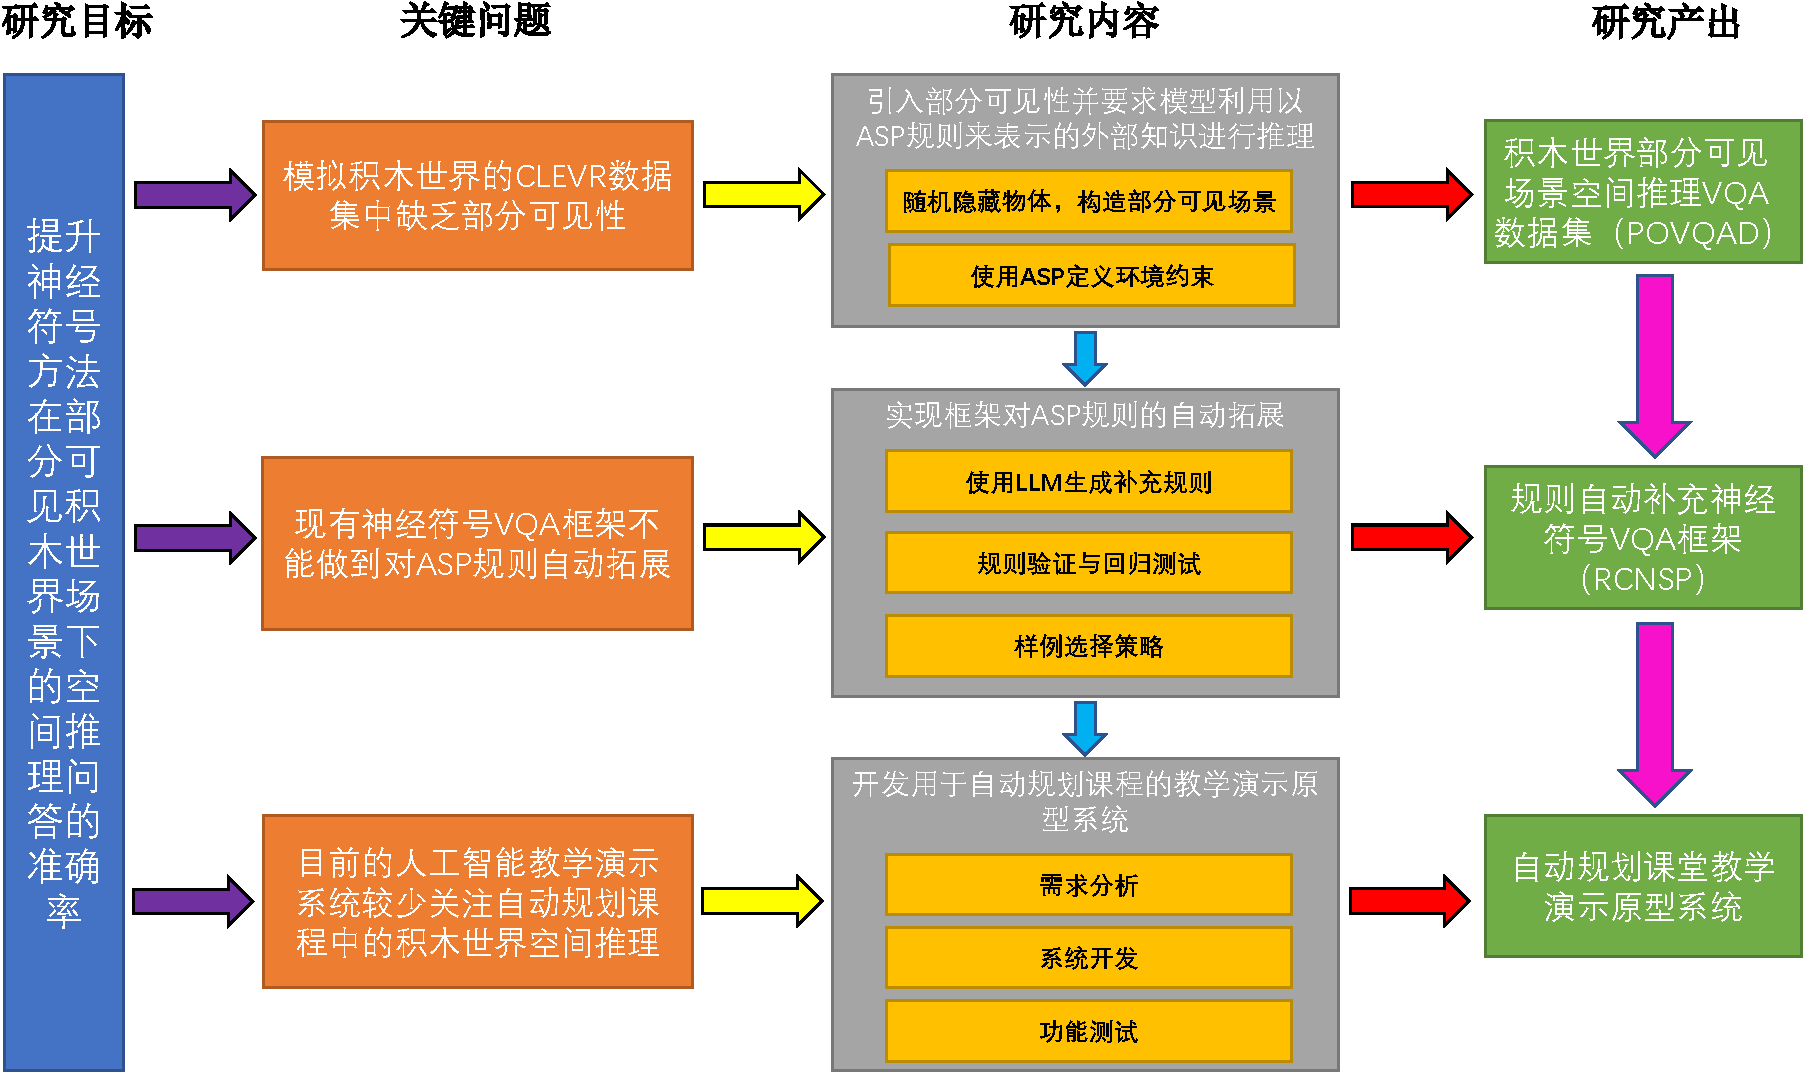
\includegraphics[width=\textwidth]{figures/research-guideline-crop.pdf}
    \caption{研究计划}
    \label{plan}
\end{figure}
% \begin{figure}[h]
%     \centering
%     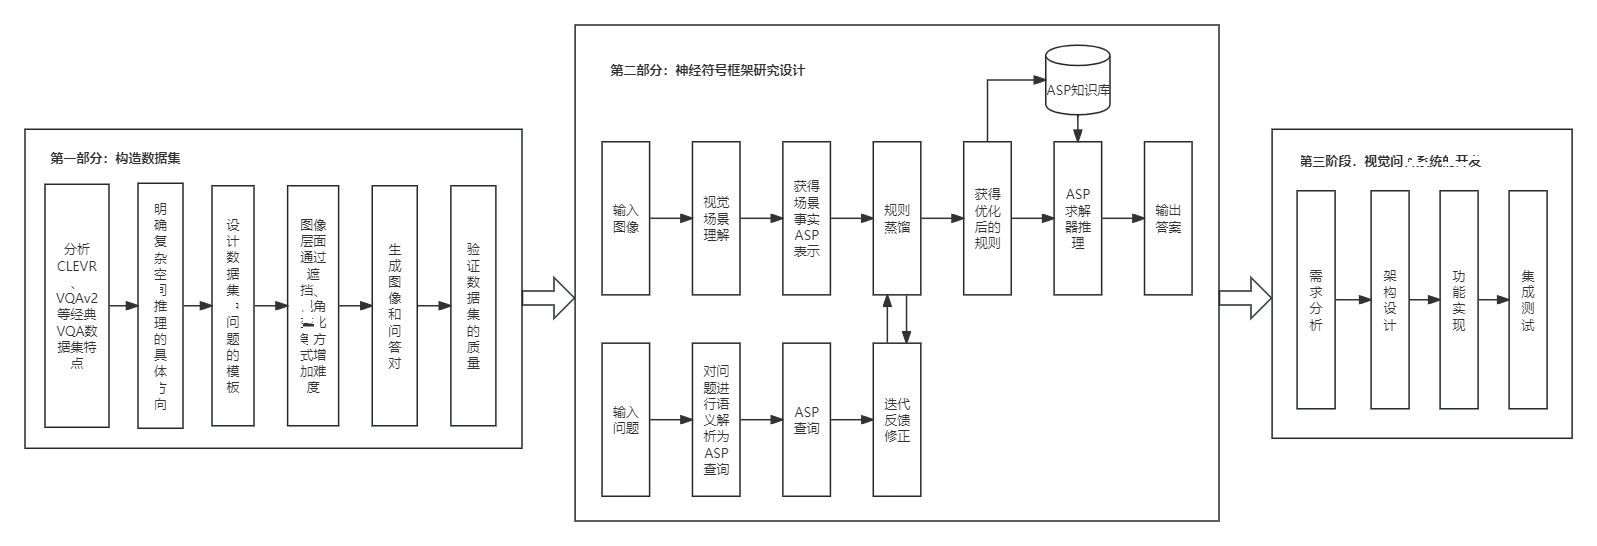
\includegraphics[width=\textwidth]{process.png}
%     \caption{技术路线图}
%     \label{roadmap}
% \end{figure}
\section{论文结构}
本文共分为六个章节,各章节的主要内容具体如下:

第一章为绪论,总体介绍本文的研究背景及意义、相关研究现状、研究思路及本文的结构安排。

第二章为背景知识,对本文涉及到的主要技术进行介绍,具体包括CLEVR数据集、ASP程序语法及ASP求解器、
GLIP以及DSPy。

第三章为数据集构建。对本文所用的视觉问答数据集进行详细介绍,
包括数据集的构造目的、数据集的研究方向、数据集的设计流程以及对数据集质量的验证。

第四章为神经符号VQA框架的研究设计。本章详细介绍本文设计的神经符号VQA框架,
包括总体架构、视觉场景理解、语义解析、知识蒸馏、迭代反馈、规则修正和 ASP 推理等模块,并通过对比试验证明了相比于VLM直接问答,神经符号方法能够有效提升模型在部分可见场景
下回答空间推理问题的正确率,并证明了本文新增的知识蒸馏模块能够进一步提升神经符号方法解决空间推理任务时的性能。

第五章为问答系统的设计与实现。对本文设计的VQA课堂教学演示原型系统进行详细介绍
,包括系统需求分析、系统架构设计、模块划分、模块实现和系统集成等内容。

第六章中对本文工作加以总结,分析本文的创新点和不足之处,并对未来的研究方向进行展望。


\input{chapter/Background.tex}

\chapter{POVQAD数据集构建}
\label{dataset}
本章旨在构建积木世界部分可见空间推理数据集,以便在后续研究中评估本文提出的神经符号VQA框架的性能,为本文的总研究目标服务。
下面分别就构建目标、构建准则、数据集定义、构建流程、数据集质量评估共五个方面展开介绍。
\section{构建目标}
本文提出构建一个积木世界部分可见场景空间推理数据集(Partial Observation VQA Data\-set, POVQAD)
,用于后续的研究中评估本文提出的神经符号VQA框架的性能。POVQAD的构建目标为:在部分可见积木世界场景下,通过遮挡、隐藏等设置,
考察模型结合背景知识和空间逻辑进行多步推理的能力。

以上数据集的构建目标,来源于以下几点:
\begin{enumerate}[nosep]
\item \textbf{CLEVR中场景信息完全可见}:对CLEVR中的某个问题而言,问题中涉及的所有物体,均在该问题对应的图像中
直接可见,不能反映现实世界中的部分场景可见的情形,不能满足本文研究目标中对于部分可见积木世界场景的需要。
例如,对于问题“What color is the cylinder to the left of the red sphere?”,
该问题对应的图像中左侧有一个蓝色圆柱体,右侧是红色球体。模型只需定位球体,并找其左侧物体,即可直接读取颜色。
\item \textbf{CLEVR缺少环境级逻辑约束}:CLEVR 场景中不存在“必须满足”的环境约束,
例如“所有红色物体必须是立方体”这类限制,使得推理任务缺乏积木世界空间推理中复杂性的模拟,不能考察模型综合利用背景知识进行系统推理的能力。
例如,对于问题“Are there more cubes than red things?”,
模型只需清点图像中立方体的数量和红色物体的数量即可比较并得出答案,而无需理解任何隐藏的逻辑条件或跨区域限制。
\item \textbf{CLEVR中问题的推理路径较短}:CLEVR中的很多问题只需一步推理或直接感知,不足以检验神经符号VQA框架在
积木世界多跳推理中的表现。例如,对于问题“What is the material of the small red object?”,模型只需要查找
图像中红色且尺寸为小的物体,即可直接回答材质,仅一次推理即可完成,推理路径很短。
\end{enumerate}
具体到数据集的各方面,构建目标可在图像、问题、环境约束、符号表示上进行进一步细化。
\subsection{图像层面目标}
图像层面上,具体包括以下目标:
\begin{enumerate}[nosep]
\item 设计部分遮挡和全遮挡两类图像。在实际VQA任务中,部分可见性是影响推理精度与鲁棒性的关键因素。
本文在构建POV\-QAD数据集时,特别关注两类具有代表性的“部分可见”情形——全遮挡图像和部分遮挡图像,并设计对应问题模板, 
以体现空间推理机制在不同可见性条件下的能力提升。

全遮挡图像属于“背景知识中已知,但图像中不可见”的情形。此类情形中,某些物体或其属性未出现在图像中,但依据环境布置的规则或先验知识,推理系统应当具备“补全”或“外推”能力。
例如:
\begin{enumerate}[nosep]
\item \textbf{背景约束}:场景中所有蓝色球体都放置在红色立方体后面,且每个红色立方体后面恰好有一个蓝球。
\item \textbf{图像内容(以文字描述)}:图中可见两个红色立方体,但它们后方区域被完全遮挡。
\item \textbf{问题示例}:这个场景中是否存在蓝色球体?
\end{enumerate}
尽管视觉输入中没有检测到任何蓝球,但根据背景规则和红立方体的数量,
系统应能得出“存在两个蓝球”的结论。这类问题强调的是利用背景知识进行结构性空间推理。

部分遮挡图像是“背景知识不足,且图像中被部分遮挡”的情形,这种情形代表了多数实际视觉任务中遇到的问题:
视觉系统可以检测部分被遮挡的物体,但缺乏对完整结构的观测,
难以仅靠视觉识别完成推理任务。本研究设计此类情境,旨在展示无需额外标注或监督,仅通过空间逻辑推理即可提升问答系统表现。例如:
\begin{enumerate}[nosep]
\item \textbf{图像内容(以文字描述)}:图中左侧有两个物体,其中一个绿色球体部分被另一个物体挡住,仅露出顶端。
\item \textbf{问题示例}:这个绿色球体是否位于红色立方体的上方?
\end{enumerate}
该情形下,仅凭部分视觉输入无法精确回答问题,但结合已有空间规则与遮挡顺序,系统可准确判断相对位置关系。
这类问题强调了空间逻辑推理在提升弱监督视觉问答中的作用。

因此,本文在POVQAD数据集中,特别设计了涵盖“背景知识可推理的完全不可见”和“无需标注即可推理的部分遮挡”两种部分可见情境,
以评估神经符号方法在复杂场景下的空间推理能力。
\item 保证高质量图像生成。本文设计的神经符号VQA框架中包含对图像的识别,需要根据识别出的物体以及物体之间的空间关系,
生成ASP规则以便后续针对不可见物体进行推理。因此能够准确、精准的识别可见的物体及其之间的关系,显得尤为重要,需要保证
图像以高质量水准生成,可见物体不能出现模糊、噪声等情况。
\item 将图像划分为多个区域。CLEVR没有对图像空间进行划分,不便于在空间层面定义一些约束条件,不能
充分考察模型的空间推理能力。通过将图像划分成若干个区域,可以将区域作为逻辑单元,便于定义局部或者跨区域的、全局的约束条件,验证
模型在空间层面上综合运用已有条件,进行逻辑推理的能力。
\end{enumerate}
\subsection{问题层面目标}
问题层面,具体包括以下目标:
\begin{enumerate}[nosep]
\item 以信息缺失物体为核心设计问题。CLEVR中的问题大多围绕图像中的完全可见的物体,即
回答该物体相关的问题的所需信息,全部都包括在图像中。CLEVR中的这一问题,导致CLEVR中缺少信息缺失的情境下的推理。
围绕信息缺失物体设计问题,可以引导模型进行推理、归纳,而非直接对图像进行感知并回答问题,考察模型的逻辑推理能力。
\item 控制问题类型分布。CLEVR中,物体的某些属性的问题的可能答案太少,例如关于材质的问题的可能答案仅有两种,
而颜色与形状的属性可取值较多,对应其相关问题的答案集空间更大,模型通过随机猜测命中的正确答案的概率大大降低。
故要对问题类型进行合理控制,尽可能扩大答案集空间,提高模型在“多值不确定性”下的能力。
\item 覆盖多种推理类型。CLEVR中的很多问题只需一步推理或直接感知,不足以检验神经符号VQA框架在
积木世界多跳推理中的表现。通过在POVQAD中设计不同推理跳数的问题,可以测试模型对链式逻辑的掌握程度。
\item 不直接通过“A在B的哪个方向?”这一类直接提问空间关系的问题,而是间接地设计问题来考察模型的空间推理能力。这一做法有以下几点原因:

(1)模拟真实场景中的不完全信息推理需求。在现实世界中,空间关系的应用经常是隐性的,不是直接问“哪个在左边”,而是:
“这个红球下面是什么?”或“最右边的立方体是什么颜色?”
但当部分场景不可见时,要想回答这类问题,模型就必须结合场景中已有的部分信息和环境约束进行空间补全和逻辑推理,
这实际上就考验了模型是否掌握了空间关系。而本文的问题中,目标物体(即被提问的物体)和参照物体(图像中信息完全,用来作为参照物的物体)
之间的关系均通过空间关系(上、下、左、右或者所在物体区域)来建立。如果要回答POVQAD中的问题,就必须要运用空间关系。

(2)防止模型直接记忆答案模式。如果问题中直接写明“左边的物体是什么”,模型可能只靠表面的模式学习就能答题,而不需要空间推理能力。
通过在问题设计上设置空间关系而不是直接提问,可以迫使模型“用上空间推理”而不是“看图找答案”。

(3)展现符号方法在空间推理方面的相对优势。本论文的研究目标之一是促进神经符号方法的发展。
直接提问空间关系可能会让纯神经模型也能勉强处理,而通过间接考察的方式,更有利于展现符号方法(如ASP)在空间建模方面的优势,
尤其是在显式表示空间约束、进行场景补全推理、得出结论的可解释性方面。
\end{enumerate}
\subsection{约束层面目标}
约束是对场景中对象空间配置的规则限制,定义对象之间的空间关系或位置要求。
每条约束基于一个约束模板实例化得到,具有明确的逻辑语义。
约束层面,具体包括以下目标:
\begin{enumerate}[nosep]
\item 使用ASP构建背景知识约束。CLEVR中对某个图像而言,缺少对其相关背景知识的设定,
进而无法考察模型是否能真正整合场景逻辑进行思考。而构建规则正是ASP的长处所在。
\item 模版化建模,支持约束组合多样性,形成多样化的环境。
CLEVR中。一方面对图像内物体数量、物体属性取值空间等要素均进行了参数化处理,可以自定义修改,另一方面支持多个模板之间的自由组合。
两种方法搭配,增加了环境的多样性。
\end{enumerate}
\subsection{符号表示层面目标}
符号表示层面的目标为:使用ASP进行统一编码。ASP是神经符号VQA框架的核心所在,在框架内部全程使用ASP进行知识表示,
能够有效减少不同知识表示形式之间进行转换而带来的损耗,保证知识的完整性。
\section{构建准则}
本文旨在构建一个部分可见积木世界场景的空间推理VQA数据集(POVQAD),用以模拟
现实世界中信息缺失的场景,并评估模型的空间推理能力。为实现该目标,本文在POVQAD数据集的构建中
遵循如下准则:
\begin{enumerate}[nosep]
\item 每个场景中有一个目标物体被隐藏,图像和逻辑表示中均不可见。场景指的是图像的ASP表示,其中包含了图像的物体属性及各物体之间的空间位置关系。
隐藏物体的目的是为了实现部分可见性,模拟现实中因遮挡或感知局限导致的信息缺失情境。
\item 每个场景都必须满足由 ASP 定义的一组环境约束,目的是保证场景内部在逻辑层面上的合理性,避免不同约束之间发生冲突。
例如,不能同时出现“区域1中所有物体都是蓝色”和“区域1中没有蓝色的物体”这种自相矛盾的约束。
\item 在环境约束定义、场景生成与问题的形式化表示方面,均采用ASP进行表示。原因在于以下几方面:

ASP支持高层次知识建模。POVQAD所涉及的空间推理任务,本质上是一个多层次的知识表示与约束求解问题。
环境约束定义了某类场景中物体属性分布的全局或局部规则;场景构建要求从这些规则中生成满足逻辑一致性的物体布局;
问题表示与求解则需要基于观察到的部分信息,反推出隐藏物体的属性。
在这些任务中,ASP具有以下核心优势:(1)声明式建模,使用逻辑规则直接描述“应该满足什么”,
而不是“如何计算”,避免编程过程的冗余细节;(2)非单一模型求解,ASP可自动求解所有满足条件的模型,天然适合多解推理任务;
(3)支持不完备信息建模,通过否定与缺省推理机制,可以有效表示部分可见性下的场景;
(4)可组合性强,环境约束、已知信息与问题查询均可通过逻辑程序合并输入,实现统一推理。

在环境约束生成中,ASP能够高效表达复杂的属性限制。环境约束可能包括限制属性取值(如“区域0中所有物体必须是红色或黄色”)、
限制物体数量(如“区域1中恰好有2个小物体”)、跨区域比较(如“区域1和区域2中相同颜色的物体数不能超过3”)以及
排他性限制(如“不得存在两个属性完全一致的物体”)。这些约束结构灵活,复杂度高,传统的数据生成方法难以精确表达。而 ASP 的规则语法(例如 :- 引入约束,\#进行计数等)非常适合表达此类逻辑条件。

在场景构建中,ASP可有效保障逻辑一致性。在场景构建过程中,ASP求解器被用作生成器,即在给定环境约束的前提下,
通过ASP求解器获得符合约束的场景。每个完整场景对应一组ASP事实;ASP求解器在物体属性组合与区域位置上
进行求解;最终仅保留满足所有约束条件的合法解集,用于渲染与问题生成。通过在场景构建中使用ASP求解器,
可以系统性地采样出大规模、逻辑一致、属性多样的积木世界场景,避免人工构造或启发式方法中可能出现的歧义与逻辑错误。

在问题表示中,ASP实现了可求解性与可解释性的统一。POVQAD中的问题不仅以自然语言形式存在,
还被转换为对应的ASP查询规则,这一方案的优势包括:(1)问题可直接嵌入ASP推理流程,与部分场景信息与环境约束统一求解;
(2)保证所有问题均具有可求解性:Clingo 求解器可验证其是否有合法答案;(3)通过分析解集大小、排除路径等,可进行问题难度分级与推理链可视化;
(4)每个问题的“答案空间”明确,适用于多解式评估与开放性回答。例如,问题“What is the color of the object with the same material as the object to the right of the red sphere?”可形式化为:
\begin{lstlisting}
query(Q) :-
  has_property(X, color, Q),has_property(X, shape, cylinder),
  has_property(Y, shape, sphere),has_property(Y, color, red),
  right(Y, X),same_material(X, Y),X != Y.
\end{lstlisting}
这种形式使得问题的语义清晰、结构明确,便于执行与验证。
\item 图像中物体属性设置形状、尺寸、材质、颜色四种属性。具体属性值的设置上,尺寸的可能取值为小、中、大,颜色的可能取值为红色、蓝
色、绿色、黄色、灰色、棕色、紫色和青色,材质的可能取值为橡胶和金属,形状的可能取值为圆锥体、球体、圆柱体和立方体。

选取这四种基本属性,是因为它们是物体最直观且容易区分的特征,并且与原始 CLEVR 数据集保持一致,便于进行比较研究。对
每个属性的可能取值进行了限制(例如,八种颜色,四种形状,两种材质,三种尺寸),
这样做的目的是为了简化推理过程并控制答案的搜索空间,避免由于可能的属性组合过多而导致的推理复杂度过高。
\item 图像中对空间进行划分,并分为四个区域,取值分别为0、1、2、3,并同时规定每个物体只能在图像的一个区域中,不能同时跨多个区域。
为图像空间划分区域,主要的优势在于为图像生成和问题生成指定作用范围约束,有利于提升数据集的复杂性和多样性。
\item 问题类型删除了CLEVR中的是否类问题(即比较属性、比较数量和存在性问题)以及计数问题,仅保留属性查询类问题。
做出这一规定的原因在于以下三点:

(1)POVQAD 的核心目标是评估模型在部分可见积木世界场景中进行空间推理的能力。
相比布尔值或数字作为结果的“是否类”与计数问题,
属性查询问题更能体现模型如何结合部分观测信息与环境约束,排除不符合条件的选项,最终推理出不可见物体的属性。

(2)是否类问题和计数问题的答案通常是“是/否”或整数,ASP 系统在求解这类问题时所涉及的推理路径较为简单
,缺乏中间可解释的逻辑链,难以体现复杂的空间推理过程。
而属性查询问题往往需要经过一系列基于已知信息的假设、排除、归纳等推理步骤,可以更完整地展现 ASP 系统的推理能力和可解释性。

(3)从实际教学与评估角度出发,属性查询问题有助于更好地分析模型失败的原因,
便于定位是视觉理解错误、知识调用缺失,还是逻辑链条断裂;而布尔类问题的回答更难反推推理过程中的缺陷。

因此,为更精准地衡量模型在复杂空间推理任务中的表现,并提升神经符号方法的可解释性与诊断性,本文在 POVQAD 中仅保留属性查询类问题。
\end{enumerate}
\section{数据集定义}
基于上述构建目标,本文将POVQAD数据集形式化定义为一个五元组的集合:
$$D = \{ (I_i,P_i,Q_i,\Pi_i ,A_i) | i=1,2,...,N \}$$
其中,每个元素$(I_i,P_i,Q_i,\Pi_i ,A_i)$是数据集中的一个样例,各组成部分定义如下:
\begin{enumerate}[nosep]
\item \textbf{$I_i$}为图像,是通过 Blender 渲染的基于场景生成的 3D 图像。
每张图像表示一个三维积木世界场景,所有可见物体均按预定义属性摆放。每个图像中都刻意隐藏了一个物体,以模拟部分可见条件。
图像示例如图\ref{POVQAD-figure}。
\begin{figure}
\centering
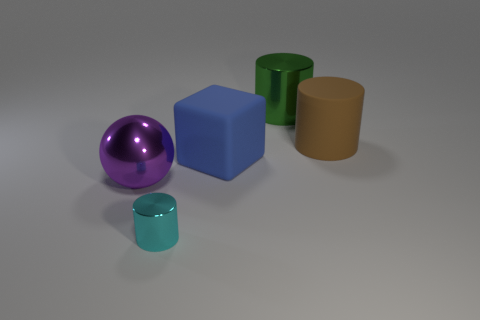
\includegraphics[scale=0.6]{figures/POVQAD中图像示例.png}
\caption{POVQAD中图像示例}
\label{POVQAD-figure}
\end{figure}
\item \textbf{$S_i$}为场景,是对当前图像中所有可见物体的ASP表示,采用ASP进行表示。
其中主要包含以下内容:每个可见物体的属性,包括尺寸、颜色、材质、形状;每个物体所属的区域;可见物体之间的空间关系,如\textbf{left(X,Y)}表示X在Y的左边;
被隐藏的物体(即问题中提及而图像中不存在的物体)不会出现在部分场景信息中。
\item \textbf{$Q_i$}为问题,使用自然语言形式进行表示,例如“What shape is the small red object that is to the left of the yellow cube?”。
所有问题均为属性查询类问题,专门针对物体的四个属性之一:颜色、尺寸、形状或材质。
\item \textbf{$QA_i$}为问题的ASP表示,例如:
\begin{lstlisting}
query(Q) :-
  has_property(X, color, Q),has_property(X, shape, cylinder),
  has_property(Y, shape, sphere),has_property(Y, color, red),
  left(Y, X),same_material(X, Y),X != Y.
\end{lstlisting}
\item \textbf{$\Pi_i$}为环境,是当前图像所属环境的一组约束规则,采用ASP进行表示。以下为一组约束示例:
\begin{lstlisting}
% 约束示例
% 区域0中所有物体的形状必须是圆柱体
:- obj(X), at(X, 0), has_property(X, shape, cylinder).
% 区域1中蓝色物体的数量大于2个
:- #count{X: has_property(X, color, blue), at(X, 1)} > 2.
\end{lstlisting}
\item \textbf{$A_i$}为答案集,表示该问题对应的正确答案。
\end{enumerate}
\section{构建流程}
POVQAD的构建流程如图\ref{fig:dataset-generation}所示,共包括5个步骤。各个步骤的功能如下:
\begin{enumerate}[nosep]
\item \textbf{生成环境}:随机选取部分约束模板,并将模板实例化,最终得到环境。
\item \textbf{构建场景图}:将环境实例化,并将环境输入ASP求解器进行求解,分别生成部分可见场景图和不可见场景图。
\item \textbf{图像渲染}:使用Blender对场景图进行渲染,获得积木世界图像与场景。
\item \textbf{问题生成}:根据问题模板与场景生成问题与其对应ASP查询,并使用Clingo得到问题的解,此外对答案集进行筛选。
\end{enumerate}
\begin{figure}[h]
\centering
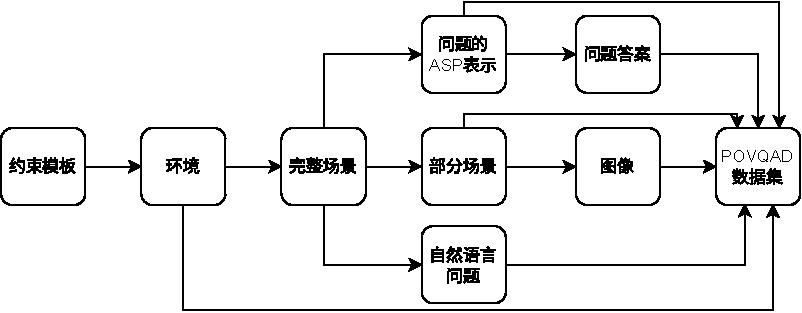
\includegraphics{figures/pipeline-POVQAD.drawio-crop.pdf}
\caption{POVQAD构建流程}
\label{fig:dataset-generation}
\end{figure}

\subsection{生成环境}
在POVQAD中,一个环境包含了一组约束规则,用于限定在该环境下生成的所有场景所必须满足的
属性组合、区域位置的约束条件。环境的作用是,在宏观层面上对后续生成的图像、问题进行把控,
以控制场景复杂度,并保证数据集保持逻辑一致性。在数学上可以如下表示环境:
$$ \varepsilon = \{C_1,C_2, ..., C_k \}, C_i \in ASP \quad Constraint $$
其中,每个$C_i$是用 ASP 表示的一条逻辑约束规则。

环境的生成过程包括以下步骤:(1)预定义11种约束模板;(2)确定模板中的相关参数;(3)对所有生成的约束经语义检查与逻辑一致性验证。

约束模板是依据常见的逻辑组合来进行设计的,覆盖了取值限定、逻辑否、逻辑或等基本逻辑模式,
部分约束模板的ASP编码表示以及对应表示含义见表\ref{tab:asp_templates},全部约束模板见附录\ref{appendix:constraints}。
除了约束模板之外,还有全局约束。
全局约束是所有生成的环境都应遵循的约束,对整个积木世界进行了基本定义,例如“平面区域划分为4个,编号0、1、2、3。”就是通过全局约束定义的,
ASP形式为\texttt{region(0). region(1). region(2). region(3).}。
本文所用的所有全局约束在附录\ref{appendix:environment}同样予以了展示。
\begin{table}[h]
    \centering
    \renewcommand{\arraystretch}{1.0}
    \begin{tabular}{|p{2.8cm}|p{12.2cm}|}
        \hline
        \textbf{模板} & \textbf{描述} \\
        \hline
        \textbf{模板1(取值约束)} & 
        \texttt{:- obj(X), at(X, R), not has\_property(X, P1, V1).} \\ 
        & 解释: 对区域R中的所有物体,它们P1属性的取值均为V1。 \\ 
        & 具体实现: :- obj(X), at(X, 0), not has\_property(X, color, red). \\
        \hline
        \textbf{模板2(遮挡比例约束)} & 
        \texttt{:- occlusion\_rate(T, R), (R <= 0; R >= 1).} \\ 
        & 解释:物体T被遮挡的比例为R(0<R<=1),完全遮挡时R=1。 \\ 
        & 具体实现::- occlusion\_rate(T, 0.1). \\
        \hline
    \end{tabular}
    \caption{部分约束模板示例}
    \label{tab:asp_templates}
\end{table}

模板实例化生成环境的过程中,需要设定一些参数,具体包括:
\begin{enumerate}[nosep]
\item \textbf{规则模板数量}:每个环境实例化多少条规则模板,规定单个环境最多实例化15条。
\item \textbf{属性类型}:将模板中的属性类型占位符用实际生成的属性类型进行替换,例如 P1' 替换为 color,P2' 替换为 shape。
\item \textbf{属性值}:用随机生成的属性值替换,例如 V1' 替换为 red,V2' 替换为 sphere。
\item \textbf{区域范围}:规则作用在哪些区域。根据POVQAD的定义,区域编号为0、1、2、3。
如果是全局作用的模板,则需要将该条规则的作用区域设置为0、1、2、3。如果是作用在局部区域,仅需设置某个或某几个区域即可。
\item \textbf{数量参数}:恰有、至少、至多约束中要求的具体数量。
\end{enumerate}

模板实例化之后,再基于所得的模板实例,为每个区域生成区域内约束,并随机生成跨区域约束和强制否定约束。
强制否定约束用于限制某些属性或者属性做个不能出现在特定区域中,跨区域约束用于限制多个区域之间对象的关系或者属性分布,区域内约束
用于限制单个区域内对象的属性或者属性组合。
最终,得到具体的约束表达式如下所示:
\begin{lstlisting}
:- object(X), at(X, 0), not hasProperty(X, color, red).
:- object(X), at(X, 1), hasProperty(X, shape, cube).
:- #count{sameProperty(X1, X2, color): object(X1), object(X2), at(X1, 0), at(X2, 1)} < 2.
\end{lstlisting}

POVQAD规定每个环境最多由15条约束规则模板实例化构成,这一数值是经过多方面权衡确定的,目的主要在于以下几方面:
\begin{enumerate}[nosep]
\item 逻辑复杂度与可解性的平衡。如果某个环境中的约束规则过少,会导致后续生成的场景过于松散,
物体属性组合高度自由,推理空间过大,导致问题复杂度过大,难以进行有效推理。
如果约束规则过多,则会造成约束之间产生冲突,导致ASP求解器难以知道合法的解,影响求解效率,进而影响场景的生成。
\item 控制生成时间与可维护性。每条规则在 ASP 中都可能极大影响解空间,规则数上升将显著增加 ASP 求解时间。此外,
在大规模数据生成中,15 条以内的环境可以在数秒内稳定求解出场景,利于批量生成和调试。
\end{enumerate}

在生成环境的过程中,规定每个环境中至少包括区域级约束和跨区域约束,共计两种约束。做出这一规定的目的在于
增强环境的逻辑层次性与推理深度,具体原因如下:
\begin{enumerate}[nosep]
\item 支持多层次推理链的构造。区域级约束用于构建局部一致性,跨区域约束用于建模全局对比或协同关系。
同时使用这两类约束,可以使推理问题具有从局部到跨区域的空间层级,增加问题的空间深度。
\item 避免场景构造退化为简单的组合。如果只使用区域级约束,那么后续根据环境生成场景时,将会变成多个局部区域的简单组合,
缺乏各个区域之间的相互关联。添加跨区域约束之后,有助于生成具有全局一致性/相互限制/相互支撑的复杂场景。
\item 支撑部分可见场景下的间接推理。在部分场景中,若不可见物体在区域0中缺失,模型可以通过区域0的其它规则
或者区域0与区域1的对比或者联动规则来进行属性排除或依存判断。而如果采用单一的区域级约束,
那么对于区域0中的物体的问题,模型只能依赖于区域0的局部信息进行推理,缺乏全局视角,不利于考察模型的宏观层面推理能力。
\end{enumerate}

此后在生成环境时,将全局约束与获得的约束表达式进行拼接,形成完整ASP程序,并由Clingo对ASP程序进行求解。
如果Clingo的输出至少存在一个答案集,说明当前约束可满足,将所得结果(即环境)保存到ASP程序的\texttt{.lp}文件中。如果Clingo没有答案集,说明当前约束不满足,会
尝试使用其它的约束表达式进行求解,直到能够生成一个环境。

进行语义检查与逻辑一致性验证的具体方案是用ASP求解器(本文中采用Clingo)对生成的约束尝试进行求解,
如果Clingo没有提示错误信息,并且能够成功求解出至少一个合法的解集,则说明该环境的约束规则是逻辑一致的,并且
能够顺利通过语法检查。本步骤的主要目标是避免后续出现死循环、空解等问题。

最终,一共生成了30个环境,数据集中的所有场景均匀分布在这些不同的环境之中。
控制生成30个环境的原因是,这一数量的环境实际上可以供后续生成数百万个不同场景和问题,足够支撑进行大规模训练与严格测试。
环境的具体示例见附录\ref{appendix:environment}。
\subsection{构建场景}
\subsubsection{构建完整场景图}
在获得环境约束后,需要进一步获得符合约束的场景图,所需流程为:
将获得的环境约束Clingo进行求解,生成符合约束的答案集,并对答案集进行采样。一个答案集
对应一个完整场景图。此后,将答案集进行解析,获得完整场景图。

首先,将包含了环境约束的\texttt{.lp}文件提交至Clingo进行求解,对Clingo的输出结果进行简单解析,将所有答案集进行提取。

在生成答案集之后进行采样出于以下两点原因:
\begin{enumerate}[nosep]
\item 避免处理过多的答案集。如果直接处理所有答案集,会导致后续的场景生成和问题生成过程耗费大量时间和资源。
\item 控制场景的多样性。如果直接使用所有答案集,可能会生成大量相似的场景,导致数据集的多样性不足。
某些约束可能会导致生成的场景具有高度重复的物体属性或关系。随机采样可以增加场景的多样性,避免生成过于相似的场景。
\item 平衡约束类型的答案集。不同的约束类型可能会生成不同数量的答案集。
如果某些约束类型生成的答案集过多,而其他约束类型生成的答案集较少,可能会导致数据集中某些类型的场景占比过高。
对每种约束类型的答案集进行采样,可以平衡不同约束类型的场景数量,确保数据集的均衡性。
\item 降低后续处理的复杂度。每个答案集需要进一步解析为场景图,并用于生成图像和问题。
如果答案集数量过多,会显著增加后续处理的复杂度。通过减少答案集数量,降低后续处理的复杂度,确保生成管道的可控性。
\end{enumerate}

场景是最终渲染的图像及其对应的描述信息,包括图像中的所有物体及其属性和位置。场景以JSON文件存储,某个场景如下所示:
\begin{lstlisting}

\end{lstlisting}

场景图是场景的结构化表示,描述了场景中物体的属性以及物体之间的关系,是场景的一种中间表示。某个场景图如下所示:
\begin{lstlisting}
{
  0: {"color": "red", "shape": "sphere", "size": "large", "material": "rubber", "region": 0},
  1: {"color": "blue", "shape": "cube", "size": "small", "material": "metal", "region": 1}
}
\end{lstlisting}

对答案集进行解析的过程实际上是对谓词进行解析的过程,会将\texttt{has\_property}和\texttt{at}两个谓词进行解析,
最终形成以JSON格式存储的场景图。

此后基于所得的完整场景可以生成部分可见场景和不可见场景。以下两小节将展开介绍。
\subsubsection{构建部分可见场景图}
部分可见场景与完整场景的区别在于:部分可见场景中增加了对于物体之间遮挡关系以及遮挡比例的规则,进而后续Blender根据场景
渲染图像时,能够得到场景中描述的部分物体之间存在遮挡的图像。构建部分可见场景的具体流程如下:

首先从完整场景中,随机选取两个物体,并分别指定一个物体为将会被提问的目标物体\texttt{T}
,另一个物体为去遮挡目标物体的\texttt{Oc}。
此后,向场景中添加ASP谓词\texttt{target(T)}、\texttt{occluder(Oc)}以及\texttt{occludes(Oc,T)},分别表示
\texttt{T}为目标物体,\texttt{Oc}为遮挡物体,Oc在图像中遮挡了T。此后,生成一个介于0和1之间的随机数$R$,用于表示目标物体
被遮挡的面积比例。本文规定$R$大于0且小于1。当$R=1$时,相当于目标物体被完全遮挡,对应不可见场景的构建,为其它不同的构造方法。

此后,再随机选择目标物体\texttt{T}的形状、颜色、材质、尺寸中的任意一个属性,将其从场景中移除,以表示由于该物体被遮挡导致的信息缺失。
\subsubsection{构建不可见场景图}
基于完整场景构图建不可见场景图的构造思路是:从完整场景图中随机移除一个对象。

本环节的目标是,从完整场景中随机选择一个物体作为被隐藏的目标物体,并围绕该物体构造相关问题
,并同时使用自然语言及ASP对问题进行表示。
整个环节的流程图如\ref{generate-partial-scenes-and-questions}所示。
\begin{figure}[h]
\centering
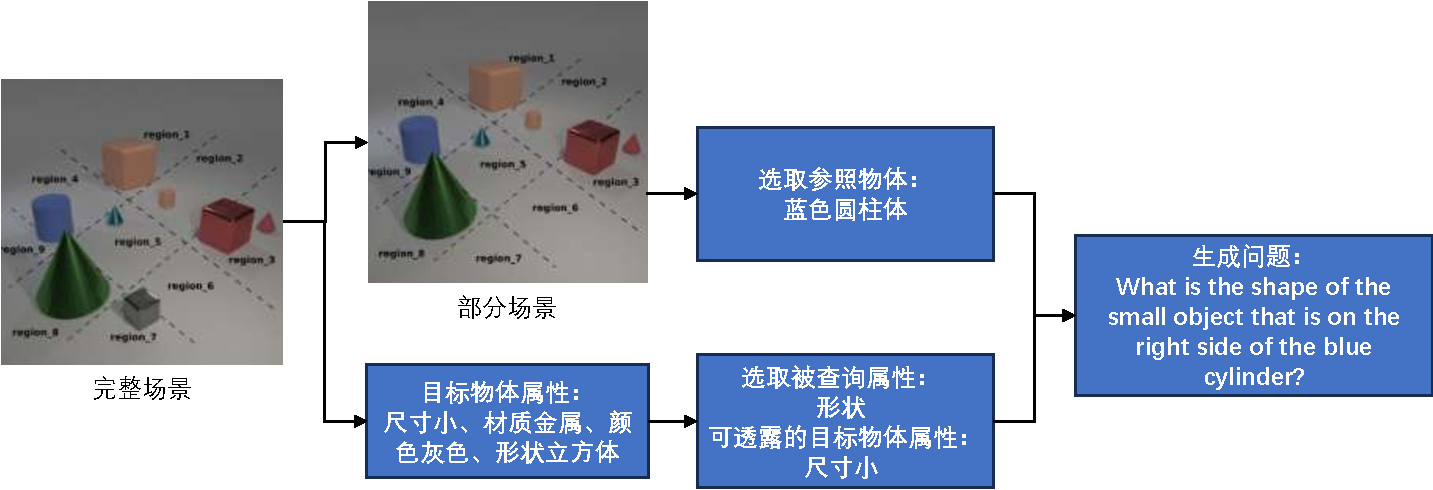
\includegraphics[scale=0.6]{figures/部分场景及问题生成-crop.pdf}
\caption{构建部分场景并生成问题流程图}
\label{generate-partial-scenes-and-questions}
\end{figure}

选择目标物体的过程需要满足以下条件:
\begin{enumerate}[nosep]
\item 从完整场景的所有物体中随机选取一个,在随机选取的过程中,要注意保持均衡,不能
一直选取单一区域的物体或者相同属性的物体,以免造成数据偏态分布。
\item 被选择物体不能是唯一出现某一属性的对象,避免由于移除该物体后,
导致场景中该属性的值无法被推断,导致问题无解。
\item 该物体将在后续问题中作为查询目标。
\end{enumerate}

选择$Obj_i$后,需要将完整场景中关于$Obj_i$的所有事实全部移除,生成部分场景。具体需要做到以下几点:
\begin{enumerate}[nosep]
\item 删除\texttt{obj(i)}、\texttt{at(i, R)}、\texttt{has\_property(i, P, V)};
\item 删除所有涉及$Obj_i$的空间关系谓词,如\texttt{left(i, j)}、\texttt{right(i, j)}等;
\item 保留其余物体的信息与关系。
\end{enumerate}
从而得到一个只包含可见物体的子结构,记为 $Partial_i$,该场景中缺少了目标物体的显式信息。

随后,将根据$Obj_i$的属性来生成相关问题。
每一个生成的问题,应该满足如下条件:(1)针对被隐藏对象的某一属性;
(2)基于剩余可见物体和环境约束进行间接推理;(3)问题语义必须明确且答案集非空。
以某个问题的生成为例,$Obj_i$的属性包括:尺寸为小、材质为金属、颜色为灰色、形状为立方体
,那么可以随机选取形状作为被查询属性,并将“尺寸为小”作为已知信息放置在问题当中。
为了便于控制问题类型的数量分布,本文规定每个问题只能查询上述四个属性中的一个,而不同时查询多个属性。
与此同时,问题生成器也将从图中选取一个
参照物体,用以共同组成问题。考虑到不同种类属性的可能取值数量不同,进而不同属性的问题的可能答案数量也不同,
本文据此规定每种属性的问题在数据集中所占的比例:颜色与形状各占40\%,材质与尺寸各占10\%。
该比例同样通过ASP约束来进行实现。
需要注意生成的问题仅为属性查询问题,不包括是非题和计数题等其它CLEVR中原有的问题类型,理由在3.1节构建目标中已有陈述,此处不再赘述。

\subsection{图像渲染}
图像渲染与样例生成的目的是将部分可见场景图以及不可见场景图转换为场景,并使用Blender进行渲染。

\begin{enumerate}[nosep]
\item 初始化Blender渲染对象。在这一步中,主要是设置一系列渲染参数,包括分辨率、GPU设置等等。
\item 定义场景字典。该字典中保存了场景的元信息(即将生成的图片名称等)、物体信息和方向信息。
\item 方向向量计算。先获取在场景初始化时添加的平面的法向量,此后计算摄像机的方向向量,并将
摄像机的方向向量投影到平面上,得到相对于平面的方向向量。计算完成之后,将平面删除,避免影响后续渲染
\item 向场景中添加物体。根据场景图中的物体信息,将物体添加到场景中。添加过程中,要注意确保物体之间的距离和边距满足约束条件。
此外,在生成部分可见场景时,要注意根据部分可见场景图中的遮挡物体和遮挡面积比例,来生成遮挡的情形;
在生成不可见场景时,要注意。
\item 计算物体之间关系。基于物体的三维坐标和场景的方向向量,遍历场景中的每对物体,
计算得出空间中上、下、左、右、前、后等关系。判断两个物体之间是否存在某种关系的阈值设置为0.2,即如果两个物体之间的
方向向量的点积大于0.2,那么认为它们具有该关系。

最终,输出一个JSON对象,其中描述了场景中所有物体之间的空间关系,一个可能的字典如图所示,其中$left[0] = 1$说明
物体0的左侧有物体1,$right[1] = 0$说明物体1的右侧有物体0。
\begin{lstlisting}
{
    "left": [[1], [], [], []],
    "right": [[], [0], [], []],
    "above": [[], [], [3], []],
    "below": [[], [], [], [2]],
    "front": [[], [], [], []],
    "behind": [[], [], [], []]
}
\end{lstlisting}
\end{enumerate}

在图像渲染完成之后,整个场景构造完成,此时进行数据整合,将所有场景文件合并同一个包含所有场景的JSON文件中。

\subsection{问题生成}
POVQAD根据前述步骤整合的场景文件和问题模板来构造自然语言问题,
一种供参考的模板如\ref{asp:question-template}中所示,
其中<Z2>、<C2>、<M2> 表示待查询对象的已知属性(例如尺寸、颜色、材质),由随机策略从完整场景中选取;
<R> 为空间关系(如left、right、front、behind),其取值既满足随机性,又依赖于完整场景中物体间的真实空间分布;
<Z>、<C>、<M>、<S> 则代表参考对象的属性。这种模板化设计不仅使自然语言问题的结构化描述成为可能,
而且便于后续转换为ASP的形式化表示,从而实现问题求解的自动化。
\begin{lstlisting}[label=asp:question-template]
What shape is the < Z2 > (size) < C2 > (color) < M2 > (material) [that is] 
< R > (relation) the < Z > (size) < C > (color) < M > (material) < S > (shape) ?
\end{lstlisting}

首先,筛选问题模板。对模板的筛选,按照模板的查询目标是否与当前场景相匹配,以及模板中给定信息是否在场景中存在来进行。例如,对于下列问题模板,其提问的是
“物体A是否在物体B的上方?”但是该场景图中,两物体之间的
\begin{lstlisting}

\end{lstlisting}

问题模板筛选完毕之后,根据场景图和筛选好的问题模板,进行模板实例化,生成问题文本及其对应的ASP查询。
实例化过程中,需要对模板中的占位符替换为具体的属性值。对每一个自然语言问题,都是从一个问题模板出发,填充占位符,
然后生成的。所以,自然语言和ASP查询具有一一对应的逻辑结构,可以实现自动转换。

此后调用Clingo求解查询,生成问题的答案,并通过对答案进行分析,实现对生成问题的筛选。
筛选逻辑是:如果答案集为空或者包含所有的可能值,则丢弃当前问题。对生成问题进行筛选有以下三点原因:
\begin{enumerate}[nosep]
\item 提高问题的质量。确保生成的问题有明确的答案,而不是模糊或无意义的问题。
\item 避免冗余问题。避免生成答案集过大的问题,这些问题可能对模型训练没有帮助。
\item 确保问题的多样性。筛选掉覆盖所有可能答案的情况,确保问题具有一定的区分性。
\end{enumerate}

最后,将生成的问题、ASP查询和答案保存为JSON文件,以下为一个示例:
\begin{lstlisting}
{
    'split': scene_info['split'],
    'image_filename': scene_fn,
    'image_index': image_index,
    'question': ts,
    'program': qs,
    'asp_query': asp_query,
    'answer': possible_sols,
    'object_interest': obj_interest,
    'template_filename': fn,
    'question_family_index': idx,
    'question_index': image_index
}
\end{lstlisting}

\section{数据集质量评估}
为验证构造的POVQAD数据集的可靠性与研究价值,本节从POVQAD的可执行性与一致性、统计分析、对比实验方面进行研究。
\subsection{可执行性与一致性评估}
可执行性指的是POVQAD中每个样例的ASP程序能够经Clingo求解器执行,不出现语法错误。
一致性指的是对POVQAD中每个样例的ASP程序,Clingo对其的求解结果与样例中给出的标准答案一致。

本文对POVQAD中所有ASP程序依次使用Clingo进行执行,统计语法错误率,结果为0.2\%,
并且对能够正确执行的ASP程序的运行结果与标准答案进行对比分析,一致率为99.5\%,以上两点证明本文生成的ASP程序质量较高,
使用ASP构造POVQAD的方法合理。
\subsection{统计分析}
POVQAD中问题分布的统计图见图\ref{fig:question_statistics}。从图\ref{fig:question_statistics}(a)中可得知,有关颜色和形状的问题在POVQAD数据集中
占比最高,分别是39\%和37.6\%,关于大小和材质的问题则相对较少,分别只占到了13.6\%和9.8\%。
所提问题的类型取决于被查询的物体的属性,在生成数据集的过程中,允许用户设置问题类型的预期占比。
以上统计得到的POVQAD中问题类型占比,是基于以下的设置生成的:颜色问题占比40\%,形状问题占比40\%,大小问题占比10\%,材质问题占比10\%。
做出如上设置的原因是,与材质(只有两个值)相比,颜色和形状等属性包含更大的值集合(颜色有 8 个值,形状有 4 个值),
则对颜色和形状提问的问题有更多的潜在答案,故应将颜色和形状的相关问题的占比调高,以充分展示相关问题的答案集空间。

图\ref{fig:question_statistics}(b)、(c)、(d)和(e)分别说明了各种问题类型(尺寸、形状、材质和颜色)的潜在答案的分布。
生成数据集的目标之一是实现均衡的分布,避免大多数问题都导致相同的答案集的情况。
例如,当问题涉及物体的大小时,其可能的解可以是
 \{大, 中\}、\{大, 小\}、\{小, 中\}、\{大\}、\{中\} 或 \{小\} 之一,
 如图\ref{fig:question_statistics}(b)所示。由于查询属性为颜色的问题的可能答案数量很大(因为颜色可以取 8 个值),
 因此图\ref{fig:question_statistics}(e)中并未列出整个空间。根据统计图可以看出,在生成过程中没有偏向任何特定的答案。
\begin{figure}[h]
    \centering
    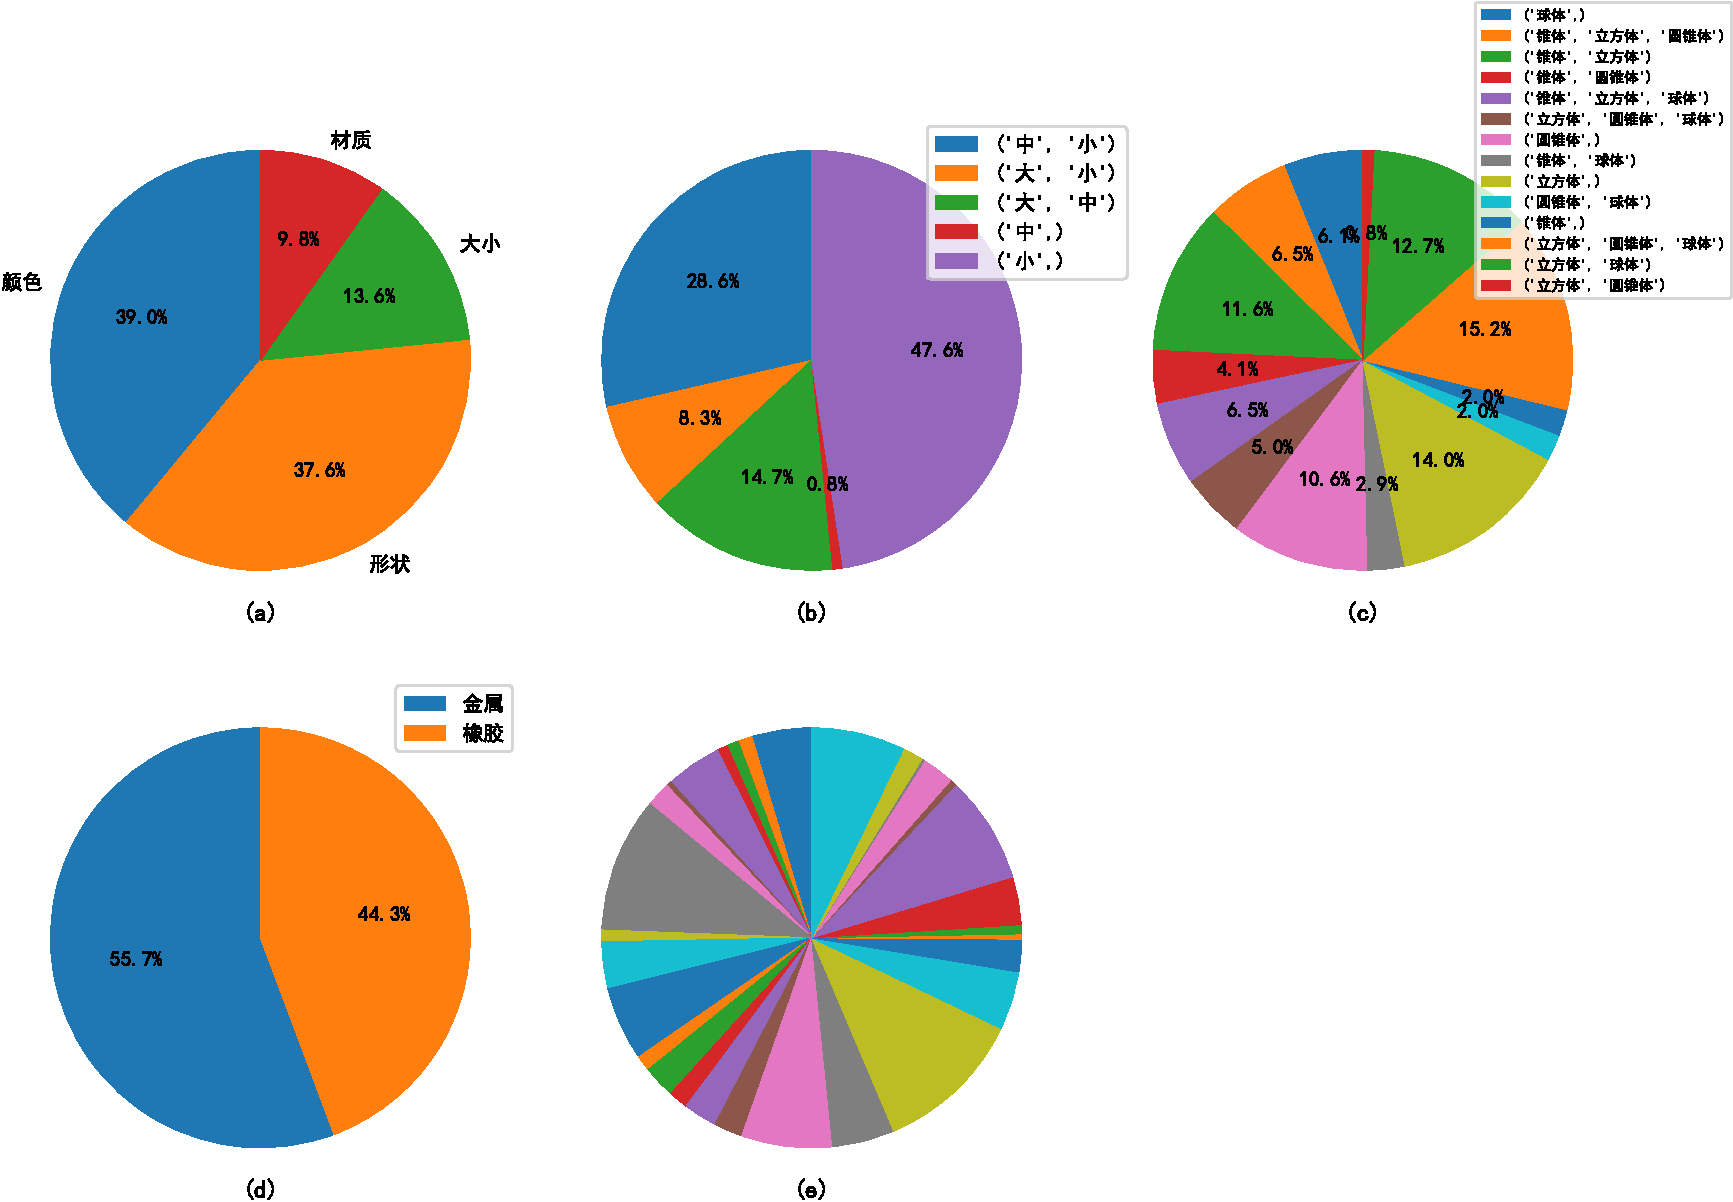
\includegraphics[scale=0.45]{figures/question_distribution-crop.pdf}
    \caption{问题分布统计}
    \label{fig:question_statistics}
\end{figure}

图\ref{fig:template_statistics}(a)中展示了POVQAD中问题在不同问题模板上的分布情况,\ref{fig:template_statistics}(b)中展示
了特定类型问题根据场景中物体数量划分的分布情况。
\begin{figure}[h]
    \centering
    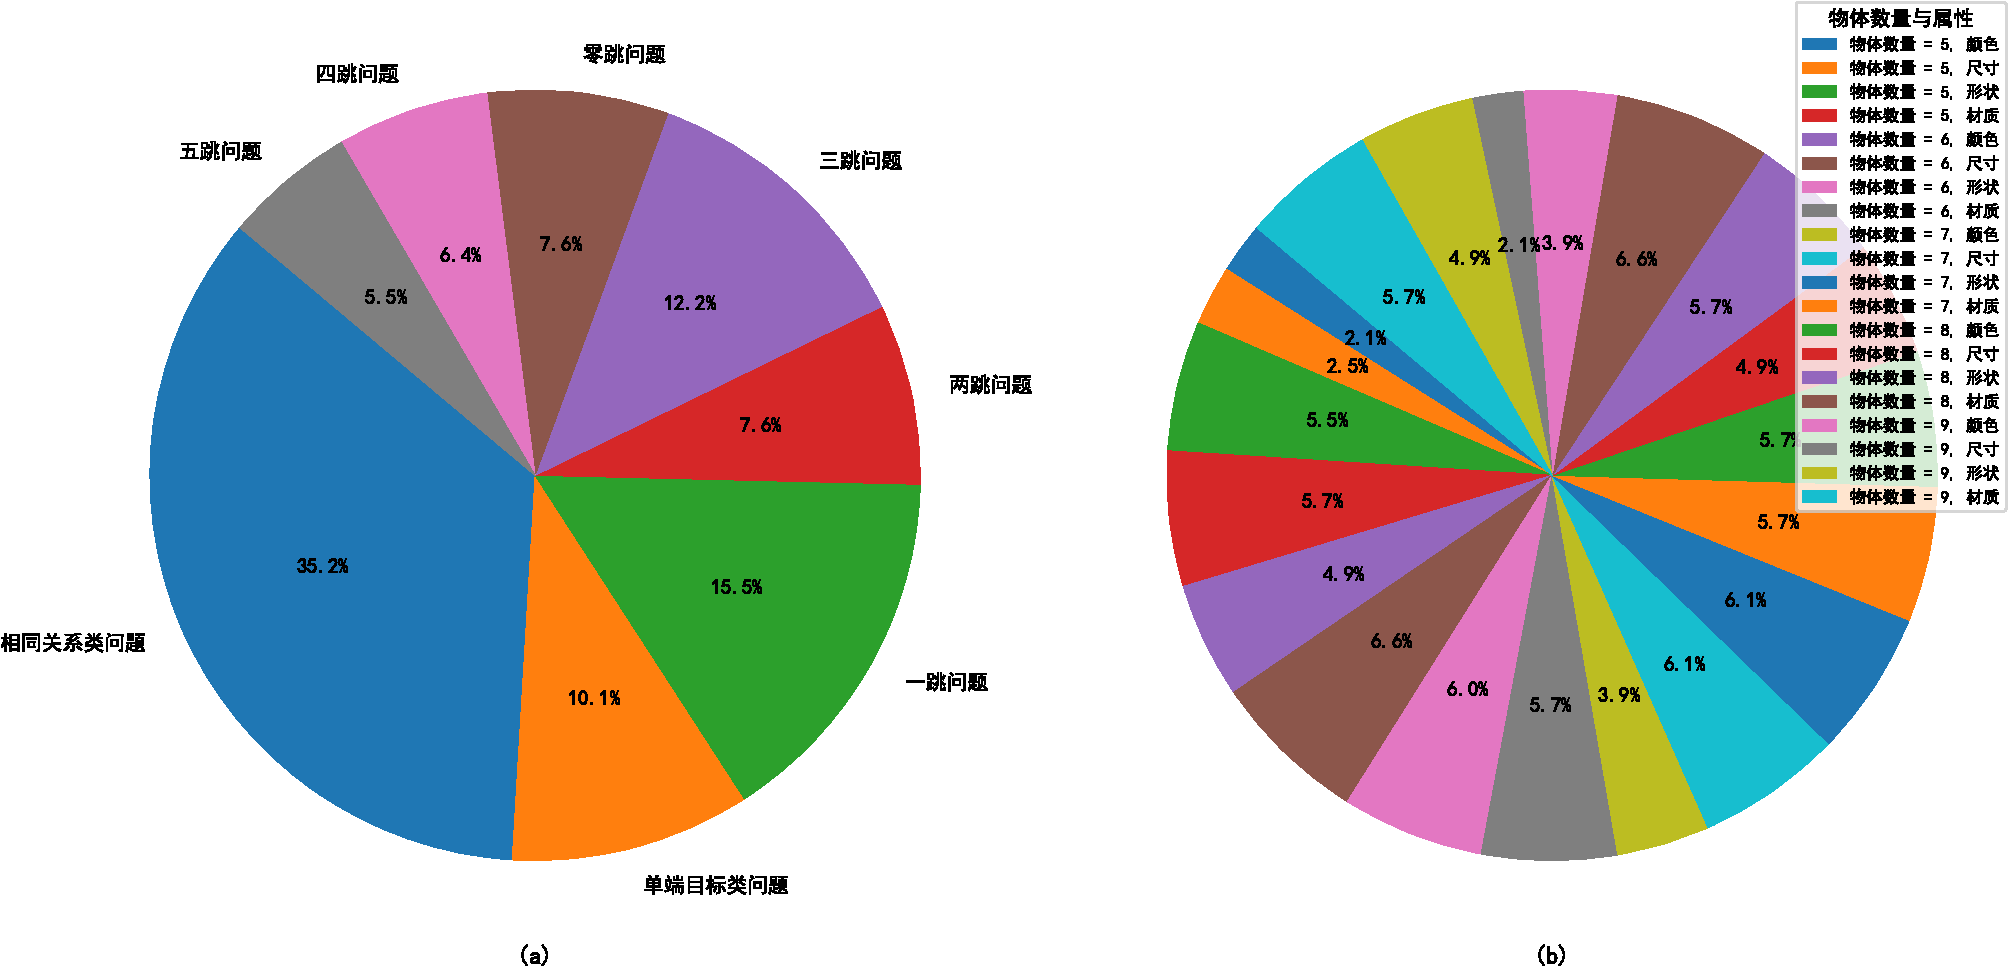
\includegraphics[scale=0.45]{figures/question_template_distribution-crop.pdf}
    \caption{问题模板分布情况}
    \label{fig:template_statistics}
\end{figure}
\subsection{对比实验}
为了证明POVQAD数据集对不同推理能力方法的区分性与挑战性,
本文选取了五种代表性方法在该数据集上进行实验:传统感知模型(CNN+LSTM)、
主流多模态大模型(DeepSeek、Gemini 2.5 Flash、ChatGPT-4o),以及人类作答作为理论上限参考。
每种方法的输入为POVQAD的图像、自然语言问题以及环境约束。实验重复进行三次取平均值,最终实验结果如图\ref{fig:dataset-comparison}所示,可得出如下结论:
\begin{enumerate}[nosep]
\item 数据集具有良好的难度区分能力。各方法在POVQAD上的准确率差异明显,充分体现了模型间的空间理解与逻辑推理能力差距。尤其是传统模型(CNN+LSTM)仅达到 45.4\% 的准确率,明显低于VLMs方法,显示POVQAD对浅层感知模型构成了挑战。
\item 多模态大模型在不完全信息推理方面存在性能瓶颈。
即便是先进的多模态大模型(如 ChatGPT-4o)也未能达到人类水平,
在复杂场景、信息遮挡和规则约束下的准确率仍有明显提升空间,说明POVQAD能有效考察模型对隐含信息与环境规则的建模能力。
\item POVQAD能作为更强推理任务的评估基准。
结果表明,POVQAD能有效区分浅层感知模型与具备显式推理机制的方法,
同时能检测当前主流多模态模型在空间推理与知识补全方面的能力边界,具备良好的基准测试价值。
\end{enumerate}
\begin{figure}[h]
\centering
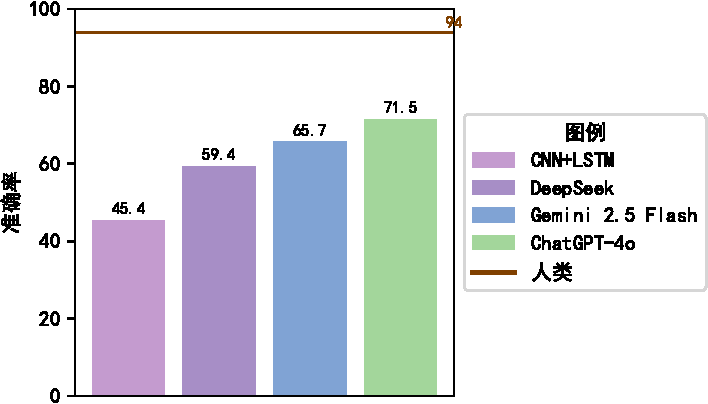
\includegraphics[scale=0.8]{figures/dataset-experiment-crop.pdf}
\caption{不同方法在POVQAD上回答问题的准确率}
\label{fig:dataset-comparison}
\end{figure}
\section{本章小结}
本章聚焦CLEVR数据集的场景完全可见、不要求模型使用外部背景知识进行推理等方面的缺陷,构建一个新的数据集POVQAD,以满足
本文对部分可见积木世界场景下空间推理问答的研究需要。

本章为后续神经符号VQA框架在部分可见积木世界场景下的空间推理问答的实验与分析奠定了坚实的数据基础。

\chapter{神经符号VQA框架的架构设计与实现}
本章将详细介绍神经符号框架的架构设计与实现,包括流水线总体架构、视觉场景理解、语义解析、迭代反馈和规则修正、规则蒸馏、ASP推理等模块的设计和实现。
框架的设计目标如下:
\begin{enumerate}[label=(\arabic*),itemsep=0pt,parsep=0pt]
\item 借鉴已有的神经符号框架的设计思路,添加、修改部分模块,提升框架对ASP规则的自动拓展能力,进而进一步增强VQA系统回答部分可见问题的准确率。
\item 使用Dspy来完成对LLM的提示、优化,以降低神经符号方法的开发难度。
\end{enumerate}
\section{框架总体架构}
框架的总体架构如图\ref{fig:pipeline}所示。其中,LLM在整个框架中的作用有以下两点:
\begin{enumerate}[label=(\arabic*),itemsep=0pt,parsep=0pt]
    \item 在语义解析模块中,LLM对自然语言问题进行语义解析,将问题以ASP的形式表示出来,以便后续
输入到迭代反馈模块中进行修正。
    \item 在迭代反馈模块中,LLM对ASP表示进行多次迭代优化,其中包括解析错误、基础化错误等。每一轮迭代都将
根据上一轮的错误信息进行针对性的修正。
    \item 在规则蒸馏中,LLM结合ASP知识库中的先验知识,对迭代反馈修正后ASP规则进行进一步补全,为Clingo求解器
推理提供更全面的知识。
    \item 在求解结果翻译中,LLM 将 Clingo 求解器输出的 ASP 表达结果翻译为自然语言形式,以回答提出的问题。
\end{enumerate}
\begin{figure}
    \centering
    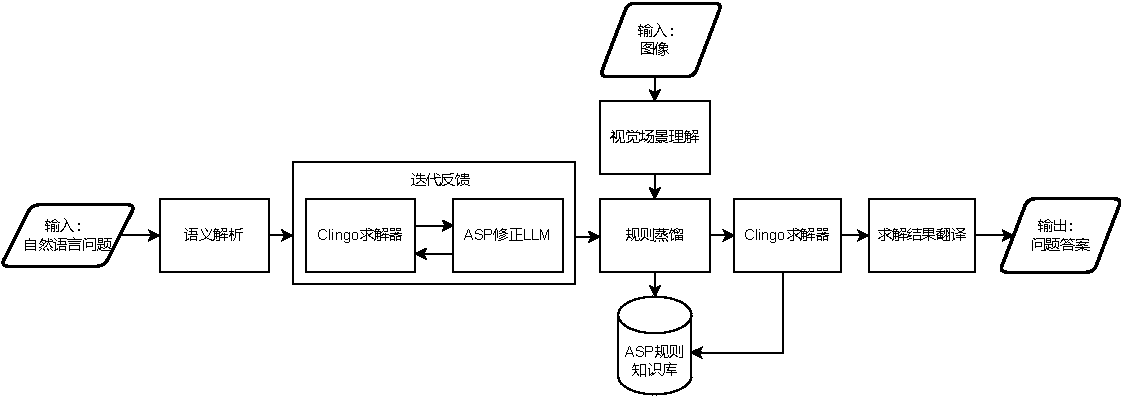
\includegraphics[width=\textwidth]{figures/pipeline-crop.pdf}
    \caption{面向空间推理领域的神经符号框架示意图}
    \label{fig:pipeline}
\end{figure}
本文在语义解析模块和迭代反馈模块中,分别采用不同的LLM,各自进行微调,以更好地满足不同任务的需求。
\section{视觉场景理解}\label{visual-recognition}
视觉场景理解是本文所设计流水线中的核心模块,其目标是从输入图像中提取结构化信息,包括物体的属性(如形状、颜色、大小等)、位置信息以及物体间的空间关系。这些信息将被进一步转换为ASP的形式,为后续基于逻辑推理的语义解析与问答模块提供形式化的知识基础。

本章主要围绕以下四个方面展开详细阐述:目标检测、空间位置提取、空间关系提取以及场景图生成。最后,本文给出一个完整的视觉场景理解演示案例,并讨论在实现过程中遇到的关键技术挑战及相应解决方案。
\subsection{目标检测}
目标检测是视觉场景理解的最基本的任务,其目标是从图像中识别出所有相关物体,并标注其边界框、类别和属性。本文选择GLIP模型作为目标检测的实现工具,原因在于
其独特的语言-视觉预训练特性。基于大规模的图文对数据,GLIP进行大量预训练,能够根据自然语言描述(如“红色立方体”)直接定位图像中的对应物体。
这种能力特别适合VQA任务,使问题中的语言信息与图像内容高效对齐成为可能。

目标检测是视觉场景理解的基础任务,其任务是从输入图像中识别出所有相关物体,
并为每个物体确定其边界框、类别和相关属性。本文采用了GLIP模型作为目标检测的核心工具,其主要优势体现在:
\begin{enumerate}[label=(\arabic*),itemsep=0pt,parsep=0pt] 
\item \textbf{语言-视觉预训练能力:}GLIP在大规模图文对数据上进行预训练,能够根据自然语言描述(例如“红色立方体”)直接定位图像中的对应物体,从而实现图像内容与问题描述的高效对齐; 
\item \textbf{高效性与鲁棒性:}模型在处理多样化场景时具有较高的检测准确率,适合构造后续依赖视觉信息的场景图。 
\end{enumerate}

具体实现流程如下:
\begin{enumerate}[label=(\arabic*),itemsep=0pt] 
\item \textbf{图像预处理:}将原始图像调整至GLIP模型要求的输入分辨率(例如800$\times$1333像素),
以保证检测精度; 
\item \textbf{文本提示构造:}根据数据集构造要求,设计一组覆盖目标类别及属性的自然语言提示。
本文选取的提示短语包括描述物体大小(如“大物体”、“小物体”)以及颜色与形状组合(如“红色立方体”、“蓝色球体”、“绿色圆柱体”等); 
\item \textbf{目标检测与属性解析:}将图像和文本提示输入GLIP,获得每个检测物体的边界框和类别标签。随后对类别标签进行解析,将复合描述(如“红色立方体”)拆解为单独属性(color=red, shape=cube)。同时,通过计算边界框面积($(x_2 - x_1)\times(y_2 - y_1)$),结合预设阈值进一步推断物体的大小属性。 
\end{enumerate}

例如,对于一张包含“红色立方体”和“蓝色球体”的图像,GLIP可能检测出如下信息: 
\begin{enumerate}[itemsep=0pt,parsep=0pt] 
\item 物体1:类别为“红色立方体”,边界框坐标为$(x_1, y_1, x_2, y_2)$; 
\item 物体2:类别为“蓝色球体”,边界框坐标为$(x_3, y_3, x_4, y_4)$。 
\end{enumerate}
\subsection{空间位置提取}
在完成目标检测后,接下来的任务是为每个物体确定其精确的空间位置,这对于后续空间关系的推理至关重要。
本文采用以下两种方式提取物体位置信息:
\begin{enumerate}
\item \textbf{二维中心点计算}:利用目标检测得到的边界框信息,计算物体在图像平面内的中心点坐标。公式如下:
$$x_c = \frac{x_1+x_2}{2}, y_c = \frac{y_1 + y_2}{2}$$
该中心点坐标用于描述物体在二维图像中的位置;
\item \textbf{三维位置信息获取}:若图像同时包含深度信息(例如通过Blender渲染生成的场景),则可直接从深度图中提取物体的z值,从而获得物体在三维空间中的位置,
表示为$(x, y, z)$。
\end{enumerate}

提取出的位置信息将以ASP事实的形式进行存储,例如:position(obj1, x1c, y1c, z1) 表示物体1的中心点位置。
\subsection{空间关系提取}
空间关系的提取是实现复杂场景理解与多步逻辑推理的关键。本文从以下几个角度对空间关系进行提取:
\begin{enumerate}[label=(\arabic*),itemsep=0.5em] 
\item \textbf{二维空间关系:}基于物体的中心点坐标计算物体之间的相对位置。例如: 
    \begin{itemize}[leftmargin=2em] 
        \item 若物体A的$x_c$小于物体B的$x_c$,则判定A位于B的左侧,表示为\texttt{left(objA, objB)}; 
        \item 类似地,通过比较$y_c$坐标可判定上下关系(例如,若物体A的$y_c$小于B,则A在B之上,记作\texttt{above(objA, objB)})。 
    \end{itemize} 
\item \textbf{三维空间关系:}利用深度信息,对物体间的前后关系进行判断。
例如,若物体A的z值小于物体B的z值,则判定A位于B的前面,记作\texttt{in\_front\_of(objA, objB)}。 
\item \textbf{遮挡关系:}结合边界框重叠情况与深度信息进行判断。如果两个物体边界框存在重叠且A的深度值明显小于B,
则可以认为A遮挡B,记作\texttt{occludes(objA, objB)}。 
\end{enumerate}
所有提取到的空间关系均转换为ASP事实,如:
left(obj1, obj2) 表示物体1在物体2的左边,in\_front\_of(obj1, obj2) 表示物体1在物体2的前面;
occludes(obj1, obj2) 表示物体1遮挡了物体2。
\subsection{场景图生成}
场景图是将目标检测、空间位置与空间关系综合融合成的统一结构化表示,其主要构成如下: 
\begin{enumerate}[label=(\arabic*),itemsep=0.5em] 
    \item \textbf{节点表示:}每个节点对应图像中的一个物体,并附有相应的属性(如color, shape, size, material)以及位置信息; 
    \item \textbf{边的构建:}节点之间的边用于表示物体间的空间关系,如left\_of、in\_front\_of等。 
\end{enumerate}

在构建过程中,首先为每个检测到的物体创建一个节点,并记录其属性及位置;
随后,依据前述空间关系,将相应的有向边添加到图中。
最终,整个场景图将被转化为ASP事实,以支持后续符号推理任务。
\subsection{实现细节与实例}
为便于说明,下面给出一个具体示例。假设输入图像包含如下场景: 
\begin{enumerate}[label=(\arabic*),itemsep=0.5em] 
    \item 一个红色大立方体位于图像左侧; 
    \item 一个蓝色小球体位于图像右侧,且位于红色立方体的前方。 
\end{enumerate}

经过GLIP目标检测,得到如下检测结果: 
\begin{itemize}[leftmargin=2em] 
    \item 物体1:类别为“红色立方体”,边界框为(50, 100, 150, 200); 
    \item 物体2:类别为“蓝色球体”,边界框为(250, 50, 350, 150)。 
\end{itemize}

进一步计算得到: 
\begin{itemize}[leftmargin=2em] 
    \item 物体1的中心点坐标为$(100,150)$; 
    \item 物体2的中心点坐标为$(300,100)$。 
\end{itemize}

假设深度信息显示:物体1的z值为50,物体2的z值为75,则可提取以下空间关系: 
\begin{itemize}[leftmargin=2em] 
    \item \texttt{left\_of(obj1, obj2)}(因为100 $<$ 300); 
    \item \texttt{above(obj2, obj1)}(因为100 $<$ 150); 
    \item \texttt{in\_front\_of(obj2, obj1)}(因为75 $>$ 50,在三维空间中深度值较大的物体更靠后,需根据具体定义调整)。 
\end{itemize}

最终生成的ASP事实示例如下: 
\begin{lstlisting}[language=Prolog] 
color(obj1, red). 
shape(obj1, cube). 
size(obj1, large). 
position(obj1, 100, 150, 50).

color(obj2, blue). 
shape(obj2, sphere). 
size(obj2, small). 
position(obj2, 300, 100, 75).

left_of(obj1, obj2). 
above(obj2, obj1). 
in_front_of(obj2, obj1). 
\end{lstlisting}
\subsection{技术挑战与解决方案}
在实际实现过程中,本模块面临如下关键技术挑战,并提出相应解决方案: 
\begin{enumerate}[label=(\arabic*),itemsep=0.5em] 
    \item \textbf{检测准确性}:GLIP 在处理物体密集或遮挡严重的场景时,可能存在误检问题。为此,本文引入非极大值抑制(NMS)以及深度信息辅助过滤,提高检测精度; 
    \item \textbf{空间关系鲁棒性}:二维关系受视角影响较大,为增强鲁棒性,本文在有深度信息的条件下优先采用三维关系,并结合几何约束(例如边界框重叠)进行补充; 
    \item \textbf{计算效率}:面对大规模图像数据,为保证系统实时性,本文通过批量处理图像以及优化提示设计,有效降低了GLIP的推理延时。
\end{enumerate}
\subsection{小结}
本节详细介绍了基于GLIP的视觉场景理解模块的整体架构与实现细节。
通过对目标检测、空间位置与空间关系的综合提取,最终构建了能够转化为ASP事实的场景图,
为后续语义解析和逻辑推理提供了坚实的数据基础。
下一节将介绍如何利用LLM将自然语言问题转化为ASP查询,实现语义解析与神经符号推理的无缝衔接。
\section{语义解析}
语义解析的主要任务是使用 LLM 将自然语言问题转换为 ASP 表达形式,获得ASP规则,以便与视觉场景理解提取的场景事实结合进行逻辑推理。

直观上,LLM可能很难直接解决复杂的推理问题。然而,LLM已经在理解文本输入并将其转化为形式化程序方面取得了巨大成功,
例如程序代码\cite{gao2023pal}和数学方程\cite{he2023solving}。为了让LLM更准确地生成ASP编码,本文在此对通用LLM进行针对性微调。
\subsection{微调数据集模板设计}
现有的通用代码生成数据集可能无法充分覆盖ASP中普遍存在的特定结构和模式,而对LLM针对特定任务进行微调,面向特定领域的数据集必不可少。
因此,对LLM针对ASP编码任务进行微调的核心是:创建一个涵盖多种ASP问题类别的微调数据集。
通过创建一个有针对性的数据集,模型可以更有效地学习这些特定的细微差别。

本文以下对常见的ASP编程任务进行分析,确定了以下9种ASP编码的基本情形,分别为其设计模板,用于后续构建微调数据集。
\subsubsection{猜测赋值}
猜测赋值是ASP编码中的经典情形。具体而言,猜测赋值指的是将某一给定集合中的所有元素赋予一个从固定集合中选出的唯一标签。
在ASP中,通常使用析取来表示“猜测”。以下是猜测赋值的一个示例。
\begin{lstlisting}
模板:为以下问题编写一个 ASP 程序。在给定的一组标签中,为元素集准确分配一个标签。元素集由谓词 [PREDICATE] 表示。标签为 [LABEL]+。
提示:为以下问题编写一个 ASP 程序。在给定的一组标签中,为元素集准确分配一个标签。元素集由谓词 city 表示。标签为 moscow、rome、dubai。
编码:assign(X,"moscow") |assign(X,"rome") | assign(X,"dubai") :- city(X).
\end{lstlisting}
\subsubsection{表达约束}
表达约束表示必须满足的条件。在ASP中,这通常通过(经典/强)约束来实现,有时会使用辅助规则。以下是表达约束的一个示例。
\begin{lstlisting}
模板:为以下问题编写一个 ASP 程序。防止值为 [VALUE] 的谓词 [PREDICATE] 带有标签 [LABEL]。
提示:为以下问题编写一个 ASP 程序。防止值为 11 的谓词 car 带有标签“red”。
编码: :- assign(11,"red").
\end{lstlisting}
\subsubsection{生成组合}
生成组合指创建来自两个不同集合的所有可能的元素组合(笛卡尔积)。在ASP中,可以通过简单的规则完成。以下是生成组合的一个示例。
\begin{lstlisting}
模板:为以下问题编写一个 ASP 程序。从两个集合生成所有元素组合。这两个集合分别由谓词 [PREDICATE_1] 和 [PREDICATE_2] 表示。
提示:为以下问题编写一个 ASP 程序。从两个集合生成所有元素组合。这两个集合分别由谓词 city 和 airport 表示。
编码: combination(X,Y) :- city(X), airport(Y).
\end{lstlisting}
\subsubsection{连接}
连接指的是基于特定匹配标准将来自两个不同集合的元素关联起来。在ASP中,通常通过在规则体中具有共享变量的文字来定义。以下是连接的一个示例。
\begin{lstlisting}
模板:为以下问题编写一个 ASP 程序。假设谓词 [PREDICATE_1] 具有字段 [LABEL]+,谓词 [PREDICATE_2] 具有字段 [LABEL]+。定义一个谓词 [PREDICATE_1]_[PREDICATE_2],将每个 [PREDICATE_1] 与 [PREDICATE_2] 的 [LABEL] 关联。
提示:为以下问题编写一个 ASP 程序。假设谓词“owner”具有字段“ID”、“surname”、“name”、“restaurantID”,谓词“restaurant”具有字段“ID”、“description”。定义一个谓词“owner_restaurant”,将每个所有者与餐厅的描述关联。
编码:owner_restaurant(X,Z) :-owner(X,_,_,Y),restaurant(Y,Z).
\end{lstlisting}
\subsubsection{传递闭包}
传递闭包用于定义超出直接连接的关系,捕获由一系列关系形成的间接关系。在ASP中,通常需要多个规则,通常涉及递归。以下是传递闭包的一个示例。
在该示例中,编码使用了两条规则:一条用于定义直接关系,另一条(依赖递归)用于捕捉间接关系。
\begin{lstlisting}
模板:为以下问题编写一个 ASP 程序。将谓词 [PREDICATE_1] 定义为谓词 [PREDICATE_2] 的传递闭包。
提示:为以下问题编写一个 ASP 程序。将谓词“arrivals”定义为谓词“flight”的传递闭包。
编码:arrivals(X,Y) :- flight(X,Y).
arrivals(X,Y) :- flight(X,Z),arrivals(Z,Y).
\end{lstlisting}
\subsubsection{表达偏好}
表达偏好用于定义对一组可接受解决方案的偏好,通常用于解决优化问题。在ASP中,通常通过编码带有弱约束的程序来完成。以下是表达偏好的一个示例。
\begin{lstlisting}
模板:为以下问题编写一个 ASP 程序。我希望值为 18 的谓词 [PREDICATE] 与 [LABEL] 不相关联。如果发生这种情况,则在级别 [LEVEL] 上花费 [COST]。
提示:为以下问题编写一个 ASP 程序。我希望值为 18 的谓词 house 与“flat”不相关联。如果发生这种情况,则在级别 2 上花费 2。
编码::∼assign(18,"flat").
\end{lstlisting}
\subsubsection{按值过滤}
在编写 ASP(回答集程序)时,通常需要根据特定的需求对某些谓词的外延进行过滤。按值过滤的过滤标准是:选取某个谓词外延中与特定值匹配的部分。
以下是按值过滤的一个示例。
\begin{lstlisting}
模板:为以下问题编写一个 ASP 程序。选择与标签为 [LABEL] 的谓词 [PREDICATE] 相关联的所有值。
提示:为以下问题编写一个 ASP 程序。选择与标签为“purple”的谓词 color 相关联的所有值。
编码:select(X) :- color(X,"purple").
\end{lstlisting}
\subsubsection{负过滤}
负过滤的过滤标准是:排除与给定条件匹配的谓词扩展部分。具体而言,可以是两个谓词外延之间的差集(减法运算),也可以是复合条件的否定。
以下是负过滤的一个示例。
\begin{lstlisting}
模板:为以下问题编写一个 ASP 程序。选择与谓词 [PREDICATE_1] 关联但与谓词 [PREDICATE_2] 和标签 [LABEL] 不关联的所有值。
提示:为以下问题编写一个 ASP 程序。选择与谓词 vehicle 关联但与谓词 moto 和标签“kawasaki”不关联的所有值。
编码:select(X) :- vehicle(X),
not moto(X,"kawasaki")。
\end{lstlisting}
\subsubsection{按数值比较过滤}
按数值比较过滤的过滤标准是:根据项之间比较的结果,对表格中部分内容进行过滤。
以下是按数值比较过滤的一个示例。
\begin{lstlisting}
模板:为以下问题编写一个 ASP 程序。选择与谓词 [PREDICATE] 关联且值大于或等于 [VALUE] 的所有值。
提示:为以下问题编写一个 ASP 程序。选择与谓词 size 关联且值大于或等于 5 的所有值。
编码:select(X) :- size(X,C), C>=5。
\end{lstlisting}

通过明确定义不同ASP任务的模板,可以系统地生成数据,确保覆盖基本的ASP概念,并允许在需要时系统地扩展数据集。
使用模板可以程序化地生成庞大且多样化的数据集,这比手动创建大型数据集更有效且更可控。
\subsection{微调数据集生成}
本文将所需生成的微调数据集记为$D$,包含自然语言描述的ASP任务及其对应的标准ASP程序片段,二者构成一个二元组。
数据集的结构基于一个模板集$T = (P, A)$,其中$P$是自然语言描述的集合,$A$是ASP程序的集合 。
T进一步划分为${TC_1, TC_2,..., TC_k}$,每个$TC_i$代表一种特定的任务类型,例如猜测赋值、表达约束、生成组合、连接、传递闭包、表达偏好和过滤。

对于每种任务类型,通过实例化包含谓词、标签和值的占位符来生成模板的变体,这些谓词、标签和值来自预定义的集合 。由此产生的完整数据集$D$大约包含3.7万个元组 。
数据集中不同任务类型元组的数量占比取决于每种任务所需的ASP代码的句法复杂性,具体各类型占比见表\ref{tab:task-portion}。
对应ASP程序中变异性较大的任务(例如规则中谓词数量、原子元的元数(arity)、以及实例的具体化情况)在训练过程中需要更多数据。
最终,数据集被分成训练集(80\%)和验证集(20\%),并且在两个集合中都保持了每种问题类型的比例 。

\begin{table}[ht]
\centering
\begin{tabular}{lrr}
\toprule
\textbf{ASP任务类型} & \textbf{元组数量} & \textbf{占比(\%)} \\
\midrule
赋值          & 10000 & 27.0 \\
约束          &   5000 & 13.5 \\
组合         &   1000 & 2.7 \\
连接                &   9000 & 24.3 \\
闭包  &   1000 & 2.7 \\
偏好          &   4000 & 10.8 \\
按值过滤     &   1000 & 2.7 \\
负过滤  &   1000 & 2.7 \\
按数值比较过滤   &   5000 & 13.5 \\
\midrule
\textbf{Total}      & 37000 & 100 \\
\bottomrule
\end{tabular}
\caption{微调数据集中的各类型ASP任务数量及其占比}
\label{tab:task-portion}
\end{table}

\subsection{模型选择与微调}
目前,工业界已推出众多LLM,这些LLM在架构、参数量和训练数据集等方面各有不同。本文聚焦于一些开源LLM,这些开源的LLM也代表了当前LLM领域的最新研究成果。
选用的LLM如下:
\begin{enumerate}[itemsep=0pt,parsep=0pt]
\item \textbf{ChatGPT-4o}:由OpenAI于2024年发布的多语言、多模态LLM。
\item \textbf{DeepSeek-Coder}:由深度求索公司发布的开源代码大模型系列,专注于代码生成、补全、调试及跨语言转换等编程任务。
\item \textbf{LLama3}:LLaMa 模型的增强版,在推理、代码生成和遵循指令等任务中有显著提升。
\end{enumerate}
表\ref{tab:llm-comparison}简要对比了所选LLM的参数规模、架构和训练数据来源。
从中可以识别出两个模型规模群体:一个是大型模型组(参数量 ≥ 700 亿),另一个是小型模型组(参数量 < 700 亿);其中DeepSeek-Coder 1.3B是本次实验中体积最小的模型。

\begin{table}[ht]
    \centering
    \begin{tabular}{lccc}
        \toprule
        \textbf{模型} & \textbf{参数量} & \textbf{架构} & \textbf{训练数据源} \\
        \midrule
        ChatGPT-4o    & 200B      & 多模态统一网络           & 网络数据         \\
        DeepSeek-Coder       & 1.3B--33B      & MoE + MLA            & 网络数据    \\
        LLaMa3         & 8B--70B   & 纯解码器 + 分组查询注意力机制   & 网络数据         \\
        \bottomrule
    \end{tabular}
    \caption{LLM对比详细信息,其中参数量以十亿(B)为单位。}
    \label{tab:llm-comparison}
\end{table}

在众多模型中,本文选用DeepSeek-Coder 1.3B作为微调模型。选择其的主要原因是,其体积是当前主流可用模型中最小的,
可以预见未经过训练的原始DeepSeek-Coder 1.3B模型在解答问题的正确率等评估指标上的表现相对较差,从而可以更直观地评估微调的效果。

数据集构建完成后,采用DSPy对LLM进行微调,使用上述的微调数据集样例的输入输出格式来DSPy程序定义输入输出签名,
选择本地的DeepSeek-Coder 1.3B进行接口配置。评估指标使用ASP程序执行率。

构建DSPy程序的过程中,使用DSPy的Template组件定义提示模板,
指导LLM如何生成指定格式的ASP程序。也使用了Example组件,用于构建优化过程中使用的示例数据,
封装输入和输出的对应关系,以帮助LLM进行学习。与传统的LLM开发流程相比,DSPy框架自动化管理了提示模板和
示例数据的构建过程,有效降低了手动调试和反复迭代的复杂度,从而大幅简化了整个LLM相关的开发流程,
显著提高了开发效率和模型优化的便捷性。此外,为了提高计算效率,在微调过程中采用了QLoRA(Quantization-aware Low-Rank Adaptation,量化感知低秩适应) 。
QLoRA通过量化模型权重并使用低秩适配器进行有效的参数更新,从而减少了内存占用和计算成本,使得在有限的资源上进行微调成为可能 。
\subsection{模型评估}
本文使用ASP求解器Clingo评估LLM生成的ASP程序的正确性。对于一个程序$P$,Clingo用于计算该程序的答案集。
进而该过程可以等价于:定义一个函数$f(P) = AS(P)$,其中$AS(P)$表示程序P的所有回答集(可能为空)。

LLM根据提示$x$生成的ASP程序,记为$y ~ P_L(|x)$。与$x$对应的能够真实表示问题的标准ASP程序,记为$y^*$。按照以下步骤来进行验证:
首先基于$x$构建一个表示具体实例的事实集$F_{y^*}$。接着,构造两个完整的ASP程序:
\begin{enumerate}[itemsep=0pt,parsep=0pt]
\item $P = y \cup F_{y^*}$:由模型生成程序与事实集合成的程序。
\item $P^* = y^* \cup F_{y^*}$:由标准程序与事实集合成的程序。
\end{enumerate}

此后,执行以下评估步骤:
\begin{enumerate}
\item 语法检查:调用Clingo运行程序$P$,若未发生解析错误,则认为模型生成的程序 $y$ 在语法上是正确的,则判定为语法命中。否则,则判定为不命中。
\item 语义检查:分别用 Clingo 计算$f(P)$与$f(P^*)$,分别得到各自的答案集$AS(P)$与$AS(P^*)$。若$AS(P)$与$AS(P^*)$完全匹配,则判定为语义命中。
否则,则判定为不命中。
\end{enumerate}

评估指标选用语法准确率和语义准确率。
\subsection{实验与结果分析}
为检测语义解析模块的性能,本文使用上一小节构造的数据集进行实验。考核指标选取上一节定义的语法命中率和语义命中率。
将未经过训练的LLM与本文经微调后的DeepSeek-Coder 1.3B模型进行对比。在实验过程中,对实验重复进行5次,以
降低LLM采样过程的随机性带来的影响。

实验结果如表\ref{fig:overall_syntactics_semantics}及图\ref{fig:syntactics_and_semantics}所示。
由实验结果可以看出,语法正确并不能保证语义正确,例如,LLaMa3 8B实现了58\%的语法正确率,但是语义正确率明显偏低。
总的来看,没有任何模型能够做到全方面正确,轻量级模型的表现普遍较差。
此外,ChatGPT-4o实现了高达100\%的语法正确率。本文的经微调后的DeepSeek-Coder 1.3B模型在所有模型中的语义准确率最高。
根据实验结果,也能够看出,当生成的ASP程序在语法上正确时,其语义正确的可能性也会更大。

所有模型在每种类型的任务上的语法正确率和语义正确率的对比见表\ref{tab:semantics_comparison}。与其它LLM相比,微调后模型仅在
生成组合任务中由于语法错误而导致表现不佳。
\begin{figure}
    \centering
    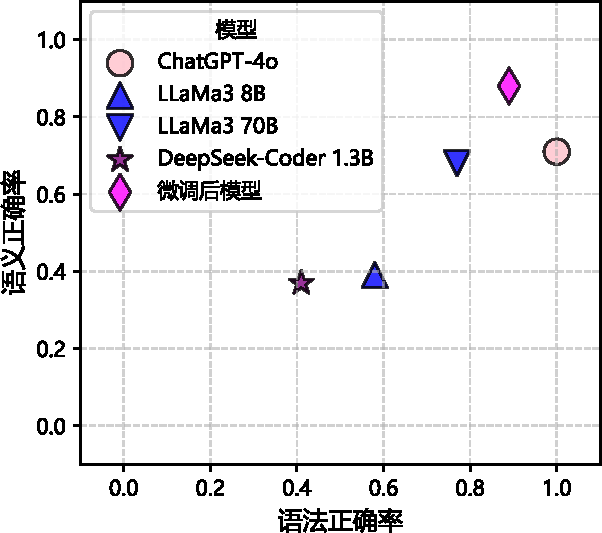
\includegraphics{figures/synatics_and_semantics-crop.pdf}
    \caption{各模型的语法正确率及语义正确率}
    \label{fig:syntactics_and_semantics}
\end{figure}
\begin{table}
    \centering
    \begin{tabular}{lcc}
        \toprule
        \textbf{模型} & \textbf{语法正确率} & \textbf{语义正确率} \\
        \midrule
        ChatGPT-4o & 1 & 0.71 \\
        Llama3 8B & 0.58 & 0.39 \\
        Llama3 70B & 0.77 & 0.68 \\
        DeepSeek-Coder 1.3B & 0.41 & 0.37 \\
        \midrule
        微调后模型 & 0.89 & 0.88 \\
        \bottomrule
    \end{tabular}
    \caption{各模型在语法和语义方面的对比分析}
    \label{fig:overall_syntactics_semantics}
\end{table}
\begin{table}[h]
    \centering
    \renewcommand{\arraystretch}{1.2}
    \setlength{\tabcolsep}{5pt}
    \resizebox{\textwidth}{!}{
    \begin{tabular}{lcccccccccccccccccc}
        \toprule
        \multirow{2}{*}{模型} & \multicolumn{2}{c}{猜测赋值} & \multicolumn{2}{c}{表达约束} & \multicolumn{2}{c}{生成组合} & \multicolumn{2}{c}{连接} & \multicolumn{2}{c}{传递闭包} & \multicolumn{2}{c}{表达偏好} & \multicolumn{2}{c}{按值过滤} & \multicolumn{2}{c}{负过滤}& \multicolumn{2}{c}{按数值比较过滤}  \\
        \cmidrule(lr){2-3} \cmidrule(lr){4-5} \cmidrule(lr){6-7} \cmidrule(lr){8-9} \cmidrule(lr){10-11} \cmidrule(lr){12-13} \cmidrule(lr){14-15} \cmidrule(lr){16-17} \cmidrule(lr){18-19}
        & \textit{语法} & \textit{语义} & \textit{语法} & \textit{语义} & \textit{语法} & \textit{语义} & \textit{语法} & \textit{语义} & \textit{语法} & \textit{语义} & \textit{语法} & \textit{语义} & \textit{语法} & \textit{语义} & \textit{语法} & \textit{语义} & \textit{语法} & \textit{语义}\\
        \midrule
        ChatGPT-4o & 1 & 0.8 & 1 & 1 & 1 & 1 & 1 & 1 & 1 & 1 & 1 & 0 & 1 & 0 & 1 & 0 & 1 & 1\\
        LLama3 8B & 0.6 & 0.4 & 0.5 & 0.5 & 0 & 0 & 0 & 0 & 1 & 0.7 & 0.3 & 0.3 & 0.4 & 0.4 & 0.2 & 0 & 0 & 0 \\
        LLama3 70B & 0.8 & 0.8 & 0.4 & 0.3 & 1 & 1 & 0.7 & 0.7 & 0.9 & 0.7 & 0 & 0 & 0.8 & 0.8 & 0.8 & 0.7 & 1 & 1\\
        DeepSeek-Coder 1.3B & 0.6 & 0.4 & 0.7 & 0.2 & 0 & 0 & 1 & 0.8 & 1 & 1 & 0 & 0 & 0.6 & 0.1 & 0.2 & 0 & 1 & 1 \\
        \midrule
        \textbf{微调后模型} & 1 & 0.9 & 1 & 1 & 0 & 0 & 1 & 1 & 1 & 1 & 1 & 1 & 1 & 1 & 0.8 & 0.7 & 1 & 1 \\
        \bottomrule
    \end{tabular}
    }
    \caption{不同模型在各问题类型上的语法正确率和语义正确率的对比}
    \label{tab:semantics_comparison}
\end{table}

为了进一步评估微调后模型的鲁棒性,本文将其与其它模型在拓展的测试集上进行了比较,其中的提示在谓词和标签方面进行了些许改动。
具体实验结果见表\ref{tab:robust1}。
结果显示,尽管微调后模型偶尔存在语法缺陷,但其生成ASP程序更加可靠,性能比排名第二的模型高出8\%。
此外不难看出,只要语法正确,问题的语义也能得到满足。

\begin{table}[h]
\centering
\begin{tabular}{lcc}
\toprule
\textbf{Model} & \textbf{Syntactic} & \textbf{Semantic} \\
\midrule
ChatGPT-4o     & 1   & 0.67 \\
DeepSeek-Coder 1.3B         & 1     & 0.57 \\
LLama3 8B      & 1     & 0.85 \\
LLama3 70B    & 1     & 0.69 \\
\midrule
\textbf{微调后模型}  & 0.93 & 0.93 \\
\bottomrule
\end{tabular}
\caption{使用拓展的测试集进行进一步比较的结果}
\label{tab:robust1}
\end{table}
\section{迭代反馈与规则修正}\label{rule-fix}
迭代反馈模块是整个神经符号集成管道的核心部分,其主要功能在于对语义解析模块生成的ASP程序进行检查,如果有错误,则使用LLM对其进行修正。
\subsection{流程概述}
整个迭代反馈与规则修正的大致流程如下:
\begin{enumerate}[itemsep=0pt,parsep=0pt]
\item 使用Clingo求解器对语义解析模块生成的ASP程序尝试执行。
\item 如果执行成功,没有提示错误,则无需进行进一步修正,直接将ASP程序流转到框架的下一模块。
\item 如果执行失败,则将错误的ASP程序和Clingo求解器提示的错误信息,一起输入LLM,由LLM尝试进行修正。
\item 将修正后的ASP程序再次输入到Clingo求解器中,尝试执行。如此循环最多3次,最终输出经过优化后的ASP程序,流转到框架的下一模块。
\end{enumerate}
\subsection{错误类型与修正策略}
不同类型的错误信息对应着ASP程序中不同的问题,因此需要采用不同的修正策略。本文设计了多套提示模板,用以指导LLM针对性地进行程序修正。
\begin{enumerate}[itemsep=0pt,parsep=0pt]
\item \textbf{语法错误}:这类错误通常发生在程序违反了ASP的语法规则时。错误信息会指出文件、行号、列号以及意料之外的符号 。例如,遗漏句点、括号不匹配或使用了Clingo版本不支持的语法都可能导致语法错误 。
以下是该错误的一个提示词模板:
\begin{lstlisting}
任务描述:请根据提供的 ASP 程序和 Clingo 错误信息,对程序进行修正。

错误类型:语法错误 (Syntax Error) - 规则或事实缺少句号。

错误程序:
node(a).
node(b) % <- 错误:这里缺少句号
edge(a, b).

path(X, Y) :- edge(X, Y).
path(X, Z) :- edge(X, Y), path(Y, Z).

Clingo错误信息:
<stdin>:3:1: error: syntax error, unexpected IDENTIFIER, expecting '.' or ':
  node(b) % <- 错误:这里缺少句号

修正后程序:
node(a).
node(b). % <- 修正:添加句号
edge(a, b).

path(X, Y) :- edge(X, Y).
path(X, Z) :- edge(X, Y), path(Y, Z).
\end{lstlisting}
\item \textbf{谓词未定义}:这通常是一个警告,表示某个谓词在规则体中被使用,但从未在任何规则的头部定义过 。
程序执行不会因此停止,但可能暗示着逻辑错误 。以下是该错误的一个提示词模板:
\begin{lstlisting}
任务描述:请根据提供的 ASP 程序和 Clingo 错误信息,对程序进行修正。

错误类型:未定义的谓词(Undefined Predicate)

错误程序:
p(a) :- q(a).

Clingo错误信息:
error: in rule at line 1: undefined predicate: q/1

修正后程序:
q(a).
p(a) :- q(a).
\end{lstlisting}
\item \textbf{循环负依赖}:循环负依赖发生在程序的依赖图中存在负循环,即一个谓词通过一系列规则负依赖于自身。
负循环可能导致程序没有解答集。​此外在某些情况下,可能导致多个解答集的产生,增加了解释的复杂性。以下是该错误的一个提示词模板:
\begin{lstlisting}
任务描述:请根据提供的 ASP 程序和 Clingo 错误信息,对程序进行修正。

错误类型:​递归中的负循环(Negative Cycle in Recursion)​

错误程序:
p(X) :- not q(X).
q(X) :- not p(X).

Clingo错误信息:
error: in rule at line 2: cyclic dependency: p/1 -> q/1 -> p/1

修正后程序:
p(X) :- r(X), not q(X).
q(X) :- s(X), not p(X).
\end{lstlisting}
\item \textbf{重复的规则或者事实}:这类错误往往是由于人为输入错误或多个ASP程序进行合并时,没有去重导致。以下是该错误的一个提示词模板:
\begin{lstlisting}
任务描述:请根据提供的 ASP 程序和 Clingo 错误信息,对程序进行修正。

错误类型:​重复的规则或事实(Duplicate Rules or Facts)​

错误程序:
p(a).
p(a).

Clingo错误信息:
warning: fact at line 2 is a duplicate of fact at line 1

修正后程序:
p(a).
\end{lstlisting}
\item \textbf{约束条件恒为假}:在ASP中,约束条件的作用是排除使Body为真的解答集。
当约束条件的Body部分恒为真时,该约束条件始终排除所有可能的解答集。出现这一错误时,由于所有可能的解答集都被排除,程序将没有解答集,即程序不一致。
\begin{lstlisting}
任务描述:请根据提供的 ASP 程序和 Clingo 错误信息,对程序进行修正。

错误类型:​约束条件总为假(Constraint Always False)

错误程序:
:- p(X), not p(X).

Clingo错误信息:
warning: constraint at line 1 is always false

修正后程序:
:- p(X), not q(X).
\end{lstlisting}
\item \textbf{不安全变量}:当一个变量出现在规则的头部,但没有在规则体的任何肯定字面量中出现时,就会发生这种错误 。这可能会导致产生无限的稳定模型 。Clingo会报告出错的规则以及不安全的变量名 。以下是该错误的一个提示词模板:
\begin{lstlisting}
任务描述:请根据提供的 ASP 程序和 Clingo 错误信息,对程序进行修正。

错误类型:基础化错误 (Grounding Error) - 规则中存在不安全变量。

错误程序:
reachable(X) :- edge(Y, X). % <- 错误:变量 Y 是不安全的,因为它没有在规则头或任何正文字面量中安全出现

Clingo错误信息:
<stdin>:5:20-21: error: variable Y is unsafe
  reachable(X) :- edge(Y, X). % <- 错误:变量 Y 是不安全的...

修正后程序:
reachable(X) :- edge(Y, X), node(Y). % <- 修正:添加 node(Y) 来约束 Y 的范围
\end{lstlisting}
\item \textbf{不一致的事实和规则}:如果程序中定义的事实和规则之间存在矛盾,会导致出现逻辑错误。以下是该错误的一个提示词模板:
\begin{lstlisting}
任务描述:请根据提供的 ASP 程序和 Clingo 错误信息,对程序进行修正。

错误类型:逻辑错误 (Logical Error) - 程序包含直接冲突的规则或事实,导致没有稳定模型。

错误程序:
light_on. % 灯是开着的

:- light_on. % 约束:灯不能是开着的

Clingo 错误信息:
Reading from <stdin>
Solving...
UNSATISFIABLE

Models       : 0
Calls        : 1
Time         : 0.000s (Solving: 0.00s 1st Model: 0.00s Unsat: 0.00s)
CPU Time     : 0.000s

修正后程序 (根据意图选择修正): (修正方法取决于真实意图。这里假设约束是错误的)
light_on. % 灯是开着的

% :- light_on. % <- 修正:注释掉或删除冲突的约束
(或者,如果事实是错误的)
% light_on. % <- 修正:注释掉或删除冲突的事实

:- light_on. % 约束:灯不能是开着的
\end{lstlisting}
\end{enumerate}
每一轮反馈过程中,LLM都将结合Clingo返回的错误信息和预定义的提示模板进行针对性修正,
从而使生成的ASP程序在下一轮执行中更趋于正确和可执行。

\subsection{构建微调数据集并进行微调}
本文使用上述针对各类ASP程序错误类型而设计的提示模板,生成微调数据集。数据集中每条样例是一个输入-输出对,
其中输入包括任务描述、错误程序、Clingo错误信息,输出是修正后的ASP程序和错误类型。

数据集构建完成后,使用DSPy对LLM进行微调。此处选用的LLM为DeepSeek-Coder 1.3B作为微调模型。
此后,构建DSPy程序,使用上述的微调数据集样例的输入输出格式来DSPy程序定义输入输出签名,
选择本地的DeepSeek-Coder 1.3B进行接口配置。评估指标使用迭代轮数以及ASP程序执行率。

本文根据公开资料,对比了DSPy框架中提供的三种优化器的适用任务及场景,
如表\ref{tab:optimizer_comparison}所示。考虑到本文有限的标注样本和实际应用需求,最终本文选择了BootstrapFewShot优化器,实现了能够在保证优化效果的同时,
大幅提高反馈迭代的效率和系统的总体性能。

采用DSPy框架来构建LLM应用、进行微调,具有以下优势:
(1)模块化管理:DSPy将整个反馈流程拆分为若干功能模块,如ASP程序生成、错误信息解析、
提示模板更新及程序修正等。模块之间通过明确定义的接口进行通信,保证了信息的准确传递和记忆保留,
从而实现参数的自适应调整和流程优化。
(2)自动化优化:DSPy支持对LLM提示词及参数进行自动优化,极大地降低了人工调试的工作量。
在多次与LLM交互后,系统能够根据反馈动态调整提示模板,
最终得到一个较优的提示方案,以提高整体系统的修正效率和程序可执行率。
(3)日志记录与调试:为了便于调试和系统性能分析,
DSPy在整个反馈过程中对各模块的输出日志进行详细记录,包括错误信息、状态提示以及每一轮迭代的修正详情。
\begin{table}[htbp]
\centering
\caption{Dspy 框架支持的优化器比较}
\label{tab:optimizer_comparison}
\begin{tabular}{|>{\raggedright}p{4cm}|>{\raggedright}p{8cm}|>{\raggedright\arraybackslash}p{4cm}|}
\hline
\textbf{优化器名称} & \textbf{主要功能} & \textbf{适用场景} \\
\hline
BootstrapFewShot & 通过在提示中自动生成并包含优化示例来扩展签名。 & 少样本学习 \\
\hline
BootstrapFewShot-
WithRandomSearch & 在 BootstrapFewShot 的基础上,对生成的示例进行多次随机搜索,选择优化后的最佳程序。 & 少样本学习,需要更高精度 \\
\hline
MIPRO & 在每个步骤中生成指令和少量示例,使用贝叶斯优化来有效地搜索模块中的生成指令和示例空间。 & 需要复杂指令和示例优化的场景 \\
\hline
BootstrapFinetune & 将基于提示的 DSPy 程序提炼为较小语言模型的权重更新,微调底层大型语言模型以提高效率。 & 需要微调模型以提高效率的场景 \\
\hline
\end{tabular}
\end{table}
\section{规则蒸馏}
经过迭代反馈修正后的ASP编码,已经能够顺利通过Clingo求解器执行,同时在语法和语义上保证正确。然而,回答部分可见性的问题,除了问题及其对应的图像中的
知识以外,还需要利用一些已有常识作为补充。规则蒸馏的目的在于,利用LLM的知识和已有ASP知识库的知识,对迭代反馈修正后得到的
ASP编码进行补全,减轻知识工程师手动编写规则的负担,最终得到解决问题所需的足够的ASP规则,供后续Clingo求解器
使用。

本模块的技术路径如下:模块首先对输入的
当系统检测到现有的ASP规则集无法推导出问题的正确答案时,将会。
\subsection{预提示}
预提示的作用是,为LLM提供背景信息和任务说明。具体而言,预提示包括以下内容:
\begin{enumerate}[itemsep=0pt,parsep=0pt]
\item \textbf{任务介绍}:首先简要说明VQA任务的背景,告诉LLM任务的性质——给定一个问题、一个图像和它们的描述,生成相应的答案。
\item \textbf{语言语法}:介绍ASP规则的基本语法和约定。具体而言,ASP使用了一些类似于逻辑程序设计的语法,如 :-(表示规则的条件)和 not(表示否定)。
\item \textbf{场景与问题解释}:解释如何将图像场景和问题转换成ASP的表示方式。
\item \textbf{答案格式}:告诉LLM如何表示和返回问题的答案。
\item \textbf{初始ASP理论}:提供一个初始的ASP理论,它包括一些能够回答某些问题的规则,但可能不完全覆盖所有问题。
\end{enumerate}

该机制通过增量式规则扩展实现ASP知识库的动态演进:每当系统识别出现有理论无法推导正确结果时,
会触发LLM的规则生成模块,输出符合ASP语法的逻辑规则补充到ASP知识库中。
整个过程形成“问题识别-规则生成-理论扩展”的闭环优化路径。

以下\ref{distillation-prompt}为节选的部分提示词,可作为参考。
\begin{lstlisting}[label=distillation-prompt]
你的任务是对ASP知识库进行维护,通过动态更新规则确保其能够解答各类问题。ASP知识库中的现有规则已能够满足对部分问题的处理需要,
需根据输入的问题的ASP表示进行增量式规则拓展。输入提示将包含一个或多个采用ASP表示形式的问题。请严格遵守以下规则:

1. 仅输出新增的ASP规则。
2. 禁止将事实作为规则添加。不允许在规则头(head)中使用具体常量实例。
3. 将规则的泛化程度实现最大化。你输出的规则应具备以下特征:使用大写字母变量(如X,Y,Z)替代具体常量,通过谓词逻辑建立抽象关系而非具体实例关联。
4. 完全禁用自然语言。你的输出中,不得出现任何自然语言成分,包括:错误提示信息、代码注释说和解释性文字。
\end{lstlisting}
\subsection{规则生成}
在预设提示的指导下,规则生成是知识蒸馏的核心部分。
在向LLM进行预提示之后,将迭代反馈后的ASP规则和视觉场景理解模块得到的图像描述ASP规则合并,一同作为附加输入,提示LLM。
此后LLM根据提示,推断出新的ASP规则。这些规则一方面用于后续的Clingo求解器,进行推理;另一方面,用于补充到ASP知识库中,增强神经符号框架的推理能力。

生成的规则是尽可能一般化的规则,即包含更多的变量和较少的常量,以便可以适用于更广泛的情况。
例如,如果问题是“这只杯子是什么颜色?”,LLM可能会生成以下ASP规则:
\begin{lstlisting}
color_of_cup(Color) :- object(Cup), has_attr(Cup, color, Color), class(Cup, cup).
\end{lstlisting}
这条规则表示:“如果某个物体是杯子,并且它有颜色属性,那么可以推理出它的颜色”。

为了对规则蒸馏LLM进行训练,补充ASP知识库,本文在对神经符号框架进行初始化时,采用了GQA数据集以构建原始ASP知识库。
对GQA数据集中的问答数据进行预处理后,每条数据均以(问题,场景,答案)的三元组形式给出,数据集中的实例被用来检测当前ASP理论的不足,
并引导LLM生成补充规则,以便在语法和语义检查通过后将新规则融入系统中,从而提升整体推理能力。 
\subsection{规则验证}
在LLM生成新规则后,接下来的步骤是验证这些规则是否正确。这一过程需要进行语法检查。

语法检查的目的是:检查生成的规则是否符合ASP的语法要求。如果规则存在语法错误,例如拼写错误或格式不对,ASP解析器将无法解析这些规则。
在这种情况下,系统会将错误信息反馈给LLM,并要求LLM进行迭代反馈修正。

本部分的设计及实现思路同\ref{rule-fix}中相同,此处不再赘述。
\subsection{回归测试}
回归测试的目的是在扩展ASP理论的同时,确保新规则不会导致旧问题的答案错误。这一设计主要基于以下几方面的考量:
\begin{enumerate}[itemsep=0pt,parsep=0pt]
\item \textbf{维护系统稳定性和一致性}:​在软件工程中,回归测试被广泛应用于验证新代码的引入是否影响现有功能的正确性。
类似地,在VQA系统中,每当通过知识蒸馏添加新规则时,需要确保这些规则不会干扰系统对先前问题的解答。
\item \textbf{应对模型更新带来的潜在风险}:​知识蒸馏的过程涉及从教师模型向学生模型传递知识,可能导致学生模型的行为发生变化。
通过回归测试,可以检测并防止新知识引入后对模型性能的负面影响。
\item \textbf{借鉴软件开发中的最佳实践}:​在软件开发中,回归测试是确保新功能或修改不会引入新错误的关键步骤。
将这一理念应用于VQA系统,有助于在不断扩展和优化系统的同时,保持其可靠性和准确性。
\end{enumerate}

回归测试的具体步骤如下:基于更新后的ASP理论,重新执行所有历史测试用例,确保所有旧问题仍然能得到正确答案。
如果某个旧问题的答案被破坏,则回退到先前的ASP理论,并要求LLM重新修正生成的规则。

通过上述设计,回归测试在VQA系统的知识蒸馏过程中起到了关键的质量保证作用,确保系统在不断学习和扩展的同时,保持其稳定性和可靠性。
\subsection{示例选择策略}
VQA数据集中包含数百万个样例,如果直接处理所有样例,既耗时又可能引入冗余信息。
因此,为了提高蒸馏效率,本文提出了样例选择策略,以减少无关数据的干扰。具体而言,包括以下两种方法:
\begin{enumerate}[itemsep=0pt,parsep=0pt]
\item \textbf{谓词计数策略}:该策略根据ASP问题表示中谓词的数量对实例进行分组。​分组方法是:​统计每个问题表示中出现的谓词数量,并将具有相同谓词数量的问题归为一组。​​通过这种分组方式,可以根据问题的复杂度(即涉及的谓词数量)来选择示例。
​这有助于LLM在训练过程中逐步学习,从处理简单问题(谓词数量少)开始,逐步过渡到复杂问题(谓词数量多),从而提高生成规则的准确性和泛化能力。
\item \textbf{谓词相关性策略}:该策略根据ASP问题表示中涉及的具体谓词对实例进行分组。分组方法是:​识别每个问题表示中出现的谓词,并将包含相同谓词的问题归为一组。​
通过这种分组方式,可以确保LLM针对特定谓词学习相关规则。​这有助于LLM深入理解每个谓词的作用和使用场景,从而生成更精确的ASP规则,提升VQA系统在处理涉及特定谓词的问题时的表现。
\end{enumerate}

谓词计数策略的设计借鉴了课程学习(Curriculum Learning)的思想。
​课程学习是一种训练策略,强调按照从易到难的顺序逐步引入训练样本,以提高模型的学习效果。
谓词计数策略通过问题复杂度的分层,体现了课程学习的理念,使模型能够在逐步增加的复杂度中稳定学习。

​在自然语言处理和知识表示领域,基于谓词的特征选择方法被广泛应用于文本分类和信息检索等任务。
谓词相关性策略吸取了这一方法的经验,通过关注问题中涉及的具体谓词,利用领域知识进行特征选择,确保模型关注于最相关的信息,提高推理的准确性。
\subsection{批量优化}
为了进一步提高效率,论文还提出了批量优化策略,即一次性给LLM多个示例,而不是逐个示例地生成规则。
这一策略借鉴自Ge\cite{ge2021selfdistillationbatchknowledgeensembling}等人提出的批量知识集成的自蒸馏方法。
​在知识蒸馏领域,批量知识集成方法通过在同一小批量内传播和整合样本间的知识,生成更精确的软目标,从而提升模型性能。
此外,自蒸馏方法利用模型自身的预测作为训练目标,减少对外部教师模型的依赖,简化训练流程。

采用批量优化策略,具有以下几点突出优势:
\begin{enumerate}[itemsep=0pt,parsep=0pt]
\item \textbf{提高训练效率}:​通过在同一批次内处理多个样本,模型可以并行学习不同样本的特征和模式,减少训练时间。
\item \textbf{增强模型泛化能力}:批量优化允许模型在一个批次内接触多样化的数据,帮助模型学习更广泛的特征表示,从而提升对未见数据的适应能力。
\item \textbf{优化资源利用}:通过批量处理,能够更有效地利用计算资源,减少训练过程中的开销。
\end{enumerate}

综合来看,批量优化策略通过借鉴批量知识集成和自蒸馏等方法,旨在提升知识蒸馏过程中的训练效率和模型性能。
\section{ASP推理}
ASP推理阶段中,ASP求解器接收经过优化后的ASP查询语句、视觉场景理解模块提取的ASP事实以及已有常识的ASP表示,
进行逻辑推理,最终获得答案。
本文使用Clingo求解器来进行求解,其工作过程分为基础化(grounding)阶段和求解(solving)阶段。

基础化阶段将ASP程序中的变量替换为常量,生成一个新的ASP程序。Clingo
通过使用内置的基础化器分析程序,生成所有可能的规则。例如,对规则
$a(X) :- b(X), not c(X).$,其将被展开为所有可能的值为X的实例。

求解阶段中,Clingo采用类似SAT求解器的冲突驱动答案集求解(CDNL)方法。CDNL方法通过迭代地添加约束,
直到找到一个满足所有约束的解,或者证明无解。
具体而言,Clingo基于如下步骤进行求解:(1)初始化。从空分配开始(没有原子被标记为真);
(2)选择与分配。选择一个未分配的原子,猜测其真值为真或假;
(3)传播。根据当前分配和规则,推导其他原子的真值。例如,若规则$a :- b, not c.$满足,b为真且c不在答案集中,则a必须为真;
(4)冲突检测。若分配导致规则冲突(如与已有的约束条件相抵触),记录冲突原因;
(5)回溯与学习。若发生冲突,回溯到之前的选择点,学习冲突子句以避免未来类似错误;
(6)验证。当所有原子分配完成后,检查是否为答案集,即确保它是程序的模型,且最小化(无子集也能满足规则)。

相比其它的ASP求解器,Clingo在以下几个方面进行了优化:(1)从冲突中学习
新的规则,为将来进一步的搜索提供指导;(2)使用多线程实现并行化,同时搜索
多个路径,加速求解过程;(3)使用启发式方法决定分配顺序,例如优先选择高影响力的原子;
(4)预测可能发生的冲突,选择可能导致冲突的原子优先分配,减少搜索空间。
\section{求解结果翻译}
经过Clingo得到的输出结果,以形式化的ASP谓词表示,难以直接为最终用户所理解,对用户而言并不友好,需要将其转为自然语言。
Clingo输出的是由逻辑谓词构成的答案集,例如谓词\textbf{is(A, left, B)}表示“A位于B的左侧”。
由于正常情况下,Clingo输出的都是预先定义的谓词,故采用构造同义词字典的方案,将ASP中的逻辑谓词与自然语言
表述对应起来,作为模板对LLM进行提示。LLM可基于这些模板对解析后的逻辑结果进行填充和修正,生成标准化且易于理解的描述。
\section{实验与结果分析}
\subsection{对比试验}
为全面评估本文所设计的神经符号框架的有效性以及泛化能力,本文选取了目前主流的三种LLM:DeepSeek-Coder、
Llama3和ChatGPT-4o,在其上应用本文提出的改进后的神经符号框架,进行对比。以上既包含DeepSeek-Coder这类轻量级专用模型,
也涵盖ChatGPT-4o这类通用型先进系统,而Llama3性能和效率之间取得了平衡,属于居中水平的模型。通过
在多个基座上进行实验,证明神经符号框架对不同LLM的泛化能力。

基线模型一采用直接向 VLM 提问的方式,即将自然语言问题与图像一同输入 VLM,并不给予任何的额外提示。
直接提示VLM的方式虽然简单,却是评估模型的关键基准,因为直接提示方法能够反映模型在没有任何
外部推理辅助机制的情况下,自身对空间问题的处理能力。

基线模型二采用Wang等人\cite{wang2024dspy}的神经符号框架的方法。需要注意到,Wang等人设计的原始框架,是对StepGame、SparQA这种纯文本空间推理数据集
中的问题进行推理解答,不包括视觉场景理解。在基线模型二中,本文为Wang等人设计的原始框架,接入了本文在\ref{visual-recognition}节中设计的视觉场景理解模块,
目的在于使其具有对多模态空间推理问题的解决能力,能够顺利在第\ref{dataset}章设计的空间推理数据集上进行实验,进而与本文添加规则蒸馏模块后的神经符号框架形成对比,
以便在回答问题的准确率这一指标上进行比较。

实验结果见表\ref{tab:overall_comparison},本文提出的神经符号框架在DeepSeek-Coder、LLama3和ChatGPT-4o上均超过了两种比较基准方法,
证明大语言模型与逻辑推理结合对于解决部分可见空间推理问题的有效性。

\begin{table}[h]
    \centering
    \begin{tabular}{lc}
        \toprule
        \textbf{任务类型} & \textbf{正确率} \\
        \midrule
        \multicolumn{2}{c}{\textbf{DeepSeek-Coder 1.3B}} \\
        直接提问 & 59.4\% \\
        原始框架方法 & 72.5\% \\
        添加规则蒸馏后方法 & 81.8\% \\
        \midrule
        \multicolumn{2}{c}{\textbf{LLama3 70B}} \\
        直接提问 & 65.7\% \\
        原始框架方法 & 70.2\% \\
        添加规则蒸馏后方法 & 79.6\% \\
        \midrule
        \multicolumn{2}{c}{\textbf{ChatGPT-4o}} \\
        直接提问 & 71.5\% \\
        原始框架方法 & 76.6\% \\
        添加规则蒸馏后方法 & 84.8\% \\
        \bottomrule
    \end{tabular}
    \caption{不同模型及方法在各问题类型上的表现}
    \label{tab:overall_comparison}
\end{table}
\section{本章小结}
本章详细介绍了神经符号框架的整体设计与实现过程,涵盖视觉场景理解、语义解析、迭代反馈与规则修正、规则蒸馏、ASP 推理与求解结果翻译等模块,构成完整的流水线。

首先,框架总体架构明确了LLM在语义解析、迭代反馈与规则修正、规则蒸馏、求解结果翻译中的作用,
为空间关系推理提供了有效支撑。

在视觉场景理解部分,本文基于GLIP模型实现了目标检测,
并通过中心点与深度信息提取物体的二维及三维位置信息,再结合空间关系提取技术构建场景图,
并将提取的信息转化为ASP事实,为后续逻辑推理打下坚实基础。

在语义解析模块中,本文通过总结ASP任务类型,设计了用于对LLM进行提示的模板,并构造了用于微调LLM的数据集,以训练LLM更准确生成
ASP程序。实验结果表明,经过微调和DSPy框架支持下的提示优化,生成的ASP查询在语法与语义上均取得了较高准确率,
验证了LLM在语义解析生成ASP程序方面的有效性。

通过迭代反馈与规则修正模块,系统实现了LLM与ASP求解器之间的闭环交互:
Clingo求解器对生成的ASP程序进行执行检查,并反馈错误信息,LLM据此优化ASP程序,
经过多轮迭代后显著提升了程序的可执行率和语义正确率。

通过规则蒸馏模块,以迭代反馈与规则修正模块得到
的ASP程序和视觉场景理解得到的ASP程序为输入,以ASP知识库为基础,调用LLM对ASP程序进行补充规则,同时对ASP知识库补充推理后所得的新增知识。

最后,在对比试验中,本文综合比较了不同LLM模型和提示方法的表现,
验证了神经符号框架在处理部分可见场景的空间推理问题上的泛化能力与优势,
同时也证明了规则蒸馏对神经符号框架性能提升的重要作用。

总体来说,本章不仅构建了一个完整而高效的神经符号推理框架,而且通过实验对比,
验证了各模块间协同工作的有效性,为后续基于本框架开发用于自动规划的课程教学演示的问答原型系统提供了坚实的理论和实践基础。

\input{chapter/System.tex}

\input{chapter/Expectation.tex}

\backmatter

%打印参考文献表
\thesisbib
%附录
\appendix
\chapter{附录}
\section{POVQAD数据集示例}
\subsection{约束模板}
\label{appendix:constraints}
\begin{lstlisting}
:- object(X), at(X, R'), not has_property(X, P1', V1'). 
:- object(X), at(X, R'), not has_property(X, P2', V2').
:- object(X), at(X, R'), has_property(X, P1', V1'). :- object(X), at(X, R'), has_property(X, P2', V2').
:- object(X), at(X, R'), has_property(X, P1', V1'). :- object(X), at(X, R'), has_property(X, P1', V2').
:- object(X), at(X, R'), not has_property(X, P1', V1'), not has_property(X, P2', V2').
:- object(X), at(X, R'), has_property(X, P1', V1').
:- #count{X: has_property(X, P1', V1'), object(X), at(X, R1')}!=N'.
:- #count{X1, X2: sameProperty(X1, X2, P1'), object(X1), object(X2), at(X1, R1'), at(X2, R2')}<N'.
:- #count{X1, X2: sameProperty(X1, X2, P1'), object(X1), object(X2), at(X1, R1'), at(X2, R2'), has_property(X1, P2', V2'), has_property(X2, P2', V2')}<N'.
:- #count{X1, X2: sameProperty(X1, X2, P1'), object(X1), object(X2), at(X1, R1'), at(X2, R2')}>=N'.
:- #count{X1, X2: sameProperty(X1, X2, P1'), object(X1), object(X2), at(X1, R1'), at(X2, R2'), has_property(X1, P2', V2'), has_property(X2, P2', V2')}>=N'.
:- object(X), has_property(X, P1', V1').
% 如果物体 X 部分遮挡物体 Y,则它们必须位于同一区域,并且 X 的位置在 Y 的前方。
:- partially_occlude(X, Y), not at(X, R), not at(Y, R).
:- partially_occlude(X, Y), not front(X, Y).

% 如果物体 X 完全遮挡物体 Y,则它们必须位于同一区域,并且 X 的位置完全覆盖 Y。
:- fully_occlude(X, Y), not at(X, R), not at(Y, R).
:- fully_occlude(X, Y), not completelyCovers(X, Y).

% 限制场景中遮挡关系的数量。
:- #count{partially_occlude(X, Y): object(X), object(Y)} < N.
:- #count{fully_occlude(X, Y): object(X), object(Y)} < M.
\end{lstlisting}
\subsection{全局约束}
\label{appendix:environment}
生成的每个场景都需要满足其对应环境中的所有约束。以下是POVQAD中所有环境共享的通用全局约束,所有约束均以ASP表示:
\begin{lstlisting}
1. property(color, gray). property(color, red).
2. property(color, blue). property(color, green).
3. property(color, brown). property(color, purple).
4. property(color, cyan). property(color, yellow).
5. property(shape, cube). property(shape, cylinder).
6. property(shape, sphere). property(shape, cone).
7. property(size, small). property(size, medium).
8. property(size, large).
9. property(material, rubber). property(material, metal).
10. region(0). region(1). region(2). region(3).
11. right(0, 0). right(0, 1). right(0, 3).
12. right(1, 1). 
13. right(2, 1). right(2, 2). right(2, 3).
14. right(3, 3).
15. left(R1, R2) :- right(R2, R1).
16. above(0, 0).
17. above(1, 1).
18. above(2, 0). above(2, 1). above(2, 2).
19. above(3, 0). above(3, 1). above(3, 3).
20. below(R1, R2) :- above(R2, R1).
21. sameProperty(X1, X2, P) :- has_property(X1,P,V),}
22. has_property(X2,P,V), X1!=X2.
23. same_color(X,Y):- sameProperty(X, Y, color).
24. same_size(X,Y):- sameProperty(X, Y, size).
25. same_shape(X,Y):- sameProperty(X, Y, shape).
26. same_material(X,Y):- sameProperty(X, Y, material).
27. 1{has_property(X, color, V) :
28. property(color, V)}1 :- obj(X).
29. 1{has_property(X, material, V) :
30. property(material, V)}1 :- obj(X).
31. 1{has_property(X, shape, V) :
32. property(shape, V)}1 :- obj(X).
33. 1{has_property(X, size, V) :
34. property(size, V)}1 :- obj(X).
35. 1{at(X, R): region(R)}1 :- obj(X).
36. :- sameProperty(X1, X2, color),
37. sameProperty(X1, X2, material),
38. sameProperty(X1, X2, size)},
39. sameProperty(X1, X2, shape),
40. obj(X1), obj(X2), X1!=X2.
41. height(0). height(1).
42. region(0, 0). region(1, 0). front(1, 0).
43. behind(R1, R2) :- front(R2, R1).
44. :- partially_occludes(O1,O2), fully_occludes(O1,O2).
\end{lstlisting}
以上通用规则对应的自然语言含义如下:
\begin{lstlisting}
1-9. 对象必须具有四个属性维度:颜色、形状、尺寸、材质。
1-4. 颜色属性取值范围(8种):灰色、红色、蓝色、绿色、棕色、紫色、青色、黄色。
5-6. 形状属性取值范围(4种):立方体、圆柱体、球体、圆锥体。
7-8. 尺寸属性取值范围(3级):小、中、大。
9. 材质属性取值范围(2种):橡胶、金属。
10. 场景划分为四个空间区域,编号为0、1、2、3。
11. 当对象A位于区域0时,其右侧对象B的合法区域:0/1/3。
12. 当对象A位于区域1时,其右侧对象B的合法区域:1。
13. 当对象A位于区域2时,其右侧对象B的合法区域:1/2/3。
14. 当对象A位于区域3时,其右侧对象B的合法区域:3。
15. 方位对称性规则:若对象A在对象B右侧,则对象B必在对象A左侧。
16. 当对象A位于区域0时,其上方对象B的合法区域:0。
17. 当对象A位于区域1时,其上方对象B的合法区域:1。
18. 当对象A位于区域2时,其上方对象B的合法区域:0/1/2。
19. 当对象A位于区域3时,其上方对象B的合法区域:0/1/3。
20. 方位对称性规则:若对象A在对象B上方,则对象B必在对象A下方。
27-28. 颜色属性强制单值约束:每个对象必须且只能具有一个颜色值。
29-30. 材质属性强制单值约束:每个对象必须且只能具有一个材质值。
31-32. 形状属性强制单值约束:每个对象必须且只能具有一个形状值。
33-34. 尺寸属性强制单值约束:每个对象必须且只能具有一个尺寸值。
35. 空间位置强制单值约束:每个对象必须且只能被分配至一个区域。
36-40. 对象差异性原则:任意两个对象不得在所有四个属性(颜色/形状/尺寸/材质)上完全一致。
41. 高度划分为两层,编号0和1。
42. 对象A的高度为1,对象B的高度为0时,则对象A在对象B的前方。
43. 方位对称性规则:若对象A在对象B前方,则对象B必在对象A后方。
44. 不允许对象A部分遮挡B的同时,又部分遮挡C。
\end{lstlisting}
以下用ASP表示的约束来表示特定环境。
\begin{lstlisting}
44. obj(0..4).
45. :- obj(X), at(X, 0),
    has_property(X, size, large).
46. :- obj(X), at(X, 0),
    has_property(X, shape, cylinder).
47. :- obj(X), at(X, 0),
    has_property(X, shape, cone).
48. :- obj(X), at(X, 1),
    has_property(X, size, small).
49. :- obj(X), at(X, 1),
    has_property(X, shape, cone).
50. :- obj(X), at(X, 1),
    has_property(X, material, rubber).
51. :- obj(X), at(X, 1),
    has_property(X, shape, cube).
52. :- obj(X), at(X, 2),
    not has_property(X, size, medium).
53. :- obj(X), at(X, 2),
    not has_property(X, material, metal).
54. :- obj(X), at(X, 2),
    has_property(X, material, rubber).
55. :- obj(X), at(X, 2),
    has_property(X, shape, sphere).
56. :- obj(X), at(X, 2),
    has_property(X, shape, cube).
57. :- obj(X), at(X, 3),
    has_property(X, size, small).
58 :- obj(X), at(X, 3),
    not has_property(X, material, metal),
59. not has_property(X, color, blue).
60. :- #count{X1, X2: sameProperty(X1, X2, shape),
61. obj(X1), obj(X2), at(X1, 3), at(X2, 2),
62. has_property(X1, color, yellow),
63. has_property(X2, color, yellow)} >= 4.
64. :- #count{X1, X2: sameProperty(X1, X2, color),
65. obj(X1), obj(X2),
66. {at(X1, 0), at(X2, 3)} >= 2.
\end{lstlisting}
以下是对前述的规则的逐行解释:
\begin{lstlisting}
44. 场景中共存在5个对象。
45. 区域0内禁止存在大尺寸对象。
46. 区域0内禁止存在圆柱形对象。
47. 区域0内禁止存在圆锥形对象。
48. 区域1内禁止存在小尺寸对象。
49. 区域1内禁止存在圆锥形对象。
50. 区域1内禁止存在橡胶材质对象。
51. 区域1内禁止存在立方体对象。
52. 区域2内所有对象必须为中尺寸。
53. 区域2内所有对象必须为金属材质。
54. 区域2内禁止存在橡胶材质对象。
55. 区域2内禁止存在球形对象。
56. 区域2内禁止存在立方体对象。
57. 区域3内禁止存在小尺寸对象。
58-59. 区域3内所有对象必须满足以下条件之一:金属材质或者蓝色外观。
60-63. 区域3与区域2内黄色对象组合规则:相同形状的黄色对象配对组数≤1。
64-66. 区域0与区域3联合约束: 具有相同颜色的对象配对组数 =0(严格禁止)。
\end{lstlisting}
\subsection{问题模板}
占位符的含义为:
<Z>、<C>、<M>、<S>:目标对象的大小、颜色、材质、形状;<Z1>,<C1>,…<S1>, <R1>,<R2>:参照对象及其空间关系
\subsubsection{位置类问题}
\begin{lstlisting}
Which region contains the <Z> <C> <M> <S> that is <R1> the <Z1> <C1> <M1> <S1> and <R2> the <Z2> <C2> <M2> <S2>?

In which region is the <Z> <C> <M> <S> located that is both <R1> the <Z1> <C1> <M1> <S1> and <R2> the <Z2> <C2> <M2> <S2>?

What region is the <Z> <C> <M> <S>—which lies <R1> the <Z1> <C1> <M1> <S1>—in?

Which of regions 0–3 does the <Z> <C> <M> <S> occupy, given that it is <R1> the <Z1> <C1> <M1> <S1> and between the <Z2> <C2> <M2> <S2> and the <Z3> <C3> <M3> <S3>?

The <Z> <C> <M> <S> that is both <R1> the <Z1> <C1> <M1> <S1> and <R2> the <Z2> <C2> <M2> <S2> is in which region?
\end{lstlisting}
\subsubsection{位置关系类问题}
What is the spatial relation <R> between the <Z> <C> <M> <S> and the <Z1> <C1> <M1> <S1>?

Which of the following describes how the <Z> <C> <M> <S> is positioned relative to the <Z1> <C1> <M1> <S1>: <R1> / <R2> / <R3>?

What is the relation between the <Z> <C> <M> <S> that is <R2> the <Z1> <C1> <M1> <S1> and the <Z2> <C2> <M2> <S2>?

Between <R1> and <R2>, which one holds for the <Z> <C> <M> <S> relative to the <Z1> <C1> <M1> <S1>?

What relation <R> holds between the <Z> <C> <M> <S> and each of <Z1> <C1> <M1> <S1> and <Z2> <C2> <M2> <S2>?
\subsubsection{与位置相关的计数类问题}
How many <S> are <R> the <Z> <C> <M> <S>?

How many <Z> <C> <M> <S> are both <R1> the <Z1> <C1> <M1> <S1> and <R2> the <Z2> <C2> <M2> <S2>?

What is the number of <S> that are <R> any of the <Z1> <C1> <M1> <S1>, <Z2> <C2> <M2> <S2>, and <Z3> <C3> <M3> <S3>?

How many objects are between the <Z1> <C1> <M1> <S1> and the <Z2> <C2> <M2> <S2>?

How many <S> that have <C> color are <R> the <Z> <C> <M> <S>?
\section{语义解析提示词}
\label{appendix:semantics-parsing-prompts}
% \subsection{颜色查询}
% \begin{lstlisting}
% 任务描述:你是一个AI助手,负责将英文问题转换成ASP逻辑语言。
% 问题:There is another small cylinder that is made of the same material as the small ball ; what is its color ? 
% ASP程序:missing(Q):-has_property(X,color,Q),X!=Y,has_property(Y,size,small),has_property(X,shape,cylinder),has_property(Y,shape,sphere),has_property(X,size,small),same_material(Y,X).

% 任务描述:你是一个AI助手,负责将英文问题转换成ASP逻辑语言。
% 问题:There is a big ball that is both behind the purple metal object and behind the shiny sphere ; what color is it ? 
% ASP程序:missing(Q):-has_property(X,color,Q),has_property(Y2,material,metal),has_property(X,size,large),has_property(Y1,material,metal),has_property(X,shape,sphere),has_property(Y1,color,purple),has_property(Y2,shape,sphere),behind(Y1,X),behind(Y2,X),X!=Y1,Y1!=Y2,X!=Y2.

% 任务描述:你是一个AI助手,负责将英文问题转换成ASP逻辑语言。
% 问题:What is the color of the cone on the left side of the rubber object ? 
% ASP程序:missing(Q):-has_property(X,color,Q),has_property(Y,material,rubber),has_property(X,shape,cone),left(Y,X),X!=Y.

% 任务描述:你是一个AI助手,负责将英文问题转换成ASP逻辑语言。
% 问题:The block is what color ? 
% ASP程序:missing(Q):-has_property(X,color,Q),has_property(X,shape,cube). 

% 任务描述:你是一个AI助手,负责将英文问题转换成ASP逻辑语言。
% 问题:There is a sphere on the right side of the tiny green metallic sphere in front of the small brown object ; what is its color ? 
% ASP程序:missing(Q):-has_property(X,color,Q),has_property(Y1,color,green),has_property(Y1,shape,sphere),has_property(X,shape,sphere),has_property(Y2,size,small),has_property(Y1,size,small),has_property(Y2,color,brown),has_property(Y1,material,metal),right(Y1,X),front(Y2,Y1),X!=Y1,Y1!=Y2,X!=Y2. 

% 任务描述:你是一个AI助手,负责将英文问题转换成ASP逻辑语言。
% 问题:There is a rubber object that is on the left side of the tiny cyan shiny ball to the right of the cyan object that is in front of the small green metal block ; what is its color ?
% ASP程序:missing(Q):-has_property(X,color,Q),has_property(Y2,color,cyan),has_property(Y3,material,metal),has_property(Y3,color,green),has_property(Y1,material,metal),has_property(Y3,size,small),has_property(Y1,color,cyan),has_property(Y1,shape,sphere),has_property(Y3,shape,cube),has_property(X,material,rubber),has_property(Y1,size,small),left(Y1,X),right(Y2,Y1),front(Y3,Y2),X!=Y1,Y1!=Y2,Y2!=Y3,X!=Y2,X!=Y3,Y1!=Y3. 

% 任务描述:你是一个AI助手,负责将英文问题转换成ASP逻辑语言。
% 问题:There is another tiny rubber object that is the same shape as the purple matte object ; what color is it ? 
% ASP程序:missing(Q):-has_property(X,color,Q),X!=Y,has_property(Y,color,purple),has_property(Y,material,rubber),has_property(X,material,rubber),has_property(X,size,small),same_shape(Y,X). 
% \end{lstlisting}
% \subsection{形状查询}
% \begin{lstlisting}
% 任务描述:你是一个AI助手,负责将英文问题转换成ASP逻辑语言。
% 问题:What shape is the blue object left of the medium blue rubber object on the right side of the big object right of the small cyan rubber cone ?
% ASP程序:missing(Q):-has_property(X,shape,Q),has_property(Y3,shape,cone),has_property(X,color,blue),has_property(Y1,color,blue),has_property(Y1,size,medium),has_property(Y3,size,small),has_property(Y3,material,rubber),has_property(Y2,size,large),has_property(Y3,color,cyan),has_property(Y1,material,rubber),left(Y1,X),right(Y2,Y1),right(Y3,Y2),X!=Y1,Y1!=Y2,Y2!=Y3,X!=Y2,X!=Y3,Y1!=Y3.

% 任务描述:你是一个AI助手,负责将英文问题转换成ASP逻辑语言。
% 问题:What shape is the other blue object that is the same material as the cylinder ? 
% ASP程序:missing(Q):-has_property(X,shape,Q),X!=Y,has_property(X,color,blue),has_property(Y,shape,cylinder),same_material(Y,X). 

% 任务描述:你是一个AI助手,负责将英文问题转换成ASP逻辑语言。
% 问题:There is a tiny object that is to the right of the small red ball and in front of the small blue rubber cube ; what shape is it ? 
% ASP程序:missing(Q):-has_property(X,shape,Q),has_property(Y2,size,small),has_property(Y1,color,red),has_property(Y2,shape,cube),has_property(Y2,color,blue),has_property(X,size,small),has_property(Y2,material,rubber),has_property(Y1,size,small),has_property(Y1,shape,sphere),right(Y1,X),front(Y2,X),X!=Y1,Y1!=Y2,X!=Y2. 

% 任务描述:你是一个AI助手,负责将英文问题转换成ASP逻辑语言。
% 问题:What is the shape of the brown object that is in front of the block that is behind the medium object ? 
% ASP程序:missing(Q):-has_property(X,shape,Q),has_property(Y2,size,medium),has_property(Y1,shape,cube),has_property(X,color,brown),front(Y1,X),behind(Y2,Y1),X!=Y1,Y1!=Y2,X!=Y2. 

% 任务描述:你是一个AI助手,负责将英文问题转换成ASP逻辑语言。
% 问题:What shape is the blue thing that is in front of the small red metal cone ? 
% ASP程序:missing(Q):-has_property(X,shape,Q),has_property(Y,shape,cone),has_property(Y,color,red),has_property(Y,size,small),has_property(X,color,blue),has_property(Y,material,metal),front(Y,X),X!=Y. 

% 任务描述:你是一个AI助手,负责将英文问题转换成ASP逻辑语言。
% 问题:What is the shape of the other purple object that is the same size as the gray object ? 
% ASP程序:missing(Q):-has_property(X,shape,Q),X!=Y,has_property(Y,color,gray),has_property(X,color,purple),same_size(Y,X). 

% 任务描述:你是一个AI助手,负责将英文问题转换成ASP逻辑语言。
% 问题:What is the shape of the other tiny object that is the same color as the tiny block ? 
% ASP程序:missing(Q):-has_property(X,shape,Q),X!=Y,has_property(Y,shape,cube),has_property(Y,size,small),has_property(X,size,small),same_color(Y,X). 
% \end{lstlisting}
% \subsection{大小查询}
% \begin{lstlisting}
% 任务描述:你是一个AI助手,负责将英文问题转换成ASP逻辑语言。
% 问题:There is another gray object that is made of the same material as the cyan cone ; what is its size ? 
% ASP程序:missing(Q):-has_property(X,size,Q),X!=Y,has_property(Y,color,cyan),has_property(Y,shape,cone),has_property(X,color,gray),same_material(Y,X).

% 任务描述:你是一个AI助手,负责将英文问题转换成ASP逻辑语言。
% 问题:There is a green object that is both to the right of the brown metallic object and to the right of the large rubber cylinder ; what size is it ? 
% ASP程序:missing(Q):-has_property(X,size,Q),has_property(Y1,color,brown),has_property(Y2,shape,cylinder),has_property(Y2,size,large),has_property(Y2,material,rubber),has_property(Y1,material,metal),has_property(X,color,green),right(Y1,X),right(Y2,X),X!=Y1,Y1!=Y2,X!=Y2. 

% 任务描述:你是一个AI助手,负责将英文问题转换成ASP逻辑语言。
% 问题:There is another green thing that is the same shape as the red matte thing ; what size is it ? 
% ASP程序:missing(Q):-has_property(X,size,Q),X!=Y,has_property(X,color,green),has_property(Y,material,rubber),has_property(Y,color,red),same_shape(Y,X). 

% 任务描述:你是一个AI助手,负责将英文问题转换成ASP逻辑语言。
% 问题:What size is the brown thing ? 
% ASP程序:missing(Q):-has_property(X,size,Q),has_property(X,color,brown). 

% 任务描述:你是一个AI助手,负责将英文问题转换成ASP逻辑语言。
% 问题:There is a cylinder to the right of the big red metal cone ; how big is it ? 
% ASP程序:missing(Q):-has_property(X,size,Q),has_property(Y,size,large),has_property(Y,color,red),has_property(Y,material,metal),has_property(Y,shape,cone),has_property(X,shape,cylinder),right(Y,X),X!=Y. 

% 任务描述:你是一个AI助手,负责将英文问题转换成ASP逻辑语言。
% 问题:There is another sphere that is the same color as the big sphere ; what size is it ? 
% ASP程序:missing(Q):-has_property(X,size,Q),X!=Y,has_property(Y,shape,sphere),has_property(X,shape,sphere),has_property(Y,size,large),same_color(Y,X).
% \end{lstlisting}
% \subsection{材质查询}
% \begin{lstlisting}
% 任务描述:你是一个AI助手,负责将英文问题转换成ASP逻辑语言。
% 问题:What is the material of the other red thing that is the same shape as the big thing ? 
% ASP程序:missing(Q):-has_property(X,material,Q),X!=Y,has_property(Y,size,large),has_property(X,color,red),same_shape(Y,X). 

% 任务描述:你是一个AI助手,负责将英文问题转换成ASP逻辑语言。
% 问题:What material is the red object to the left of the large blue shiny object that is behind the blue object ? 
% ASP程序:missing(Q):-has_property(X,material,Q),has_property(X,color,red),has_property(Y1,size,large),has_property(Y2,color,blue),has_property(Y1,material,metal),has_property(Y1,color,blue),left(Y1,X),behind(Y2,Y1),X!=Y1,Y1!=Y2,X!=Y2. 

% 任务描述:你是一个AI助手,负责将英文问题转换成ASP逻辑语言。
% 问题:What is the medium object that is on the right side of the green matte sphere and right of the big yellow shiny ball made of ? 
% ASP程序:missing(Q):-has_property(X,material,Q),has_property(Y2,size,large),has_property(Y2,material,metal),has_property(Y2,color,yellow),has_property(Y1,shape,sphere),has_property(Y1,color,green),has_property(Y2,shape,sphere),has_property(Y1,material,rubber),has_property(X,size,medium),right(Y1,X),right(Y2,X),X!=Y1,Y1!=Y2,X!=Y2. 

% 任务描述:你是一个AI助手,负责将英文问题转换成ASP逻辑语言。
% 问题:The cyan object in front of the green matte object in front of the tiny cyan rubber cylinder right of the matte object is made of what material ? 
% ASP程序:missing(Q):-has_property(X,material,Q),has_property(Y2,shape,cylinder),has_property(Y1,material,rubber),has_property(Y2,material,rubber),has_property(X,color,cyan),has_property(Y2,size,small),has_property(Y1,color,green),has_property(Y2,color,cyan),has_property(Y3,material,rubber),front(Y1,X),front(Y2,Y1),right(Y3,Y2),X!=Y1,Y1!=Y2,Y2!=Y3,X!=Y2,X!=Y3,Y1!=Y3. 

% 任务描述:你是一个AI助手,负责将英文问题转换成ASP逻辑语言。
% 问题:What is the material of the other purple cone that is the same size as the shiny object ? 
% ASP程序:missing(Q):-has_property(X,material,Q),X!=Y,has_property(Y,material,metal),has_property(X,shape,cone),has_property(X,color,purple),same_size(Y,X). 

% 任务描述:你是一个AI助手,负责将英文问题转换成ASP逻辑语言。
% 问题:What is the cyan cone made of ? 
% ASP程序:missing(Q):-has_property(X,material,Q),has_property(X,color,cyan),has_property(X,shape,cone). 

% 任务描述:你是一个AI助手,负责将英文问题转换成ASP逻辑语言。
% 问题:What is the material of the red cylinder to the left of the purple thing ? 
% ASP程序:missing(Q):-has_property(X,material,Q),has_property(Y,color,purple),has_property(X,color,red),has_property(X,shape,cylinder),left(Y,X),X!=Y. 

% 任务描述:你是一个AI助手,负责将英文问题转换成ASP逻辑语言。
% 问题:What is the material of the other tiny cube that is the same color as the matte object ? 
% ASP程序:missing(Q):-has_property(X,material,Q),X!=Y,has_property(Y,material,rubber),has_property(X,shape,cube),has_property(X,size,small),same_color(Y,X). 
% \end{lstlisting}
\subsection{所处位置问题}
\begin{lstlisting}
任务描述:你是一个AI助手,负责将英文问题转换成ASP逻辑语言。
问题:Which region is the small blue cube that is to the right of the red cylinder and in front of the green rubber sphere located in?
ASP程序:missing(R) :- region(X, R),has_property(X, size, small),has_property(X, color, blue),has_property(X, shape, cube),has_property(Y1, color, red),has_property(Y1, shape, cylinder),right(Y1, X),has_property(Y2, color, green),has_property(Y2, material, rubber),has_property(Y2, shape, sphere),front(Y2, X),X != Y1,Y1 != Y2,X != Y2.

任务描述:你是一个 AI 助手,负责将英文问题转换成 ASP 逻辑语言。
问题:In which region is the rubber cone that is behind the large metallic block and to the left of the small yellow sphere?
ASP程序:missing(R) :- region(X, R),has_property(X, material, rubber),has_property(X, shape, cone),has_property(Y1, size, large),has_property(Y1, material, metal),has_property(Y1, shape, cube),behind(Y1, X),has_property(Y2, size, small),has_property(Y2, color, yellow),has_property(Y2, shape, sphere),left(X, Y2),X != Y1,X != Y2,Y1 != Y2.

任务描述:你是一个 AI 助手,负责将英文问题转换成 ASP 逻辑语言。
问题:Which region contains the shiny sphere that is between the red block and the cyan cylinder?
ASP程序:missing(R) :- region(X, R), has_property(X, material, shiny),has_property(X, shape, sphere), between(X, Y1, Y2),has_property(Y1, color, red), has_property(Y1, shape, cube),has_property(Y2, color, cyan), has_property(Y2, shape, cylinder),X != Y1, X != Y2, Y1 != Y2.
\end{lstlisting}
\subsection{位置关系问题}
\begin{lstlisting}
任务描述:你是一个 AI 助手,负责将英文问题转换成 ASP 逻辑语言。
问题:Is the gray cone above the green rubber block?
ASP程序:missing(Q) :- has_property(X, color, gray), has_property(X, shape, cone),has_property(Y, color, green), has_property(Y, material, rubber),has_property(Y, shape, cube), above(X, Y),Q = yes.
ASP程序:missing(Q) :- has_property(X, color, gray), has_property(X, shape, cone),has_property(Y, color, green), has_property(Y, material, rubber),has_property(Y, shape, cube), not above(X, Y),Q = no.

任务描述:你是一个 AI 助手,负责将英文问题转换成 ASP 逻辑语言。
问题:Does the red cylinder lie to the left of the large blue cube?
ASP程序:missing(Q) :- has_property(X, color, red), has_property(X, shape, cylinder),has_property(Y, size, large), has_property(Y, color, blue),has_property(Y, shape, cube), left(X, Y),Q = yes.
ASP程序:missing(Q) :- has_property(X, color, red), has_property(X, shape, cylinder),has_property(Y, size, large), has_property(Y, color, blue),has_property(Y, shape, cube), not left(X, Y),Q = no.

任务描述:你是一个 AI 助手,负责将英文问题转换成 ASP 逻辑语言。
问题:Is the small yellow sphere adjacent to the red block?
ASP程序:missing(Q) :- has_property(X, size, small), has_property(X, color, yellow),has_property(X, shape, sphere), has_property(Y, color, red),has_property(Y, shape, cube), adjacent(X, Y),Q = yes.
ASP程序:missing(Q) :- has_property(X, size, small), has_property(X, color, yellow),has_property(X, shape, sphere), has_property(Y, color, red),has_property(Y, shape, cube), not adjacent(X, Y),Q = no.

问题:What is the spatial relation between the red cube and the small blue sphere?
ASP程序:missing(Q) :- has_property(X, color, red), has_property(X, shape, cube),has_property(Y, size, small), has_property(Y, color, blue),has_property(Y, shape, sphere),( above(X, Y), Q = above; below(X, Y), Q = below; left(X, Y),  Q = left; right(X, Y), Q = right; front(X, Y), Q = front; behind(X, Y),Q = behind ).

问题:What is the spatial relation between the green rubber cylinder and the yellow metal block?
ASP程序:missing(Q) :- has_property(X, color, green), has_property(X, material, rubber),has_property(X, shape, cylinder), has_property(Y, color, yellow),has_property(Y, material, metal), has_property(Y, shape, cube),( inside(X, Y),   Q = inside; outside(X, Y),  Q = outside; on_surface(X, Y), Q = on_surface; at_bottom(X, Y),  Q = at_bottom; at_top(X, Y),     Q = at_top ).

问题:What is the spatial relation between the tiny red cone and the large purple sphere?
ASP程序:missing(Q) :- has_property(X, size, small), has_property(X, color, red), has_property(X, shape, cone), has_property(Y, size, large),has_property(Y, color, purple), has_property(Y, shape, sphere),( adjacent(X, Y),  Q = adjacent; near(X, Y),      Q = near; opposite(X, Y),  Q = opposite).
\end{lstlisting}
\subsection{与位置有关的计数问题}
\begin{lstlisting}
任务描述:你是一个 AI 助手,负责将英文问题转换成 ASP 逻辑语言。
问题:How many small objects are to the left of the red cylinder?
ASP程序:missing(Q) :- has_property(Y, color, red),has_property(Y, shape, cylinder),Q = #count{X : has_property(X, size, small), left(X, Y), X != Y}.

任务描述:你是一个 AI 助手,负责将英文问题转换成 ASP 逻辑语言。
问题:How many spheres are in front of the large metallic block?
ASP程序:missing(Q) :- has_property(Y, size, large),has_property(Y, material, metal),has_property(Y, shape, cube),Q = #count{X : has_property(X, shape, sphere), front(X, Y), X != Y}.

任务描述:你是一个 AI 助手,负责将英文问题转换成 ASP 逻辑语言。
问题:How many objects are between the green cone and the blue block?
ASP程序:missing(Q) :- has_property(Y1, color, green),has_property(Y1, shape, cone),has_property(Y2, color, blue),has_property(Y2, shape, cube),Q = #count{X : between(X, Y1, Y2), X != Y1, X != Y2}.
\end{lstlisting}
\section{ASP规则修正提示词}
\label{appendix:rule-fix}
\subsection{语法错误}
这类错误通常发生在程序违反了ASP的语法规则时。错误信息会指出文件、行号、列号以及意料之外的符号 。例如,遗漏句点、括号不匹配或使用了Clingo版本不支持的语法都可能导致语法错误 。
以下是该错误的一个提示词模板:
\begin{lstlisting}
任务描述:请根据提供的 ASP 程序和 Clingo 错误信息,对程序进行修正。

错误类型:语法错误 (Syntax Error) - 规则或事实缺少句号。

错误程序:
node(a).
node(b) % <- 错误:这里缺少句号
edge(a, b).

path(X, Y) :- edge(X, Y).
path(X, Z) :- edge(X, Y), path(Y, Z).

Clingo错误信息:
<stdin>:3:1: error: syntax error, unexpected IDENTIFIER, expecting '.' or ':
  node(b)

修正后程序:
node(a).
node(b). % <- 修正:添加句号
edge(a, b).

path(X, Y) :- edge(X, Y).
path(X, Z) :- edge(X, Y), path(Y, Z).
\end{lstlisting}
\subsection{谓词未定义}
这通常是一个警告,表示某个谓词在规则体中被使用,但从未在任何规则的头部定义过 。
程序执行不会因此停止,但可能暗示着逻辑错误 。以下是该错误的一个提示词模板:
\begin{lstlisting}
任务描述:请根据提供的 ASP 程序和 Clingo 错误信息,对程序进行修正。

错误类型:未定义的谓词(Undefined Predicate)

错误程序:
p(a) :- q(a).

Clingo错误信息:
error: in rule at line 1: undefined predicate: q/1

修正后程序:
q(a).
p(a) :- q(a).
\end{lstlisting}
\subsection{循环负依赖}
循环负依赖发生在程序的依赖图中存在负循环,即一个谓词通过一系列规则负依赖于自身。
负循环可能导致程序没有解答集。​此外在某些情况下,可能导致多个解答集的产生,增加了解释的复杂性。以下是该错误的一个提示词模板:
\begin{lstlisting}
任务描述:请根据提供的 ASP 程序和 Clingo 错误信息,对程序进行修正。

错误类型:​递归中的负循环(Negative Cycle in Recursion)​

错误程序:
p(X) :- not q(X).
q(X) :- not p(X).

Clingo错误信息:
error: in rule at line 2: cyclic dependency: p/1 -> q/1 -> p/1

修正后程序:
p(X) :- r(X), not q(X).
q(X) :- s(X), not p(X).
\end{lstlisting}
\subsection{重复的规则或者事实}
这类错误往往是由于人为输入错误或多个ASP程序进行合并时,没有去重导致。以下是该错误的一个提示词模板:
\begin{lstlisting}
任务描述:请根据提供的 ASP 程序和 Clingo 错误信息,对程序进行修正。

错误类型:​重复的规则或事实(Duplicate Rules or Facts)​

错误程序:
p(a).
p(a).

Clingo错误信息:
warning: fact at line 2 is a duplicate of fact at line 1

修正后程序:
p(a).
\end{lstlisting}
\subsection{约束条件恒为假}
在ASP中,约束条件的作用是排除使Body为真的解答集。
当约束条件的Body部分恒为真时,该约束条件始终排除所有可能的解答集。出现这一错误时,由于所有可能的解答集都被排除,程序将没有解答集,即程序不一致。
\begin{lstlisting}
任务描述:请根据提供的 ASP 程序和 Clingo 错误信息,对程序进行修正。

错误类型:​约束条件总为假(Constraint Always False)

错误程序:
:- p(X), not p(X).

Clingo错误信息:
warning: constraint at line 1 is always false

修正后程序:
:- p(X), not q(X).
\end{lstlisting}
\subsection{不安全变量}
当一个变量出现在规则的头部,但没有在规则体的任何肯定字面量中出现时,就会发生这种错误 。这可能会导致产生无限的稳定模型 。Clingo会报告出错的规则以及不安全的变量名 。以下是该错误的一个提示词模板:
\begin{lstlisting}
任务描述:请根据提供的 ASP 程序和 Clingo 错误信息,对程序进行修正。

错误类型:基础化错误 (Grounding Error) - 规则中存在不安全变量。

错误程序:
reachable(X) :- edge(Y, X). % <- 错误:变量 Y 是不安全的,因为它没有在规则头或任何正文字面量中安全出现

Clingo错误信息:
<stdin>:5:20-21: error: variable Y is unsafe
  reachable(X) :- edge(Y, X).

修正后程序:
reachable(X) :- edge(Y, X), node(Y). % <- 修正:添加 node(Y) 来约束 Y 的范围
\end{lstlisting}
\subsection{不一致的事实和规则}
如果程序中定义的事实和规则之间存在矛盾,会导致出现逻辑错误。以下是该错误的一个提示词模板:
\begin{lstlisting}
任务描述:请根据提供的 ASP 程序和 Clingo 错误信息,对程序进行修正。

错误类型:逻辑错误 (Logical Error) - 程序包含直接冲突的规则或事实,导致没有稳定模型。

错误程序:
light_on. % 灯是开着的

:- light_on. % 约束:灯不能是开着的

Clingo 错误信息:
Reading from <stdin>
Solving...
UNSATISFIABLE

Models       : 0
Calls        : 1
Time         : 0.000s (Solving: 0.00s 1st Model: 0.00s Unsat: 0.00s)
CPU Time     : 0.000s

修正后程序 (根据意图选择修正): (修正方法取决于真实意图。这里假设约束是错误的)
light_on. % 灯是开着的

% :- light_on. % <- 修正:注释掉或删除冲突的约束
(或者,如果事实是错误的)
% light_on. % <- 修正:注释掉或删除冲突的事实

:- light_on. % 约束:灯不能是开着的
\end{lstlisting}
\section{规则蒸馏预提示}
\label{appendix:preprompt}
\subsection{任务介绍}
\label{appendix:task-introduction}
我们目前在研究视觉问答的相关问题,需要你完成一系列任务。
任务包括接收一张图像和与该图像相关的问题作为输入,并产生正确的答案作为输出。

我们已经将图像和问题都预处理成了正确的答案集编程(Answer Set Programming,ASP)表示形式。
场景/问题对的ASP事实作为ASP程序的实例,我们称之为理论(Theory)。
这是一个规则集合,用于处理输入实例并计算出正确的答案。

你的任务是帮助我们随着新的问题实例的出现,扩展这个理论,添加新的规则。
在接下来的部分,我们会先给出一些定义,然后提出具体的任务。
\subsection{语言语法}
\label{appendix:asp-grammar}
答案集编程(Answer Set Programming,ASP)是一种面向解决困难搜索问题的声明式编程范式。
其语法和用法可以总结如下:

规则(Rules):ASP程序的基本构建模块。一个规则包含头部(head)和体部(body),其书写形式为:头部 :- 体部。
这意味着如果体部为真,那么头部也为真。
体部中的谓词之间用逗号分隔,而不是像Prolog中那样用分号。
例如:flies(tweety) :- bird(tweety), not penguin(tweety). (如果tweety是鸟并且不是企鹅,那么tweety会飞。)

原子(Atoms):这是基本命题,可以是任何以小写字母开头的字符和数字组成的字符串。

字面量(Literals):一个原子或其否定。ASP中使用的否定是失败即否定(negation as failure),用not表示。
例如,not a 表示无法证明a为真。

事实(Facts):这是没有体部的规则,声明一些无条件为真的事情。
例如:bird(tweety). (tweety是鸟。)

约束(Constraints):这是没有头部的规则,用于排除某些答案。
例如::- not fly(tweety). (任何tweety不飞的答案集都是不可接受的。)

选择规则(Choice Rules):这些规则允许生成多个答案,表达原子可以被自由选择是否包含在答案集中。
例如:{fish(tweety);bird(tweety)} :- penguin(tweety). (意味着企鹅tweety可能是鱼,可能是鸟,也可能都不是。)

注释(Comments):在ASP中,注释以%开始,直到行尾。它们会被ASP求解器忽略。

在ASP中,不允许在规则的体部使用;来表示逻辑析取。
相反,我们需要通过单独的规则来表达析取。

在ASP中,当一个变量出现在规则的头部或体部的否定字面量中,但没有出现在体部的肯定字面量中时,该变量被认为是**不安全(unsafe)**的。
不安全变量的示例:

% 示例1:否定谓词中存在未绑定的Y,常规谓词中存在S和T
p1(X) :- not q(X,Y), r(S), s(T).

% 示例2:否定谓词中存在未绑定的Y,常规谓词中存在S,否定谓词中存在T
p2(X, B) :- not q(Y), r(S), not s(T).
\subsection{场景与问题解释}
\label{appendix:scene-question-explanation}
请看以下用于表示图像中物体的ASP形式。

它由可能多个形如 'obj(ID,X,Y,M,C,F,S)' 的谓词组成,
其中 'ID' 是定义物体的唯一标识符,'X, Y' 是介于 0 和 10 之间的坐标,
'M' 是材质(material),'C' 是颜色(color),'F' 是形状(form),'S' 是尺寸(size)。
以下是这种编码的一个示例片段:

obj(0,324,201,rubber,purple,sphere,large). (ID为0的物体,坐标为(324, 201),材质是橡胶,颜色是紫色,形状是球体,尺寸是大的。)
obj(1,282,166,rubber,purple,cylinder,small). (ID为1的物体,坐标为(282, 166),材质是橡胶,颜色是紫色,形状是圆柱体,尺寸是小的。)
obj(2,216,94,metal,blue,sphere,large).   (ID为2的物体,坐标为(216, 94),材质是金属,颜色是蓝色,形状是球体,尺寸是大的。)
obj(3,127,115,metal,green,cube,large).   (ID为3的物体,坐标为(127, 115),材质是金属,颜色是绿色,形状是立方体,尺寸是大的。)
\subsection{答案格式}
\begin{lstlisting}
理论计算出的答案将总是采用 'ans(X)' 形式的谓词,其中 'X' 是预期的答案。
'X' 可以是一个布尔值(是或否),它可以是一个属性、一个关系,或某个属性的值。

这些例子包括:
ans(yes)
ans(red)
ans(man)
ans(left)
ans(pose)
\end{lstlisting}
\subsection{初始ASP知识库}
\label{appendix:initial-theory}
\begin{lstlisting}
% Uniqueness rule/constraint
state(T+1,ID) :- unique(T), state(T,ID).
:- unique(T), state(T,ID), state(T,ID'), ID!=ID'.

% Spatial relation rules
state(T+1,ID) :- relate_left(T), state(T,ID'), left_of(ID,ID').
state(T+1,ID) :- relate_right(T), state(T,ID'), right_of(ID,ID').

% Count rule
int(T+1,V) :- count(T), #count{ ID : state(T,ID) } = V.

% Exist rule
bool(T+1,yes) :- exist(T), state(T,ID).
bool(T+1,no) :- exist(T), not bool(T+1,yes).

% Filtering rules
state(T+1,ID) :- filter_large(T), state(T,ID), has_size(ID,large).
state(T+1,ID) :- filter_small(T), state(T,ID), has_size(ID,small).
state(T+1,ID) :- filter_gray(T), state(T,ID), has_color(ID,gray).
state(T+1,ID) :- filter_red(T), state(T,ID), has_color(ID,red).
state(T+1,ID) :- filter_blue(T), state(T,ID), has_color(ID,blue).
state(T+1,ID) :- filter_green(T), state(T,ID), has_color(ID,green).
state(T+1,ID) :- filter_brown(T), state(T,ID), has_color(ID,brown).

% Query functions
size(T+1,SIZE) :- query_size(T), state(T,ID), has_size(ID,SIZE).
color(T+1,COLOR) :- query_color(T), state(T,ID), has_color(ID,COLOR).

% Logical operators
state(T+1,ID) :- and(T,T'), state(T,ID), state(T',ID).

state(T+1,ID) :- or(T,T'), state(T,ID).
state(T+1,ID') :- or(T,T'), state(T',ID').

bool(T+1, yes) :- boolean_negation(T), bool(T, no).
bool(T+1, no) :- boolean_negation(T), not bool(T+1, yes).

% Same-attribute relations
state(T+1,ID') :- same_size(T), state(T,ID), has_size(ID,SIZE), has_size(ID',SIZE), ID!=ID'.
state(T+1,ID') :- same_color(T), state(T,ID), has_color(ID,COLOR), has_color(ID',COLOR), ID!=ID'.

% % Integer comparison
bool(T+1,yes) :- equal_integer(T,T'), int(T,V), int(T',V'), V=V'.
bool(T+1,no) :- equal_integer(T,T'), not bool(T+1,yes).

bool(T+1,yes) :- less_than(T,T'), int(T,V), int(T',V'), V<V'.
bool(T+1,no) :- less_than(T,T'), not bool(T+1,yes).


% Attribute comparison
bool(T+1,yes) :- equal_size(T,T'), size(T,V), size(T',V'), V=V'.
bool(T+1,no) :- equal_size(T,T'), not bool(T+1,yes).

bool(T+1,yes) :- equal_color(T,T'), color(T,V), color(T',V'), V=V'.
bool(T+1,no) :- equal_color(T,T'), not bool(T+1,yes).


% State rules
state(0,ID) :- object(ID).
state(T+1,ID) :- scene(T), object(ID).

scene(X) :- scene(X,Y).

object(ID) :- obj(ID,_,_,_,_,_,_).
position(ID,X,Y) :- obj(ID,X,Y,_,_,_,_).
has_size(ID,SIZE) :- obj(ID,_,_,_,_,_,SIZE).
has_color(ID,COLOR) :- obj(ID,_,_,_,COLOR,_,_).
has_material(ID,MATERIAL):- obj(ID,_,_,MATERIAL,_,_,_).
has_shape(ID,SHAPE) :- obj(ID,_,_,_,_,SHAPE,_).

left_of(ID,ID') :- position(ID,X,Y), position(ID',X',Y'), state(T',ID'), ID!=ID', X<X'.
right_of(ID,ID') :- position(ID,X,Y), position(ID',X',Y'), state(T',ID'), ID!=ID', X>=X'.
in_front_of(ID,ID') :- position(ID,X,Y), position(ID',X',Y'), state(T',ID'), ID!=ID', Y>Y'.
behind_of(ID,ID') :- position(ID,X,Y), position(ID',X',Y'), state(T',ID'), ID!=ID', Y<=Y'.

% Derive answer (T must equal the last point in time)
ans(V) :- end(T), size(T,V).
ans(V) :- end(T), color(T,V).
ans(V) :- end(T), material(T,V).
ans(V) :- end(T), shape(T,V).
ans(V) :- end(T), bool(T,V).
ans(V) :- end(T), int(T,V).

:- not ans(_).

#show ans/1.

% Added rules to handle new instances

\end{lstlisting}

\begin{lstlisting}
% State rules
state(0,ID) :- object(ID).
state(T+1,ID) :- scene(T), object(ID).

scene(X) :- scene(X,Y).

object(ID) :- obj(ID,_,_,_,_,_,_).
position(ID,X,Y) :- obj(ID,X,Y,_,_,_,_).
has_size(ID,SIZE) :- obj(ID,_,_,_,_,_,SIZE).
has_color(ID,COLOR) :- obj(ID,_,_,_,COLOR,_,_).
has_material(ID,MATERIAL):- obj(ID,_,_,MATERIAL,_,_,_).
has_shape(ID,SHAPE) :- obj(ID,_,_,_,_,SHAPE,_).

left_of(ID,ID') :- position(ID,X,Y), position(ID',X',Y'), state(T',ID'), ID!=ID', X<X'.
right_of(ID,ID') :- position(ID,X,Y), position(ID',X',Y'), state(T',ID'), ID!=ID', X>=X'.
in_front_of(ID,ID') :- position(ID,X,Y), position(ID',X',Y'), state(T',ID'), ID!=ID', Y>Y'.
behind_of(ID,ID') :- position(ID,X,Y), position(ID',X',Y'), state(T',ID'), ID!=ID', Y<=Y'.

% Derive answer (T must equal the last point in time)
ans(V) :- end(T), size(T,V).
ans(V) :- end(T), color(T,V).
ans(V) :- end(T), material(T,V).
ans(V) :- end(T), shape(T,V).
ans(V) :- end(T), bool(T,V).
ans(V) :- end(T), int(T,V).

:- not ans(_).

#show ans/1.

% Added rules to handle new instances
\end{lstlisting}

\begin{lstlisting}
% Spatial relation rules
state(T+1,ID) :- relate_left(T), state(T,ID'), left_of(ID,ID').
% Filtering rules
state(T+1,ID) :- filter_large(T), state(T,ID), has_size(ID,large).


% Query functions
size(T+1,SIZE) :- query_size(T), state(T,ID), has_size(ID,SIZE).


% Same-attribute relations
state(T+1,ID') :- same_size(T), state(T,ID), has_size(ID,SIZE), has_size(ID',SIZE), ID!=ID'.


% % Integer comparison
bool(T+1,yes) :- equal_integer(T,T'), int(T,V), int(T',V'), V=V'.
bool(T+1,no) :- equal_integer(T,T'), not bool(T+1,yes).


% Attribute comparison
bool(T+1,yes) :- equal_size(T,T'), size(T,V), size(T',V'), V=V'.
bool(T+1,no) :- equal_size(T,T'), not bool(T+1,yes).



% State rules
state(0,ID) :- object(ID).
state(T+1,ID) :- scene(T), object(ID).

scene(X) :- scene(X,Y).

object(ID) :- obj(ID,_,_,_,_,_,_).
position(ID,X,Y) :- obj(ID,X,Y,_,_,_,_).
has_size(ID,SIZE) :- obj(ID,_,_,_,_,_,SIZE).
has_color(ID,COLOR) :- obj(ID,_,_,_,COLOR,_,_).
has_material(ID,MATERIAL):- obj(ID,_,_,MATERIAL,_,_,_).
has_shape(ID,SHAPE) :- obj(ID,_,_,_,_,SHAPE,_).

left_of(ID,ID') :- position(ID,X,Y), position(ID',X',Y'), state(T',ID'), ID!=ID', X<X'.
right_of(ID,ID') :- position(ID,X,Y), position(ID',X',Y'), state(T',ID'), ID!=ID', X>=X'.
in_front_of(ID,ID') :- position(ID,X,Y), position(ID',X',Y'), state(T',ID'), ID!=ID', Y>Y'.
behind_of(ID,ID') :- position(ID,X,Y), position(ID',X',Y'), state(T',ID'), ID!=ID', Y<=Y'.

% Derive answer (T must equal the last point in time)
ans(V) :- end(T), size(T,V).
ans(V) :- end(T), color(T,V).
ans(V) :- end(T), material(T,V).
ans(V) :- end(T), shape(T,V).
ans(V) :- end(T), bool(T,V).
ans(V) :- end(T), int(T,V).

:- not ans(_).

#show ans/1.

% Added rules to handle new instances
\end{lstlisting}

\begin{lstlisting}
scene(X) :- scene(X,_).

% Auxiliary predicates
object(ID) :- obj(ID,_,_,_,_,_,_).
position(ID,X,Y) :- obj(ID,X,Y,_,_,_,_).
has_size(ID,SIZE) :- obj(ID,_,_,_,_,_,SIZE).
has_color(ID,COLOR) :- obj(ID,_,_,_,COLOR,_,_).
has_material(ID,MATERIAL):- obj(ID,_,_,MATERIAL,_,_,_).
has_shape(ID,SHAPE) :- obj(ID,_,_,_,_,SHAPE,_).

left_of(ID,ID') :- position(ID,X,Y), position(ID',X',Y'), state(T',ID'), ID!=ID', X<X'.
right_of(ID,ID') :- position(ID,X,Y), position(ID',X',Y'), state(T',ID'), ID!=ID', X>=X'.
in_front_of(ID,ID') :- position(ID,X,Y), position(ID',X',Y'), state(T',ID'), ID!=ID', Y>Y'.
behind_of(ID,ID') :- position(ID,X,Y), position(ID',X',Y'), state(T',ID'), ID!=ID', Y<=Y'.

% Uniqueness rule/constraint
state(T+1,ID) :- unique(T), state(T,ID).
:- unique(T), state(T,ID), state(T,ID'), ID!=ID'.

% Spatial relation rules
state(T+1,ID) :- relate_left(T), state(T,ID'), left_of(ID,ID').
state(T+1,ID) :- relate_right(T), state(T,ID'), right_of(ID,ID').
state(T+1,ID) :- relate_front(T), state(T,ID'), in_front_of(ID,ID') .
state(T+1,ID) :- relate_behind(T), state(T,ID'), behind_of(ID,ID').

% Count rule
int(T+1,V) :- count(T), #count{ ID : state(T,ID) } = V.

% Exist rule
bool(T+1,yes) :- exist(T), state(T,ID).
bool(T+1,no) :- exist(T), not bool(T+1,yes).

% Filtering rules
state(T+1,ID) :- filter_large(T), state(T,ID), has_size(ID,large).
state(T+1,ID) :- filter_small(T), state(T,ID), has_size(ID,small).
state(T+1,ID) :- filter_gray(T), state(T,ID), has_color(ID,gray).
state(T+1,ID) :- filter_red(T), state(T,ID), has_color(ID,red).
state(T+1,ID) :- filter_blue(T), state(T,ID), has_color(ID,blue).
state(T+1,ID) :- filter_green(T), state(T,ID), has_color(ID,green).
state(T+1,ID) :- filter_brown(T), state(T,ID), has_color(ID,brown).
state(T+1,ID) :- filter_purple(T), state(T,ID), has_color(ID,purple).
state(T+1,ID) :- filter_cyan(T), state(T,ID), has_color(ID,cyan).
state(T+1,ID) :- filter_yellow(T), state(T,ID), has_color(ID,yellow).
state(T+1,ID) :- filter_metal(T), state(T,ID), has_material(ID,metal).
state(T+1,ID) :- filter_rubber(T), state(T,ID), has_material(ID,rubber).
state(T+1,ID) :- filter_sphere(T), state(T,ID), has_shape(ID,sphere).
state(T+1,ID) :- filter_cylinder(T), state(T,ID), has_shape(ID,cylinder).
state(T+1,ID) :- filter_cube(T), state(T,ID), has_shape(ID,cube).

% Query functions
size(T+1,SIZE) :- query_size(T), state(T,ID), has_size(ID,SIZE).
color(T+1,COLOR) :- query_color(T), state(T,ID), has_color(ID,COLOR).
material(T+1,MATERIAL) :- query_material(T), state(T,ID), has_material(ID,MATERIAL).
shape(T+1,SHAPE) :- query_shape(T), state(T,ID), has_shape(ID,SHAPE).

% Logical operators
state(T+1,ID) :- and(T,T'), state(T,ID), state(T',ID).

state(T+1,ID) :- or(T,T'), state(T,ID).
state(T+1,ID') :- or(T,T'), state(T',ID').

bool(T+1, yes) :- boolean_negation(T), bool(T, no).
bool(T+1, no) :- boolean_negation(T), not bool(T+1, yes).

% Same-attribute relations
state(T+1,ID') :- same_size(T), state(T,ID), has_size(ID,SIZE), has_size(ID',SIZE), ID!=ID'.
state(T+1,ID') :- same_color(T), state(T,ID), has_color(ID,COLOR), has_color(ID',COLOR), ID!=ID'.
state(T+1,ID') :- same_material(T), state(T,ID), has_material(ID,MATERIAL), has_material(ID',MATERIAL), ID!=ID'.
state(T+1,ID') :- same_shape(T), state(T,ID), has_shape(ID,SHAPE), has_shape(ID',SHAPE), ID!=ID'.

% % Integer comparison
bool(T+1,yes) :- equal_integer(T,T'), int(T,V), int(T',V'), V=V'.
bool(T+1,no) :- equal_integer(T,T'), not bool(T+1,yes).

bool(T+1,yes) :- less_than(T,T'), int(T,V), int(T',V'), V<V'.
bool(T+1,no) :- less_than(T,T'), not bool(T+1,yes).

bool(T+1,yes) :- greater_than(T,T'), int(T,V), int(T',V'), V>V'.
bool(T+1,no) :- greater_than(T,T'), not bool(T+1,yes).

% Attribute comparison
bool(T+1,yes) :- equal_size(T,T'), size(T,V), size(T',V'), V=V'.
bool(T+1,no) :- equal_size(T,T'), not bool(T+1,yes).

bool(T+1,yes) :- equal_color(T,T'), color(T,V), color(T',V'), V=V'.
bool(T+1,no) :- equal_color(T,T'), not bool(T+1,yes).

bool(T+1,yes) :- equal_material(T,T'), material(T,V), material(T',V'), V=V'.
bool(T+1,no) :- equal_material(T,T'), not bool(T+1,yes).

bool(T+1,yes) :- equal_shape(T,T'), shape(T,V), shape(T',V'), V=V'.
bool(T+1,no) :- equal_shape(T,T'), not bool(T+1,yes).


% State rules
state(0,ID) :- object(ID).
state(T+1,ID) :- scene(T), object(ID).

% Derive answer (T must equal the last point in time)
ans(V) :- end(T), size(T,V).
ans(V) :- end(T), color(T,V).
ans(V) :- end(T), material(T,V).
ans(V) :- end(T), shape(T,V).
ans(V) :- end(T), bool(T,V).
ans(V) :- end(T), int(T,V).

:- not ans(_).

#show ans/1.

% Added rules to handle new instances
\end{lstlisting}
\subsection{任务说明}
\label{appendix:task-explanation}
以下为RCNSP运行前构建ASP知识库的规则蒸馏的预提示环节所用的任务说明提示词:
\begin{lstlisting}
你的任务是保持ASP理论的更新,添加能够处理问题的规则。
我们提供了一个可以处理一些实例的初始理论。
提示输入将包含一个或多个ASP表示的问题。
如果存在多个问题,它们将用#符号分隔。

你的任务是接收问题,并向理论添加规则,使其能够处理这些问题。

这非常重要!
如果你违反以下任何规则,输出将是错误的!

你只能向理论添加规则。
你不能从理论中删除任何规则。
不要向理论添加事实。
不要向理论添加注释。
如果你添加一条规则,它必须只有一个谓词作为头部,并且该谓词应该只包含变量,除非绝对必要。
添加的规则必须位于注释 '% Added rules to handle new instances' 和 '% End of Theory' 之间。
不要删除这些注释。
只输出完整的ASP理论,包含原始规则和新规则。
如果你输出任何自然语言,答案都是不正确的!
不要编写任何非显式的ASP规则。
不要将提示添加到理论中。

添加新规则时,请记住:
在ASP中,不允许在规则的体部使用;来表示逻辑析取。
相反,我们需要通过单独的规则来表达析取。

在ASP中,当一个变量出现在规则的头部或体部的否定字面量中,但没有出现在体部的肯定字面量中时,该变量被认为是**不安全(unsafe)**的。
不安全变量的示例:
不安全:a(X) :- not b(X). 这里,X是不安全的,因为它没有在体部的肯定字面量中定义。
不安全:a(Y) :- b(X). 这里,Y是不安全的,因为它没有在体部的肯定字面量中定义。
不安全:a(TO, no) :- not b(TO, TI), c(TI, ID).
安全:a(X) :- b(X), not c(X). 在这种情况下,X是安全的,因为它出现在肯定字面量 b(X) 中。
\end{lstlisting}
以下为处理VQA请求时补充ASP知识库的规则蒸馏的预提示环节所用的任务说明提示词:
\begin{lstlisting}
你的任务是保持ASP理论的更新,添加能够处理问题的规则。
我们提供了一个可以处理一些实例的初始理论。
提示输入将包含一个或多个ASP表示的问题。
如果只有一个问题,它将附带其相关的ASP场景编码。
如果存在多个问题,它们将用#符号分隔。

你的任务是接收问题,并向理论添加规则,使其能够处理这些问题。

这非常重要!
如果你违反以下任何规则,输出将是错误的!

只输出新的ASP规则。
不要添加输出ASP事实。
新规则应尽可能通用,即包含较少的常量和较多的变量。
新规则应尽可能通用。
返回新规则时不要使用代码块格式,只需纯文本。
不要添加任何不安全的规则。
如果你不确定,可以添加多个规则,但这些规则不应相互矛盾。
不要添加注释也不要输出解释。
不要输出任何自然语言。
只以纯文本形式输出新的规则。
不要输出任何非显式的ASP规则。
如果你输出任何自然语言,答案都是错误的!
\end{lstlisting}
以下为规则生成环节所用的提示词:
\begin{lstlisting}
你的任务是使用新的规则扩展我们提供的初始ASP理论,这些规则能够计算出正确的答案。
提示输入将包含一个或多个ASP表示的问题。
如果存在多个问题,它们将用#符号分隔。

你的任务是接收ASP问题,并返回能够正确处理这些问题的ASP规则。
识别理论中缺失的谓词并实现它。

这非常重要!
如果你违反以下任何规则,输出将是错误的!

只输出新的ASP规则。
不要添加输出ASP事实。
新规则应尽可能通用,即包含较少的常量和较多的变量。
新规则应尽可能通用。
返回新规则时不要使用代码块格式,只需纯文本。
不要添加任何不安全的规则。
请记住:

在ASP中,不允许在规则的体部使用;来表示逻辑析取。
相反,我们需要通过单独的规则来表达析取。

在ASP中,当一个变量出现在规则的头部或体部的否定字面量中,但没有出现在体部的肯定字面量中时,该变量被认为是**不安全(unsafe)**的。
不安全变量的示例:
不安全:a(X) :- not b(X). 这里,X是不安全的,因为它没有在体部的肯定字面量中定义。
不安全:a(Y) :- b(X). 这里,Y是不安全的,因为它没有在体部的肯定字面量中定义。
不安全:a(TO, no) :- not b(TO, TI), c(TI, ID).
安全:a(X) :- b(X), not c(X). 在这种情况下,X是安全的,因为它出现在肯定字面量 b(X) 中。
\end{lstlisting}
\section{求解结果翻译}
\label{appendix:result-translate}
\begin{lstlisting}
以下是ASP谓词到自然语言表述的同义词字典,你需要学习这个字典中的对应含义,以能够准确地将ASP求解器输出的结果翻译为自然语言。

color(o1, red)	“红色的”
shape(o1, cube)	“立方体”
size(o1, large)	“大的”
material(o1, metal)	“金属的”
object(o1)	“一个物体(o1)”
visible(o1)	“在可见区域中”
not visible(o1)	“在不可见区域中”
left(o1, o2)	“o1 在 o2 的左侧”
right(o1, o2)	“o1 在 o2 的右侧”
front(o1, o2)	“o1 在 o2 的前面”
behind(o1, o2)	“o1 在 o2 的后面”
inside(o1, o2) “o1 在 o2 的内部”
above(o1, o2) “o1 在 o2 的上方”
below(o1, o2) “o1 在 o2 的下方”
outside(o1, o2) “o1 在 o2 的外部”
partially_occludes(o1, o2) “o1 将 o2 部分遮挡”
fully_occludes(o1, o2) “o1 将 o2 全部遮挡”
same_row(o1, o2)	“o1 和 o2 在同一排”
answer(yes)	“是”
answer(no)	“否”
answer(o1)	“答案是 o1”
cannot_answer(q1)	“由于信息不全,无法回答问题 q1”
on_table(o1)	“o1 放置在桌面上”
supported(o1, o2)	“o1 放在 o2 上”
\end{lstlisting}
%致谢
\chapter{致谢}
到这里,我的学生时代就要告一段落了,真的要从学生变成社会人了。虽然不想承认,但还是要接受这个现实。
心中感慨万千,在此写下这篇致谢,权且当作一个简短的回忆录。

第一,我想感谢我的导师。张老师是一位非常和蔼可亲的老师,他极少发脾气,平时见到我们同学们一直都是
笑呵呵的,并且给我们发了不少助研金,能让我在硕士阶段不仅不用向父母要钱,还能自己存下不少存款,让很多同龄
的硕士研究生都非常羡慕。其次,他在培养上认真负责,对同学们的开题和毕业论文都十分上心,能让我们顺利毕业。
再者,他放我们出去实习,这一点在学院的众多导师中,其实还是比较难得的。当下,找互联网企业的对口工作,
或者是央国企,都十分看重实习经历,想找一个好点的算法或者后端的工作,都得要最少最少一段,一般都要两段
实习经历。张老师能够让我们离校实习,对我们学生个人的求职,无疑是十分重要的一点。

第二,我想感谢东大。依稀记得还在南师大准备考研的时候,每天我都会播放东大校歌《临江仙》,力争让自己在
精神上“皈依”东大,支撑自己每天能学进去11个小时。没考进来之前,每天都是念着东大的好,考进来之后,开始
经常吐槽学校。但思前想后,还是要感谢东大。东大作为985,还是给了我一些普通211享受不到的平台和资源。
能让我简历至少通过一些单位的筛选,能有资格考选调生、公务员特招,能享受到更好的资源。如果我还在南师大,
我是不敢想象我有机会参加就业办的活动,公费去广州和青岛游玩的。

第三,我想感谢我的亲人。我的父母是传统的山东农村人,他们没什么文化,见识也不多,做不到像双公务员家庭那样,
给子女在经济、升学、求职上给予很多帮助,但是他们确实也是尽己所能,让我有机会考大学。难能可贵的是,他们
至少没有阻挠我去自主做一些重大决策,在我追求个人发展的路上,他们没有像一些农村父母那样去当“拦路虎”,我想这也是
比较难能可贵的一点。我也想感谢我的姐姐和姐夫,他们在经济上给予了我一些帮助,每次我到北京考试或者实习,他们都热情接待
我。他们两人从山东一路考到北京,双方父母都没啥本事,凭自己的努力和时代的东风,在北京打下了一片天地,
着实让我羡慕。

第四,我想感谢南京这座城市。我从小一直在村镇上,拿个快递都要骑电动车去2公里外的镇上,娱乐生活极其匮乏,也没什么玩得来的同龄人。
南京给了我大城市的感觉,玄武湖、紫金山、长江,让我体验到这座城市的魅力。
我还记得2018年8月30日那天的六点多钟,天色已经黑了,我坐着客车跨过长江二桥,看到夜幕下奔涌的长江的感受。
七年来,我走遍了南京城区,从北京西路到九乡河西路,从燕子矶到禄口,桥林、岔路口、麒麟门等等这些地名我都
如数家珍,南京的一草一木,山山水水,都融入我的血脉之中。我也学会了一些南京方言,宿管和食堂的阿姨一度都问我:“小伙子啊是南京人啊?”。
苏A、3201、025,这几个南京的同义词,一直都萦绕在我的脑海之中。
其实硬要说南京好,也没那么好,但是也没那么坏。我是个比较懒的人,一旦在一个城市呆久了,就懒得换地方,
本能地进入了舒适圈,就不想再出来。
虽然由于客观就业形势,我无法留在南京工作,没能通过名校优生和江苏省考进入公务员序列。
但我今后不论身处何地,我都会一如既往的关心南京,支持南京。

当然,最重要的,还是要感谢我自己。我出身农村,从小放养,没上过补习班,父母也不懂选大学选专业,本科误入统计专业,
后来下定决心从南师大统计学跨考到东大计算机专业,全身心复习10个月,每天学习11个小时,最终考了395分考到东大。
我自己没有什么天资,最多是勤奋一点,愿意去卷。经济下行,内卷加剧,不少
应届生都找不到工作,更遑论薪水较高的工作,我作为学历一般,本科非计算机专业,实习经历不够“卷”的学生,能够签一个互联网大厂的工作,
实属不易。并且在实习转正后,并没有放弃求职,而是继续参加四个省市的选调生考试、国考、江苏省考、广东省考,尽管只是进面,没有最终考上,
但至少还是积极主动去试过,试图去为自己争取机会。作为只能吃到时代黑利的自己,已经不错了。
没赶上好时候,就只能在思想上去“比烂”,当一当阿Q,让自己过得心里舒服点,不然自己更难受,不是吗?

祝福一路上帮助过我的亲人和朋友,祝福母校,祝福南京,祝福自己。
希望我的美股账户早日能到100万美金,早日考上公务员。

\end{document}
